\documentclass[a4paper, 12pt, polish, twoside]{extreport}

% Marginesy
\usepackage{geometry}
\geometry{
    a4paper,
    top=25mm,
    inner=35mm,
    outer=25mm,
    bottom=25mm,
}
\usepackage{changepage}

% Interlinia 1.5
\usepackage{setspace}
\renewcommand{\baselinestretch}{1.5}

% Listy i zmiana punktowania list na myślniki
\usepackage{enumitem}
\setlist{noitemsep} % lub \setlist{nosep}
\renewcommand\labelitemi{---}

% Polskie znaki
\usepackage[utf8]{inputenc}
\usepackage[T1]{fontenc}
\usepackage[polish, english]{babel}
\usepackage{polski}

% Listingi i spis listingów
\usepackage{listings}
\usepackage{minted}
\setminted{fontsize=\small,baselinestretch=1.0}
\usepackage[center]{caption}
\DeclareCaptionType{code}[Listing][Spis listingów]
% \renewenvironment{code}{\captionsetup{type=listing}}{}
\lstset{breaklines=true,basicstyle=\ttfamily\scriptsize}

% Bibliografia
\usepackage{csquotes}
\usepackage[backend=biber,style=numeric,sorting=none]{biblatex}
\addbibresource{bibliography.bib}
\usepackage{hyperref}

% Abstrakt i słowa kluczowe
\renewenvironment{abstract}{
    \small
    \begin{center}
        \bfseries \abstractname\vspace{-.5em}\vspace{0pt}
    \end{center}
    \quotation}
    {\endquotation}
\providecommand{\keywords}[1]{
    \small	
    \begin{center}
        \textbf{\textit{Keywords---}} #1
    \end{center}
    \normalsize
}
\providecommand{\keywordspl}[1]{
    \small	
    \begin{center}
        \textbf{\textit{Słowa kluczowe---}} #1
    \end{center}
    \normalsize
}

% Rysunki i spis rysunków
\usepackage{float}
\usepackage{graphicx}
\graphicspath{ {./img/} }
\usepackage[nottoc]{tocbibind}
\usepackage{subcaption}
\usepackage{svg}
\usepackage{amsmath}

% Tabele
\usepackage{caption}
\usepackage{booktabs}
\usepackage{makecell}
\usepackage{array}
% \floatstyle{plaintop}
% \restylefloat{table}
\captionsetup[table]{position=bottom}
\captionsetup[table]{name=Tabela}

% Wzory
\usepackage{mathtools}

% Inne
\usepackage{titling}
\usepackage{xcolor}
\usepackage{tikz}
\usepackage{caption}
\usepackage{subcaption}
\usepackage{lipsum}



\begin{document}
    % Strona tytułowa
    % \normalsize = 12pt
% \large      = 14pt
% \fontsize{18pt}{22pt}\selectfont = 18pt
\definecolor{politechniczny}{RGB}{139, 0, 2}

\renewcommand{\baselinestretch}{1.0}
{%\newgeometry{top=2.2cm,bottom=2.2cm,right=0.83cm,left=3.47cm} % use this geometry if you don't need additional margin for the binding
\newgeometry{top=2.2cm,bottom=2.2cm,right=0.83cm,left=4.47cm} % use this geometry for the proper binding
\begin{titlepage}
%
\tikz [remember picture, overlay] %
\node [shift={(1.635cm,-0.75cm)}] at (current page.north west) %
[anchor=north west, inner sep=0pt, outer sep=0pt] %
{\includegraphics[height=3.49cm, width=2.2cm]{img/0-title/pl_logo.png}};
%
\tikz [remember picture, overlay]
\node [shift={(1.635cm,-4.25cm)}] at (current page.north west) %
[anchor=north west, inner sep=0pt, outer sep=0pt] %
{\includegraphics[height=24.6cm, width=2.2cm]{img/0-title/pl_left_img.png}};
%
    \begin{adjustwidth}{0cm}{0pt}
    \begin{flushleft}
        \vspace*{-0.35cm}
        {\fontfamily{phv}\selectfont\Large
        Politechnika \L{}\'odzka}
        
        {\fontfamily{phv}\selectfont\normalsize
        \textcolor{politechniczny}{Instytut Informatyki}}
    \end{flushleft}
    \end{adjustwidth}
    
    \begin{center}
        \vspace*{1.53cm}
        {\fontfamily{phv}\selectfont\large
        \uppercase{\textbf{PRACA DYPLOMOWA MAGISTERSKA}}
        
        \vspace*{5.1cm}
        
        \fontsize{18pt}{22pt}\selectfont
        \textbf{Automatyczne generowanie obrazów typu\\Thread Art z zastosowaniem wybranych\\algorytmów sztucznej inteligencji}}
        
        \vfill
    \end{center}
    
    {\fontfamily{ptm}\selectfont\normalsize
    \begin{adjustwidth}{1cm}{0pt}
    \begin{flushleft}
        \textbf{Wydział Fizyki Technicznej, Informatyki i Matematyki Stosowanej}\\
        \textbf{Promotor: dr inż. Witold Marańda}\\
        \textbf{Dyplomant: inż. Michał Suliborski}\\
        \textbf{Nr albumu: 239713}\\
        \textbf{Specjalność: Inżynieria oprogramowania i uczenie maszynowe}
    \end{flushleft}
    \end{adjustwidth}
    
    \begin{center}
        \L{}\'od\'z, wrzesień 2022
        \vspace*{2.05cm}
    \end{center}}
    
    \begin{adjustwidth}{0cm}{0pt}
    \begin{flushleft}
        {\fontfamily{phv}\selectfont\footnotesize
        \textcolor{politechniczny}{Instytut Informatyki}}
        
        \vspace*{0.1cm}
        
        {\fontfamily{phv}\selectfont\tiny
        90-924 \L{}\'od\'z, ul. W\'olcza\'nska 215, \textcolor{politechniczny}{budynek B9}
        
        \vspace*{-0.5cm}
        
        tel. 042 631 27 97, 042 632 97 57, fax 042 630 34 14 email: office@ics.p.lodz.pl}
        
        \vspace{-1.4cm}
    \end{flushleft}
    \end{adjustwidth}
    
\end{titlepage}}
\renewcommand{\baselinestretch}{1.5}
\newpage
    
    \newpage
    \thispagestyle{empty}
    \mbox{}
    \newpage

    % % Abstrakt 
    \setstretch{1.5}
    \newgeometry{
    top=15mm,
    inner=10mm,
    outer=10mm,
    bottom=15mm,
}
\selectlanguage{polish}
\topskip0pt
\vspace*{\fill}
\begin{abstract}
Niniejsza praca magisterska opisuje różne metody automatycznego generowania obrazów typu Thread Art oraz opisuje autorską metodę wykorzystującą sieci neuronowe do stworzenia maski z wagami, która później zostaje użyta do wygenerowania lepszych jakościowo obrazów. Implementacja metody uwzględnia szereg parametrów, takich jak liczba wykorzystanych gwoździ oraz sposób ich rozmieszczenia, a ponadto parametryzuje właściwości tworzenia maski dając możliwość wyczulenia algorytmu na częstsze wybieranie nitek biegnących przez tło obrazu, jego obiekt lub krawędzie obiektu. W niniejszej pracy przedstawione zostanie również zagadnienie jakim jest sztuka komputerowa, sztuka algorytmiczna oraz wprowadzenie do tematyki automatycznego generowania obrazów Thread Art i przedstawienie szeregu metod wykorzystanych w innych rozwiązaniach tego problemu. Następnie przedstawiono także autorską metodę tworzenia takich obrazów, sposób implementacji tej metody, a także przedstawiono i omówiono wyniki. W podsumowaniu, oprócz oceny otrzymanych wyników, zaproponowano również dwa sposoby na kontynuowanie projektu w przyszłości. 

\end{abstract}
\keywordspl{Thread Art, grafika komputerowa, sztuczna inteligencja, algorytmy,\linebreak inżynieria oprogramowania} 

\vspace*{\fill}

\selectlanguage{english} 
\begin{abstract}
This master thesis describes various methods of automatic generation of Thread Art images and also it describes the proprietary method that uses neural networks to create a mask with weights, which is then used to generate better-quality images. The implementation of this method takes into account a number of parameters, such as the number of nails used and the shape of their arrangement, and also parameterizes the properties of creating a mask, making it possible to make the algorithm sensitive to more frequent selection of threads running through the background of the image, its object or the edges of the object. This paper presents the issue of computer art, algorithmic art and an introduction to the topic of automatic generation of Thread Art images and a presentation of a number of methods used in other solutions to this problem. Then, the proprietary method of creating such images is presented along with the implementation of this method, and the results are presented and discussed. In conclusion, in addition to the evaluation of the results obtained, two ways to continue the project in the future are also proposed.
\end{abstract}
\keywords{Thread Art, computer graphics, artificial intelligence, algorithms,\linebreak software engineering}
\selectlanguage{polish}
\vspace*{\fill}
\restoregeometry
\newpage
    \newpage

    % Spis treści
    \setstretch{1.0}
    \tableofcontents
    \newpage

    % Rozdziały pracy 
    \setstretch{1.5}
    \chapter{Wstęp} \label{intro}
    \section{Wprowadzenie do tematu sztuki komputerowej} \label{intro-intro}
    Termin ``sztuka'' jest odpowiednikiem łacińskiego słowa ``ars'', od którego wywodzi się wiele słów w nowożytnych językach, tj. włoski/hiszpański - arte, angielski - art. Znaczenie tego słowa zmieniało się dość drastycznie przez ostatnie kilkaset lat. Począwszy od starożytności termin ten był ściśle techniczny i oznaczał wszelką umiejętność wytwarzania według reguł, rzemiosło i naukę, a nie obejmował takich dziedzin jak poezja czy malarstwo.
    Dopiero w Renesansie, czyli na przełomie XVI i XVII wieku, zaczęto włączać dziedziny plastyczne i pisane do definicji sztuki, by z czasem nadać im miano sztuk pięknych, sztuk wyzwolonych. Dostrzeżono, że w pewnych tworach mniej ważna jest wiedza, a bardziej talent i smak, a więc sztuka jest czymś różnym od nauki \cite{sztuka}. Z czasem sztuki piękne zaczęto nazywać po prostu sztuką, a~dyskusje na temat tego co nazwać sztuką, a co z tej definicji wyrzucić urosły do miana wybitnie kontrowersyjnych. 
    
    Jednym z wielu rodzajów sztuki, z którymi można mieć dzisiaj styczność, jest sztuka komputerowa (ang. computer art). Jest to każde dzieło, które według aktualnych definicji możemy zakwalifikować jako sztukę, lecz przy stworzeniu lub obejrzeniu których komputery odgrywają jakąś rolę. Takimi dziełami mogą być wszelkiego rodzaju obrazy, dźwięki, animacje ale też gry czy algorytmy \cite{computer-art}.
    
    Jedną z dziedzin sztuki komputerowej, na której opiera się niniejsza praca, jest sztuka algorytmiczna (ang. algorithmic art). Jest to forma sztuki, która bazuje na algorytmicznej powtarzalności, na przykład na wzorcu wizualnym lub na kompozycji muzycznej. Podstawą sztuki algorytmicznej jest pewna przewidywalna matematycznie struktura służąca do wytwarzania obrazu, dźwięku czy obiektu. Zalicza się do niej jednak głównie dzieła wizualne, których wygląd wygenerowany został przez algorytm. Podkreślić natomiast należy, że to nie komputer jest wyłącznym twórcą dzieła, a jedynie wykonawcą skomplikowanych obliczeń, które człowiek ściśle zawarł w algorytmie \cite{selected-works}. Twórców takich dzieł potocznie nazywa się algorystami.
    
    W 2016 roku Petros Vrellis, grecki inżynier i artysta, zaprezentował ciekawą metodę łączącą tradycyjną sztukę nitkową ze sztuką algorytmiczną. Wykorzystał on program komputerowy do wygenerowania trasy nitki po ramce składającej się z~kilkuset haczyków. Jako rezultat otrzymał dzieło przypominające obraz wejściowy, na którym efekt ten w całości osiągnięty został poprzez przecinania się odpowiednio poprowadzonych nitek \cite{new-way-to-knit}.
    
    \section{Zakres i problematyka pracy} \label{intro-scope}
    Niniejsza praca dotyczy przede wszystkim zagadnień grafiki komputerowej, w których to przedstawia proces obróbki obrazów w grafice rastrowej z wykorzystaniem podstawowych operacji takich jak korekta kontrastu czy obróbka geometryczna. Dodatkowo, użyte zostaną również zaawansowane techniki sztucznej inteligencji oraz podstawowe operacje morfologiczne, aby w rezultacie otrzymać zestaw danych wejściowych dla pracy algorytmu tworzącego obraz wyjściowy.
    
    Zasadniczą część pracy stanowią elementy sztucznej inteligencji i algorytmiki. Zostaną tu omówione różne techniki i metody wykorzystane w przeszłości do rozwiązania problemu oraz ich wpływ na różnorodność danych wejściowych. Ponadto zastosowano sieć neuronową w celu inteligentnego usunięcia tła z obrazu.
    
    Na końcu, w mniejszym stopniu, poruszone zostaną również elementy inżynierii oprogramowania, gdyż do zweryfikowania i zwizualizowania efektów niezbędne było stworzenie programu komputerowego zdolnego efektywnie przetworzyć dane wejściowe.
    
    Podjęty problem na pierwszy rzut oka może wydawać się mało istotny, jednak rozwój sztuki towarzyszy ludzkości od zawsze. Jest to abstrakcyjny sposób wyrażania emocji i świata, często ciekawszy niż historia pisana lub opowiadana. Dzięki tak szybkiemu rozwojowi technologicznemu wiele dziedzin, w tym także sztuka, znalazła rozwiązanie pewnych problemów i zdobyła możliwość tworzenia rzeczy niegdyś niemożliwych. Co więcej, przedstawiane rozwiązanie nie musi służyć jedynie sztuce. Niniejsza praca zbadała również wpływ portretów wykonanych w technice Thread Art na systemy automatycznego rozpoznawania twarzy.
    
    Podstawowym celem pracy jest konstrukcja prostego w użyciu narzędzia, które po bardzo krótkim wprowadzeniu pozwala każdemu użytkownikowi stworzyć wysokiej jakości obraz w stylu Thread Art. Oprócz tego, dzięki wnikliwym testom i wielu przeprowadzonym doświadczeniom udało się określić jakie cechy danych wejściowych wpływają na jakość rezultatów i jakie techniki można użyć, w celu poprawy własności obrazów wejściowych i przystosować je do współpracy z algorytmem.
    
    Udało się też zastosować techniki wielokrotnie przyspieszające tworzenie pojedynczych obrazów, dzięki zastosowaniu słowników przechowujących dane punktów w pliku binarnym i dostosowywaniu obrazów wejściowych pod kilka najpopularniejszych predefiniowanych proporcji.  
    
    \section{Cele pracy} \label{intro-goals}
    Ze względu na mnogość aspektów i dziedzin poruszanych w pracy, jej cele określone zastały w sposób równie szeroki i wyglądają następująco: 
    \begin{itemize}
        \item Zaprezentowanie dawnego i aktualnego postrzegania sztuki oraz przedstawienie sztuki komputerowej, jej podkategorii i miejsca w odniesieniu do sztuki ogółem. Ponadto, dokładnie opisanie i zaprezentowanie sztuki typu Thread Art oraz jej komputerowej wersji (ang. Computational Thread Art).
        \item Opisanie algorytmów powstawania obrazów typu Thread Art oraz metod pozwalających na uzyskiwanie lepszych rezultatów. Zrozumienie i określenie przydatności konkretnej metody do konkretnego rodzaju obrazu wejściowego.
        \item Opisanie znanych metod porównywania grafik komputerowych oraz dobór odpowiednich metod do porównywania obrazów wejściowych do wyjściowych oraz wyjściowych miedzy sobą. Analiza porównawcza dotychczasowych algorytmów i metod generowania obrazów typu Thread Art.
        \item Opracowanie nowej metody tworzenia obrazów typu Thread Art mającej na celu zwiększenie wszechstronności danych wejściowych, zwiększenie szybkości generowania obrazów wyjściowych oraz ich jakości, zarówno bezwzględnej (mierzonej matematycznie), jak i subiektywnej (oceniając ogólny aspekt wizualny).
        \item Implementacja programu w języku Python pozwalającego na generowanie obrazów typu Thread Art oraz umożliwiającego zmianę parametrów w celu dopasowania ich pod konkretny obraz wejściowy.
    \end{itemize}

    \section{Metoda badawcza} \label{intro-method}
    Pierwszym elementem metody badawczej jest studium literaturowe. Zacząć należy od samego twórcy opisywanej techniki - Petrosa Vrellisa - oraz jego artykułu gdzie technika ta po raz pierwszy została zaprezentowana \cite{new-way-to-knit}. Dalszą część studium stanowią niewielkie projekty napisane w Pythonie lub JavaScripcie dostępne na popularnych stronach oferujących system kontroli wersji, na przykład GitHub, w większości nie opisujące jednak dokładnie użytej metody, a jedynie jej implementacje \cite{callum-github} \cite{jenny-github}. Istnieją również projekty komercyjne prezentujące jedynie wyniki swojej pracy bez żadnego wglądu do sposobu ich przygotowania \cite{artrapid}. Najbardziej obfitym w dokładne informacje dotyczące metod powstawania obrazów typu Thread Art są artykuły naukowe, a przede wszystkim ``Automatic thread painting generation'' autorstwa Xiaonana Fanga, Bina Liu i Ariela Shamira \cite{article-string-art-xiaonan} oraz ``String Art: Towards Computational Fabrication of String Images'' autorstwa Michaela Birsaka, Floriana Rista, Petera Wonka i Przemysława Musialskiego \cite{article-string-art-birsak}. Ponadto, oprócz literatury problemu niezbędne jest zapoznanie się z dokumentacją techniczną narzędzi programistycznych takich jak Python 3.9 \cite{python39} oraz wykorzystanych bibliotek takich jak NumPy \cite{numpy}, OpenCV \cite{opencv}, Rembg \cite{rembg} oraz PyCairo \cite{pycairo}. Wszystkie powyższe źródła są dostępne jedynie w języku angielskim. 
    
    Następnym krokiem jest dokładna analiza budowy i sposobu działania istniejących rozwiązań, których autorzy zdecydowali się tymi informacjami podzielić. Zalicza się do tego spis rodzajów i metod użytych do obróbki danych wejściowych, opis algorytmu generowania ścieżki dla nitki oraz sposób wizualizacji efektów końcowych.
    
    Po zbudowaniu solidnych teoretycznych podstaw przystąpić należy do projektowania i implementacji autorskiego rozwiązania. Na początku jest to praca odtwórcza, mająca na celu stworzenie systemu podobnego do istniejącego i oferujące podobne możliwości, mając na uwadze przyszłe wdrożenie nowatorskich rozwiązań wyróżniających nowe rozwiązanie od tych istniejących. Na końcu ma miejsce faktyczna implementacja zaproponowanej metody.
    
    Ostatnim elementem jest dokładna analiza i opis otrzymanych wyników, porównanie ich z istniejącymi rozwiązaniami oraz automatyczna i subiektywna ocena. 

    \section{Przegląd literatury w dziedzinie} \label{intro-literature}
    Ze względu na małą popularność wybranego tematu oraz jego relatywną nowość w~dziedzinie sztuki komputerowej i sztuki algorytmicznej, literaturę podzielono na trzy następujące kategorie:
    \begin{itemize}
        \item Najbardziej obfitym w metody i ich implementacje źródłem są wszelkiego rodzaju zasoby internetowe, takie jak repozytoria, strony internetowe, artykuły, blogi oraz filmy wideo. Głównymi pozycjami wykorzystanymi do analizy i zgłębienia tematu są:
        \begin{itemize}
            \item Artykuł oraz film Petrosa Vrellisa, który jako pierwszy zaprezentował technikę komputerowego Thread Art'u \cite{new-way-to-knit}.
            \item Film oraz repozytorium Jenny Ma, autorki prostej implementacji algorytmu tworzenia obrazów typu Thread Art \cite{jenny-github} \cite{jenny-youtube}.
            \item Repozytorium Calluma McDougalla, który wykorzystał i opisał metodę wykorzystującą maski z wagami do tworzenia obrazów typu Thread Art \cite{callum-github}
        \end{itemize}
        \item Literatura książkowa poruszająca głównie tematykę sztuki i sztuki komputerowej oraz literatura naukowa w szczegółowy sposób przedstawiająca generowanie obrazów typu Thread Art:
        \begin{itemize}
            \item Selected Works, czyli zestaw wielu dzieł sztuki algorytmicznej oraz przemyśleń pomagających zrozumieć czym jest sztuka algorytmiczna autorstwa Kerry'ego Mitchella \cite{selected-works}.
            \item ``Automatic thread painting generation'' autorstwa Xiaonana Fanga, Bina Liu i Ariela Shamira \cite{article-string-art-xiaonan}.
            \item ``String Art: Towards Computational Fabrication of String Images'' autorstwa Michaela Birsaka, Floriana Rista, Petera Wonka i Przemysława Musialskiego \cite{article-string-art-birsak}.
        \end{itemize}
        \item Dokumentacje techniczne narzędzi i bibliotek niezbędnych do swobodnego stworzenia autorskiego programu generującego i wizualizującego obrazy typu Thread Art:
        \begin{itemize}
            \item Dokumentacja języka Python 3.9, w którym zaimplementowana została autorska metoda \cite{python39}.
            \item Biblioteka NumPy, która jest podstawowym pakietem do obliczeń numerycznych w Pythonie. Zapewnia ona wielowymiarowy obiekt tablicowy, różne obiekty pochodne, takie jak tablice i macierze z maską oraz zestaw procedur do szybkich operacji na nich \cite{numpy}.
            \item Biblioteka OpenCV, która jest biblioteką otwarto-źródłową dla - między innymi - języka Python, zawierającą kilkaset algorytmów manipulacji obrazu oraz wykorzystującą tablicę NumPy jako obiekt przetrzymywania obrazu \cite{opencv}.
            \item PyCairo to zorientowany obiektowo interfejs dla biblioteki Cairo. Jest ona biblioteką służącą do tworzenia i obróbki wektorowej grafiki dwuwymiarowej \cite{pycairo}.
            \item Biblioteka Rembg autorstwa Daniela Gatisa to narzędzie, które umożliwia rozdzielenie obrazu na tło i obiekty pierwszoplanowe z pomocą jednego z dołączonych do biblioteki pretrenowanych wyspecjalizowanych modeli sieci neuronowej \cite{rembg}.
        \end{itemize}
    \end{itemize}
    
    \section{Układ pracy} \label{intro-layout}
    Tematem pracy jest automatyczne generowanie obrazów typu Thread Art z zastosowaniem wybranych algorytmów sztucznej inteligencji. Za główny cel pracy przyjęto zbadanie i porównanie różnych metod tworzenia takich obrazów oraz zaproponowanie, zaimplementowanie i przetestowanie autorskiej metody. Niniejszy rozdział zawiera wstęp do tematyki sztuki, zakres i cele pracy, opis metody badawczej oraz przegląd literatury w dziedzinie. W rozdziale \ref{theory} opisano podstawową technikę automatycznego tworzenia obrazów Thread Art oraz techniki, które stosuje się w celu poprawy jakości generowanych obrazów. W rozdziale \ref{others} dokonano przeglądu i opisu istniejących rozwiązań, natomiast w rozdziale \ref{mine} opisano metodę autorską. W rozdziale \ref{imp} przedstawiono implementację autorskiej metody, a w rozdziale \ref{comp} porównano obrazy wygenerowane metodą autorską ze sobą oraz z wynikami metod innych twórców. W podsumowaniu pracy przedstawiono skuteczność zaproponowanej metody oraz pokazano, że metoda ta sprawdza się w szerszej dziedzinie obrazów niż metoda podstawowa oraz wymaga dużo mniejszej ilości przygotowań niż metody wyspecjalizowane, oferując przy tym szereg jasno zdefiniowanych parametrów mogących znacznie wpłynąć na efekt końcowy. Na końcu zaproponowano także dwie możliwości dalszych badań w dziedzinie tematu. 

\chapter{Automatyczne generowanie obrazów typu Thread Art} \label{theory}
Niniejszy rozdział zgłębia zagadnienie automatycznego generowania obrazów typu Thread Art oraz omawia techniki, które można zastosować w celu osiągnięcia lepszych jakościowo rezultatów. Omówione zostaną podstawowe pojęcia niezbędne do głębokiego zrozumienia tematu, nakreślona zostanie historia powstania tej techniki oraz przedstawiony zostanie dokładny proces powstawania takich obrazów.
    \section{Podstawowe koncepty i definicje} \label{theory-definitions}
    \textbf{Thread Art}, znany również jako String Art lub Pin Art, to technika wykorzystująca nitki różnego koloru poprowadzone przez gwoździe rozprowadzone w dowolny sposób na desce lub innej płaskiej powierzchni. Wykonane w ten sposób dzieła mogą przypominać rzeczywiste jak i abstrakcyjne obiekty. Przykład tej techniki widoczny jest na rysunku \ref{theory-thread-art}.
    \begin{figure}[htb]
        \centering
        \includegraphics[width=0.5\textwidth,keepaspectratio]{img/2-theory/thread-art.jpg}
        \caption[Przykład obrazu Thread Art]{Przykład obrazu Thread Art.}
        \caption*{\footnotesize{\textbf{Źródło:} {\url{https://upload.wikimedia.org/wikipedia/en/f/f7/StringArt.jpg}}}}
        \label{theory-thread-art}
    \end{figure}
    
    \textbf{Computational Thread Art} to technika zapoczątkowana w 2016 roku przez greckiego inżyniera Petrosa Vrellisa, która łączy ze sobą technikę tradycyjnego Thread Art'u ze sztuką algorytmiczną, aby w rezultacie otrzymać obraz jak najbardziej podobny do wejściowego. Osiągane jest to poprzez przecinanie się odpowiednio poprowadzonych przez gwoździe nitek, jak jest to widoczne na rysunku \ref{theory-computational-thread-art}. Więcej informacji na temat tej techniki oraz sposobu w jaki takie obrazu są generowane omówiono w rozdziale \ref{theory-intro}.
    \begin{figure}[htb]
        \centering
        \includegraphics[width=0.5\textwidth,keepaspectratio]{img/2-theory/christs.png}
        \caption[Przykład obrazu Computational Thread Art.]{Przykład obrazu Computational Thread Art autorstwa Petrosa Vrellisa przedstawiający Chrystusa namalowanego przez El Greco.}
        \caption*{\footnotesize{\textbf{Źródło:} {\url{http://artof01.com/vrellis/images/work/christ.jpg}}}}
        \label{theory-computational-thread-art}
    \end{figure}
    
    W pracy będą wykorzystywane również następujące pojęcia z zakresu Thread Art'u, przedstawione na rysunku \ref{theory-basic-definitions-vis}.
    
    \textbf{Płótno} (ang. canvas), nazywane również planszą (ang. board) lub deską (ang. plank), to płaska przestrzeń do której przyczepione są gwoździe. 
    
    \textbf{Gwóźdź} (ang. nail), nazywany również pinezką (ang. pin), punktem (ang. point), wierzchołkiem (ang. vertex) lub haczykiem (ang. hook), to punkt rozdystrybuowany na ramce, przez którą prowadzone są nitki.
    
    \textbf{Ramka} (ang. frame) odnosi się do wszystkich gwoździ na płótnie, najczęściej ułożonych na okręgu w równych odstępach od siebie.
    
    \textbf{Nitka} (ang. thread), nazywana również krawędzią (ang. edge), to tak naprawdę odcinek nici poprowadzony pomiędzy dwoma dowolnymi gwoździami.
    
    \begin{figure}[htb]
        \centering
        \includegraphics[width=0.8\textwidth]{img/2-theory/cztery-pojecia.png}
        \caption[Grafika przedstawiająca płótno, gwoździe, ramkę i nitki.]{Grafika przedstawiająca definicje płótna, gwoździa, ramki i nitki.}
        \label{theory-basic-definitions-vis}
    \end{figure}
    
    
    Wśród technik wizualizacji cyfrowej obrazów typu Thread Art wyróżniamy dwa rodzaje, zależne od użytej do tej wizualizacji metody reprezentacji graficznej. Jest to grafika rastrowa i grafika wektorowa. Zestawienie grafiki rastrowej i wektorowej prezentuje rysunek \ref{theory-raster-vs-vector}, a ich definicje są przedstawione poniżej. 
   
    \textbf{Grafika rastrowa}, zwana również grafiką bitmapową, to rodzaj obrazu cyfrowego, który wykorzystuje prostokątne piksele ułożone w formie siatki do reprezentowania obrazu. Każdy taki obraz musi mieć określony rozmiar i przestrzeń barw, a jego przybliżanie lub powiększanie powoduje stratę jakości i uwidocznienie pojedynczych pikseli. 
    
    \textbf{Grafika wektorowa} to sposób reprezentacji oparty o sekwencję poleceń lub twierdzeń matematycznych, które opisują linie i kształty w przestrzeni. W odróżnieniu od grafiki rastrowej, nie mamy tu określonych miejsc dla pikseli, a co za tym idzie, przybliżanie lub powiększanie obrazu nie powoduje utraty jego jakości.
    
    Finalnie, każdy obraz cyfrowy prezentowany na ekranie lub nośniku fizycznym ma charakter rastrowy i o jego jakości wizualnej decydują parametry monitora lub drukarki. Wizualizacja rzeczywista obrazów Thread Art różni się znacznie od dwóch wyżej opisanych reprezentacji.
    
    \begin{figure}[htb]
        \centering
        \includegraphics[width=0.5\textwidth,keepaspectratio]{img/2-theory/raster-vs-vector.jpg}
        \caption[Różnica miedzy grafiką rastrową a wektorową.]{Różnica miedzy grafiką rastrową a wektorową.}
        \caption*{\footnotesize{\textbf{Źródło:} {\url{http://archive.fabacademy.org/2017/fablabtoscana/students/128/week2file/bit.jpg}}}}
        \label{theory-raster-vs-vector}
    \end{figure}
    
    \section{Wstęp do zagadnienia generowania obrazów typu Thread Art} \label{theory-intro}
    Thread Art to technika wykorzystująca różnokolorowe nitki poprowadzone przez gwoździe do stworzenia dzieł przypominających tak rzeczywiste jak i abstrakcyjne obiekty. Sięga ona końca XIX wieku i spopularyzowana została w latach 60' ubiegłego wieku. Jest to technika bardzo prosta i opisana nierygorystycznie, przez co była łatwa do wykonywania szczególnie dla dzieci, wprowadzając je w proste matematyczne koncepty. 
    
    W 2016 roku grecki inżynier i artysta - Petros Vrellis - zaprezentował światu w~swoim artykule ``A new way to knit'' \cite{new-way-to-knit} nowatorską metodę łączącą ze sobą technikę tradycyjnego Thread Art'u ze sztuką algorytmiczną, którą nazwał ``Computational Thread Art''. Podstawowym elementem różniącym tę technikę od tradycyjnego Thread Art'u jest odpowiednio przygotowany obraz wejściowy, na podstawie którego algorytm dobiera ścieżkę nici tak, aby w rezultacie otrzymać obraz możliwie jak najbardziej przypominający obraz wejściowego, co osiągane jest przez przecinanie się poprowadzonych przez gwoździe nitek. Rezultatem algorytmu jest uporządkowana lista gwoździ i nitek, którą można wykorzystać zarówno do wizualizacji cyfrowej, jak i rzeczywistej. Dokładne omówienie wszystkich metod wizualizacji danych zwracanych przez algorytm znajduje się w sekcji \ref{theory-std-method-algorithm}, a na rysunku \ref{theory-all-petros-art} przedstawione są obrazy wykonane przez Petrosa, zwizualizowane w formie rzeczywistego nawleczenia nitki na przygotowaną wcześniej ramkę. 
    \newpage
    
    \begin{figure}[htb]
        \centering
        \includegraphics[width=\textwidth,keepaspectratio]{img/2-theory/petros-art.jpg}
        \caption[Obrazy Petrosa.]{Wszystkie 15 obrazów wykonanych przez Petrosa do dnia publikacji jego artykułu \cite{new-way-to-knit}.}
        \caption*{\footnotesize{\textbf{Źródło:} {\url{http://artof01.com/vrellis/images/work/all15small.jpg}}}}
        \label{theory-all-petros-art}
    \end{figure}
    
    Komputerowy Thread Art jako pierwszy opisany został według pewnych konkretnych zmiennych. Ramka składać powinna się z 200 haczyków, równo rozmieszczonych na okręgu. Do stworzenia obrazu zostać może użyta nitka dowolnego koloru (choć najczęściej jest ona koloru czarnego) lub kilka różnokolorowych nitek w przypadku obrazów kolorowych, a sama rama mierzy 28 cali (około 71 centymetrów) średnicy. W zależności od nasycenia barw obrazu wejściowego, algorytm powinien wygenerować od trzech do czterech tysięcy połączeń, a sumaryczna długość trasy nitki sięga od jednego do nawet dwóch kilometrów długości.
    
    Mimo sprecyzowania wielu zmiennych przez autora, zmiana tych parametrów jest niezbędna w niektórych przypadkach i zależy w głównej mierze od obrazu wejściowego oraz metody wizualizacji. W wielu projektach o tej tematyce, jak i w autorskiej metodzie, liczba gwoździ została zmieniona oraz dobierana jest w zależności od wybranego kształtu ramki, co ma również bezpośredni wpływ na liczba wygenerowanych nitek. Ponadto, większość prac skupiało się na wizualizacji cyfrowej, stąd w zależności od rozmiaru płótna również i finalna sumaryczna długość wszystkich odcinków może różnić się od oryginalnych założeń.
    
    \section{Standardowa metoda generowania obrazu} \label{theory-std-method}
    Proces powstawania obrazu Thread Art jest złożony i wieloetapowy, przy czym każdy etap jest podatny na modyfikacje i w znaczący sposób potrafi wpłynąć na efekt końcowy. Przedstawiona niżej metoda opisuje standardowy proces generowania czarno-białego obrazu zakładając, że obraz wejściowy wpasowuje się w niezbędne kryteria, opisane w sekcji \ref{theory-std-method-input}, a parametry zostały odpowiednio dobrane. Każda ze zmiennych oraz wszelkie wariacje i usprawnienia tej metody zostaną dokładnie przedstawione w sekcji \ref{theory-technics} tego rozdziału.
        \subsection{Dane wejściowe} \label{theory-std-method-input}
        Głównym kryterium danych wejściowych jest obraz o proporcjach 1:1, gdyż to na jego podstawie algorytm określi ścieżkę nitki, która na przecięciach stworzy obraz możliwie jak najdokładniej przypominający oryginał. Należy tutaj powiedzieć, że obraz typu Thread Art może zostać stworzony na ramce w kształcie dowolnej figury wypukłej, natomiast każdy kształt rodzi różne techniczne problemy. Niezbędne jest określenie liczby ignorowanych najbliżej sąsiadujących gwoździ, gdyż nitki z nich poprowadzone mogą biec wzdłuż krawędzi ramki lub powodować nierówne zagęszczenie nitek we fragmentach obrazu. Powodują one trudne do przewidzenia zachowania algorytmu, które można łatwo wyeliminować trzymając się ramki w kształcie okręgu. Sam Petros Vrellis oryginalnie zaprezentował swoje dzieła z ramką w tym kształcie, stąd obraz wejściowy powinien być kwadratem, lub do takiego kwadratu zostać przycięty. 
        
        Jeśli chodzi o kolor, to już w oryginalnych pracach Petrosa dostrzec możemy obrazy kolorowe, natomiast rodzi to wiele problemów w kwestii wyświetlania takich obrazów. Możemy wygenerować taki obraz do postaci grafiki wektorowej lub rastrowej lub spróbować wykonać go z pomocą prawdziwych gwoździ i nitki. Ze względu na ogromne różnice wynikające z tych technik, algorytm również musiałby być odpowiednio dostosowany. W przypadku samego wyświetlania obrazów, algorytm potencjalnie mógłby pracować na trzech osobnych kanałach RGB i wyświetlić jako obraz kolorowy, lecz byłoby to niemożliwe do odtworzenia w rzeczywistości. Innym podejściem byłoby łączenie kilku wielokolorowych nitek i tworzenie różnych elementów obrazu z różnych kolorów. Tutaj niestety podgląd cyfrowy byłby bardzo trudny, ze względu na to, że nachodzące na siebie piksele zastępowałyby się i~wyglądałyby zupełnie inaczej niż wskazywałaby na to wersja rzeczywista. Stąd, dla uproszczenia tego opisu, jak i dla wszechstronności autorskiego rozwiązania, przez dalszą część całej pracy opisywane będą jedynie techniki pracy na obrazach czarno-białych. Zapewni to możliwie jak najbardziej zbliżony wygląd podglądu cyfrowego do potencjalnej wersji stworzonej w rzeczywistości. Więcej informacji o sposobach wyświetlania danych wyjściowych algorytmu znajduje się w sekcji \ref{theory-std-method-output}.
        
        Ważne jest również, aby podane zdjęcie posiadało wysoki kontrast, gdyż obrazy Thread Art nie radzą sobie dobrze z odwzorowywaniem szczegółów, a obrazy o wysokim kontraście mają tendencję do posiadania mniejszej ich ilości, podkreślając tym samym jednak charakterystyczne elementy obrazu. Na rysunku \ref{theory-contrast-lenna} przedstawiona jest różnica między zdjęciem z niskim i wysokim kontrastem. Na rysunku \ref{theory-contrast-lenna-b} widać, że szczegóły włosów oraz pióra zostały utracone, natomiast nie wpłynie to negatywnie na działanie algorytmu. Ponadto, kolor twarzy rozjaśnił się, a szczegóły twarzy takie jak oczy, usta czy nos pociemniały. Dzięki temu algorytm chętniej wybierać będzie nitki które ominą jasne fragmenty twarzy, natomiast skupi się na jej charakterystycznych elementach lepiej odwzorowując całokształt obrazu.
        
        \begin{figure}[H] 
            \centering
            \begin{subfigure}{0.49\textwidth}
                \centering
                \includegraphics[width = \textwidth]{img/2-theory/lenna10.png}
                \caption{obraz bez modyfikacji kontrastu}
                \label{theory-contrast-lenna-a}
            \end{subfigure}
            \begin{subfigure}{0.49\textwidth}
                \centering
                \includegraphics[width = \textwidth]{img/2-theory/lenna20.png}
                \caption{obraz ze zwiększonym kontrastem}
                \label{theory-contrast-lenna-b}
            \end{subfigure}
            \caption{Porównanie obrazu nie poddanego poprawie kontrastu z obrazem o poprawionym kontraście.}
            \caption*{\footnotesize{\textbf{Źródło:} {\url{https://upload.wikimedia.org/wikipedia/en/7/7d/Lenna_\%28test_image\%29.png}}}}
            \label{theory-contrast-lenna}
        \end{figure}
        
        Ze względu na to, że obraz tworzony jest tylko i wyłącznie z czarnych linii będącymi cięciwami okręgu oraz białych fragmentów, które nie zostały pokryte nitką, ważne jest aby istniało wiele takich cięciw, które pokrywają ciemne elementy obrazu, nie powodując przy tym niechcianego pokrycia białych elementów obrazu. Cechę tę nazwać można stopniem enklaw segmentacji obrazu. Jest to jedna z najważniejszych cech obrazu wejściowego i należy dążyć do tego, żeby liczba takich enklaw była jak najmniejsza. Ponadto, nie sama liczba enklaw segmentacji ma wpływ na wynik końcowy, ale także kształt samych segmentów.
        
        Wyjaśnić jednak najpierw należy czym jest segmentacja obrazu. Jest to proces jego podziały na segmentu, lub inaczej obszary, które są podobne pod pewnymi względami. Otrzymany w ten sposób obraz jest mniej szczegółowy i nie zawiera pełnej informacji, podobnie jak obraz będący wynikiem algorytmu wykrywania krawędzi, na przykład filtru Sobela.
        
        Występuje kilka rodzajów segmentacji:
       \begin{itemize}
            \item metody punktowe, takie jak progowanie, gdzie po analizie histogramu i ustanowieniu progów wynikiem jest obraz binarny, lub klasteryzacja, gdzie podział następuje na podstawie cech danego piksela;
            \item metody krawędziowe, gdzie do znalezienia danych obszarów stosowane są algorytmy wykrywania krawędzi;
            \item metody obszarowe, takie jak rozrost obszaru zaczynając od konkretnego miejsca na obrazie, łączenie lub dzielenie obszarów;
            \item metody hybrydowe wykorzystujące kilka powyższych technik, na przykład rozrost obszarów z wykorzystaniem informacji o krawędziach;
            \item metody wykorzystujące sieci neuronowe, które inteligentnie wykrywają obszary obiektów.
        \end{itemize}

        Na rysunku \ref{theory-segments} pokazane jest zestawienie obrazów z różną liczbą segmentów i~enklaw segmentacji oraz o różnych ich kształtach. Dla ułatwienia wybrane zostały obrazy binarne, aby ich segmenty były łatwo widoczne. Na rysunku \ref{theory-segments-thread} natomiast przedstawiono jak standardowy algorytm tworzenia obrazów Thread Art radzi sobie z tymi obrazami. Zauważyć można, że to nie liczba samych segmentów, a liczba enklaw segmentów oraz kształt segmentów ma kolosalny wpływ na jakość otrzymanego obrazu wyjściowego. Ze względu na skrajnie wysoką liczbę enklaw segmentacji i tym samym brak nitek mogących zostać poprowadzonych bez pokrywania znacznej ilości białych pól obraz \ref{theory-segments-thread-a} nie mógł zostać odwzorowany poprawnie, bez względu na algorytm. Obraz \ref{theory-segments-thread-b} ze względu na małą liczbę segmentów został odwzorowany dużo lepiej. Mimo że białe koło na czarnym tle zostało pokryte kilkoma niepożądanymi nitkami, a do odtworzenia czarnego koła niezbędne było poprowadzenie nitek przez część pola białego, to wygenerowany obraz jest bardziej czytelny. Obrazy \ref{theory-segments-thread-c} i \ref{theory-segments-thread-d} w widoczny sposób prezentują wpływ kształtów segmentów. Na pierwszym prawie wszystkie wygenerowane linie są poprawne, natomiast na drugim liczba takich linii jest znacznie mniejsza, stąd obraz traci na szczegółowości, zwłaszcza bliżej środka.
        
        \begin{figure}[htb] 
        \centering
        \begin{subfigure}{0.23\textwidth}
            \centering
            \includegraphics[width = \textwidth]{img/2-theory/circles.png}
            \caption{duża liczba segmentów oraz enklaw}
            \label{theory-segments-a}
        \end{subfigure}
        \begin{subfigure}{0.23\textwidth}
            \centering
            \includegraphics[width = \textwidth]{img/2-theory/yin-yang-symbol.jpg}
            \caption{mała liczba segmentów oraz enklaw}
            \label{theory-segments-b}
        \end{subfigure}
        \begin{subfigure}{0.23\textwidth}
            \centering
            \includegraphics[width = \textwidth]{img/2-theory/diagonal-bars.jpg}
            \caption{sprzyjający kształt segmentów\\\hphantom{ }}
            \label{theory-segments-c}
        \end{subfigure}
        \begin{subfigure}{0.23\textwidth}
            \centering
            \includegraphics[width = \textwidth]{img/2-theory/warped-stripes.jpg}
            \caption{niesprzyjający kształt segmentów\\\hphantom{ }}
            \label{theory-segments-d}
        \end{subfigure}
        \caption{Zestawienie obrazów o różnych liczbach enklaw segmentacji oraz kształtach segmentów.}
        \caption*{\footnotesize{\textbf{Źródła:}\\
        \url{http://res.publicdomainfiles.com.s3.amazonaws.com/pdf_dl/57/13530430814562.png}\\
        {\url{https://www.publicdomainpictures.net/pictures/200000/velka/yin-yang-symbol-14775934350ha.jpg}\\
        \url{https://www.publicdomainpictures.net/pictures/230000/velka/diagonal-bars.jpg}\\
        \url{https://www.publicdomainpictures.net/pictures/240000/velka/warped-stripes.jpg}}}}
        \label{theory-segments}
        \end{figure}
        
        \begin{figure}[htb]
        \centering
        \begin{subfigure}{0.23\textwidth}
            \centering
            \includegraphics[width = \textwidth]{img/2-theory/circles_ellipse_2000_threaded.png}
            \caption{około 300 gwoździ, 2000 iteracji}
            \label{theory-segments-thread-a}
        \end{subfigure}
        \begin{subfigure}{0.23\textwidth}
            \centering
            \includegraphics[width = \textwidth]{img/2-theory/yin-yang-symbol_ellipse_2000_threaded.png}
            \caption{około 300 gwoździ, 2000 iteracji}
            \label{theory-segments-thread-b}
        \end{subfigure}
        \begin{subfigure}{0.23\textwidth}
            \centering
            \includegraphics[width = \textwidth]{img/2-theory/diagonal-bars_ellipse_1000_threaded.png}
            \caption{około 300 gwoździ, 1000 iteracji}
            \label{theory-segments-thread-c}
        \end{subfigure}
        \begin{subfigure}{0.23\textwidth}
            \centering
            \includegraphics[width = \textwidth]{img/2-theory/warped-stripes_ellipse_2000_threaded.png}
            \caption{około 300 gwoździ, 2000 iteracji}
            \label{theory-segments-thread-d}
        \end{subfigure}
        \caption{Zestawienie przetworzonych obrazów o różnych ilościach enklaw segmentacji oraz kształtach segmentów.}
        \label{theory-segments-thread}
        \end{figure}
        
        \subsection{Opis algorytmu} \label{theory-std-method-algorithm}
        Po przetworzeniu i dostosowaniu obrazu wejściowego do potrzeb algorytmu następuje zasadnicze wyznaczenie trasy nitki. Po podaniu liczby gwoździ algorytm liczy wszystkie ich pozycje tak, aby były równo rozmieszczone na okręgu, którego średnica jest wielkości boku wejściowego kwadratu obrazu. Następnie wybierany jest losowy startowy gwóźdź i następuje liczenie dopasowania wszystkich możliwych nitek zaczynających się od tego gwoździa. Dopasowanie to wyrażamy w formie funkcji kary i~w~najprostszej formie algorytmu jest ona liczona dla każdej nitki jako średnia arytmetyczna wartości nasycenia wszystkich pikseli (czyli liczb z przedziału <0;255>, gdzie 0 oznacza piksel czarny, 255 piksel biały, a wartości pomiędzy to odcienie szarości), przez które przechodzi dana nitka i jest wyrażana wzorem:
        
        \begin{equation} \label{theory-std-method-penalty}
            P(k) = \frac{1}{A} \sum_{i=1}^A k_i
        \end{equation}
        gdzie \(k\) to nitka biegnąca przez dwa gwoździe; \(k_i\) to wartość \(i\) piksela przez które przechodzi nitka; \(A\) to liczba pikseli przez które przechodzi nitka.
        
        Im mniejsza kara, tym mniejsza jest średnia wartość pikseli przez które przechodzi dana nitka, co za tym idzie, ciemniejszy jest pokrywany obszar. Poprowadzenie tak wybranej nitki spowoduje mniejszą stratę jakości obrazu i większe odwzorowanie detali.
        
        Po wybraniu najlepszej nitki jest ona usuwana z obrazu wejściowego (poprzez zastąpienie wszystkich wartości jej pikseli liczbą 255), rysowana na obrazie wyjściowym (wartościami 0 na analogicznych pikselach), następnie zabierana z puli dostępnych do poprowadzenia nici, a algorytm jest powtarzany z gwoździa znajdującego się na drugim końcu wybranej nitki. Algorytm powtarzany jest około trzech tysięcy razy, ale liczba ta jest mocno podatna na zmianę. Wpływ na liczbę iteracji ma dystrybucja kolorów obrazu wejściowego, liczba gwoździ, rozdzielczość wyjściowego obrazu, a także preferencja estetyczna użytkownika.
        
        \subsection{Dane wyjściowe} \label{theory-std-method-output}
        Po zakończonej pracy algorytmu należy zinterpretować dane wyjściowe. Przede wszystkim jest to uporządkowana lista nitek, które stworzą obraz wyjściowy. Zwizualizować taki obraz można najprościej nanosząc otrzymane nitki na pusty biały obraz i wyświetlić użytkownikowi. Wizualizację połączyć można z samym procesem tworzenia obrazu tak, aby użytkownik w łatwy sposób mógł przerwać działanie algorytmu po otrzymaniu zadowalającego wyniku.
        
        Wśród danych wyjściowych programu znajduje się również uporządkowana lista gwoździ, zapisana w czytelny dla użytkownika sposób. Pozwala to na stworzenie rzeczywistej kopii takiego obrazu.
        
    \section{Techniki stosowane w celu poprawy jakości wygenerowanych obrazów} \label{theory-technics}
    Opisany powyżej algorytm jest metodą najprostszą i potrafi zawieść w przypadku większości danych wejściowych. Istnieje jednak wiele technik, które można zastosować, aby znacząco zwiększyć skuteczność algorytmu oraz odciążyć użytkownika z~konieczności samodzielnego dostosowywania danych wejściowych.
        \subsection{Edycja kontrastu} \label{theory-technics-contrast}
        Najważniejszą zmienną w programie jest sam obraz wejściowy i to od niego w głównej mierze zależy sukces algorytmu. Zakładając, że wybrany został możliwy do przetworzenia obraz (spełniający założenia opisane w punkcie \ref{theory-std-method-input}) możemy użyć jednej z podstawowych technik manipulacji obrazu jaką jest zmiana kontrastu, aby uwypuklić ważne dla algorytmu cechy. W tym celu zaimplementować należy algorytm poprawy kontrastu oparty o średnią wartość piksela w obrazie. W tym przypadku na początku policzyć należy średnią wartość pikseli w obrazie wejściowym jak następuje:
        
        \begin{equation} \label{theory-technics-contrast-mean}
            M(x) = \frac{1}{mn} \sum_{i=1}^m \sum_{j=1}^n x_{ij}
        \end{equation}
        gdzie \(x\) to obraz; \(x_{ij}\) i \(y_{ij}\) to wartości \(ij\) piksela obrazu; \(m\) i \(n\) to długość i szerokość obrazu
        
        A następnie policzyć faktyczną wartość dla każdego piksela przy pomocy następującego wzoru:
        
        \begin{equation} \label{theory-technics-contrast-equation}
            y_{ij} = F \cdot x_{ij} + (1-F) \cdot M + C
        \end{equation}
        gdzie \(y{ij}\) to wartość \(ij\) piksela wyjściowego; \(x_{ij}\) to wartość wartość \(ij\) piksela wejściowego; \(F\) to współczynnik siły poprawy kontrastu (0.0 to jednolity obraz koloru średniej wartości piksela, 1.0 to obraz wejściowy, każda wartość powyżej 1.0 podwyższa kontrastu); \(M\) to wyliczona z wzoru \eqref{theory-technics-contrast-mean} średnia wartość piksela w obrazie wejściowym; \(C\) to stała, zazwyczaj równa zeru.
        
        Na rysunku \ref{theory-technics-contrast-jellyfish-a} przedstawiono czarno-biały obraz meduzy z niezmienionymi parametrami. Na rysunku \ref{theory-technics-contrast-jellyfish-b} znajduje się obraz o niezmienionym kontraście, lecz po poddaniu operacji odwrócenia tak, aby tło było jaśniejsze niż obiekt, który należy odwzorować. Operację tę wykonuje się przede wszystkim dlatego, że algorytm lepiej radzi sobie z takimi właśnie obrazami jak i również ze względów estetycznych. Rysunek \ref{theory-technics-contrast-jellyfish-c} przedstawia odwrócony obraz, lecz ze zmodyfikowanym kontrastem o~współczynniku \(F\) = 2.0. Rysunek \ref{theory-technics-contrast-thread-jellyfish} przedstawia porównanie wyników algorytmu dla kolejno obrazu \ref{theory-technics-contrast-jellyfish-b} oraz \ref{theory-technics-contrast-jellyfish-c} przy liczbie 1500 iteracji. Łatwo dostrzec można, że w obrazie \ref{theory-technics-contrast-thread-jellyfish-b} dużo więcej nici odwzorowuje ciało meduzy niż w obrazie \ref{theory-technics-contrast-thread-jellyfish-a}, a jej kontury są przez to dużo wyraźniejsze.
        
        \begin{figure}[htb] 
        \centering
        \begin{subfigure}{0.31\textwidth}
            \centering
            \includegraphics[width = \textwidth]{img/2-theory/10-jellyfish.png}
            \caption{nieodwrócony obraz wejściowy\\\hphantom{ }}
            \label{theory-technics-contrast-jellyfish-a}
        \end{subfigure}
        \begin{subfigure}{0.31\textwidth}
            \centering
            \includegraphics[width = \textwidth]{img/2-theory/10-inv-jellyfish.png}
            \caption{odwrócony obraz wejściowy\\\hphantom{ }}
            \label{theory-technics-contrast-jellyfish-b}
        \end{subfigure}
        \begin{subfigure}{0.31\textwidth}
            \centering
            \includegraphics[width = \textwidth]{img/2-theory/20-inv-jellyfish.png}
            \caption{odwrócony obraz wejściowy z poprawionym kontrastem}
            \label{theory-technics-contrast-jellyfish-c}
        \end{subfigure}
        \caption{Działanie algorytmu poprawy kontrastu.}
        \caption*{\footnotesize{\textbf{Źródło:}\\
        \url{https://www.insidehook.com/wp-content/uploads/2019/07/GettyImages-539104081.jpg}}}
        \label{theory-technics-contrast-jellyfish}
        \end{figure}
    
        \begin{figure}[htb] 
        \centering
        \begin{subfigure}{0.49\textwidth}
            \centering
            \includegraphics[width = \textwidth]{img/2-theory/10-jellyfish_b_ellipse_2000_threaded.png}
            \caption{obraz wygenerowany na podstawie obrazu \ref{theory-technics-contrast-jellyfish-b}}
            \label{theory-technics-contrast-thread-jellyfish-a}
        \end{subfigure}
        \begin{subfigure}{0.49\textwidth}
            \centering
            \includegraphics[width = \textwidth]{img/2-theory/20-jellyfish_b_ellipse_2000_threaded.png}
            \caption{obraz wygenerowany na podstawie obrazu \ref{theory-technics-contrast-jellyfish-c}}
            \label{theory-technics-contrast-thread-jellyfish-b}
        \end{subfigure}
        \caption{Porównanie działania algorytmu na obrazie poddanym poprawie kontrastu.}
        \label{theory-technics-contrast-thread-jellyfish}
        \end{figure}
        
        \subsection{Automatyczny dobór parametrów}  \label{theory-technics-auto-param}
        W celu uproszczenia korzystania z algorytmu niektóre metody automatycznie określają wartości parametrów na podstawie obrazu wejściowego. Tak na przykład w~pracy autorstwa Xiaonana Fanga, Bina Liu oraz Ariela Shamira \cite{article-string-art-xiaonan} zaproponowano metodę wyznaczania liczby iteracji biorąc pod uwagę średnią wartość piksela obrazu wejściowego. Wartość ta liczona jest ze wzoru \ref{theory-technics-auto-param-equation}. 
        \begin{equation} \label{theory-technics-auto-param-equation}
            I(x) = 500 + 10 \cdot (255 - M(x))
        \end{equation}
        gdzie \(M(x)\) to średnia wartość pikseli obrazu wejściowego.
        
        \subsection{Maska z wagami}
        Jednym z najefektywniejszych sposobów polepszenia jakości wygenerowanych obrazów jest zastosowanie maski z wagami. Maska to nic innego jak czarno-biały obraz o rozdzielczości obrazu wejściowego, który przechowuje wartości tym mniejsze, im ważniejszy jest dany element na zdjęciu. Na przykład w przypadku portretu tło miałoby najwyższe wartości, twarz, szyja i barki niższe, natomiast usta, nos oraz oczy najniższe. Na rysunku \ref{theory-technics-mask-aldrin} przedstawiono obraz astronauty Buzza Aldrina z jego misji lądowania na księżycu oraz maskę dla tego zdjęcia. Kolorem białym zaznaczone zostało tło, kolorem szarym cała postać, a czarnymi grubymi liniami zaakcentowane zostały krawędzie otrzymane w wyniku algorytmu wykrywającego krawędzie.
        
        \begin{figure}[htb] 
        \centering
        \begin{subfigure}{0.49\textwidth}
            \centering
            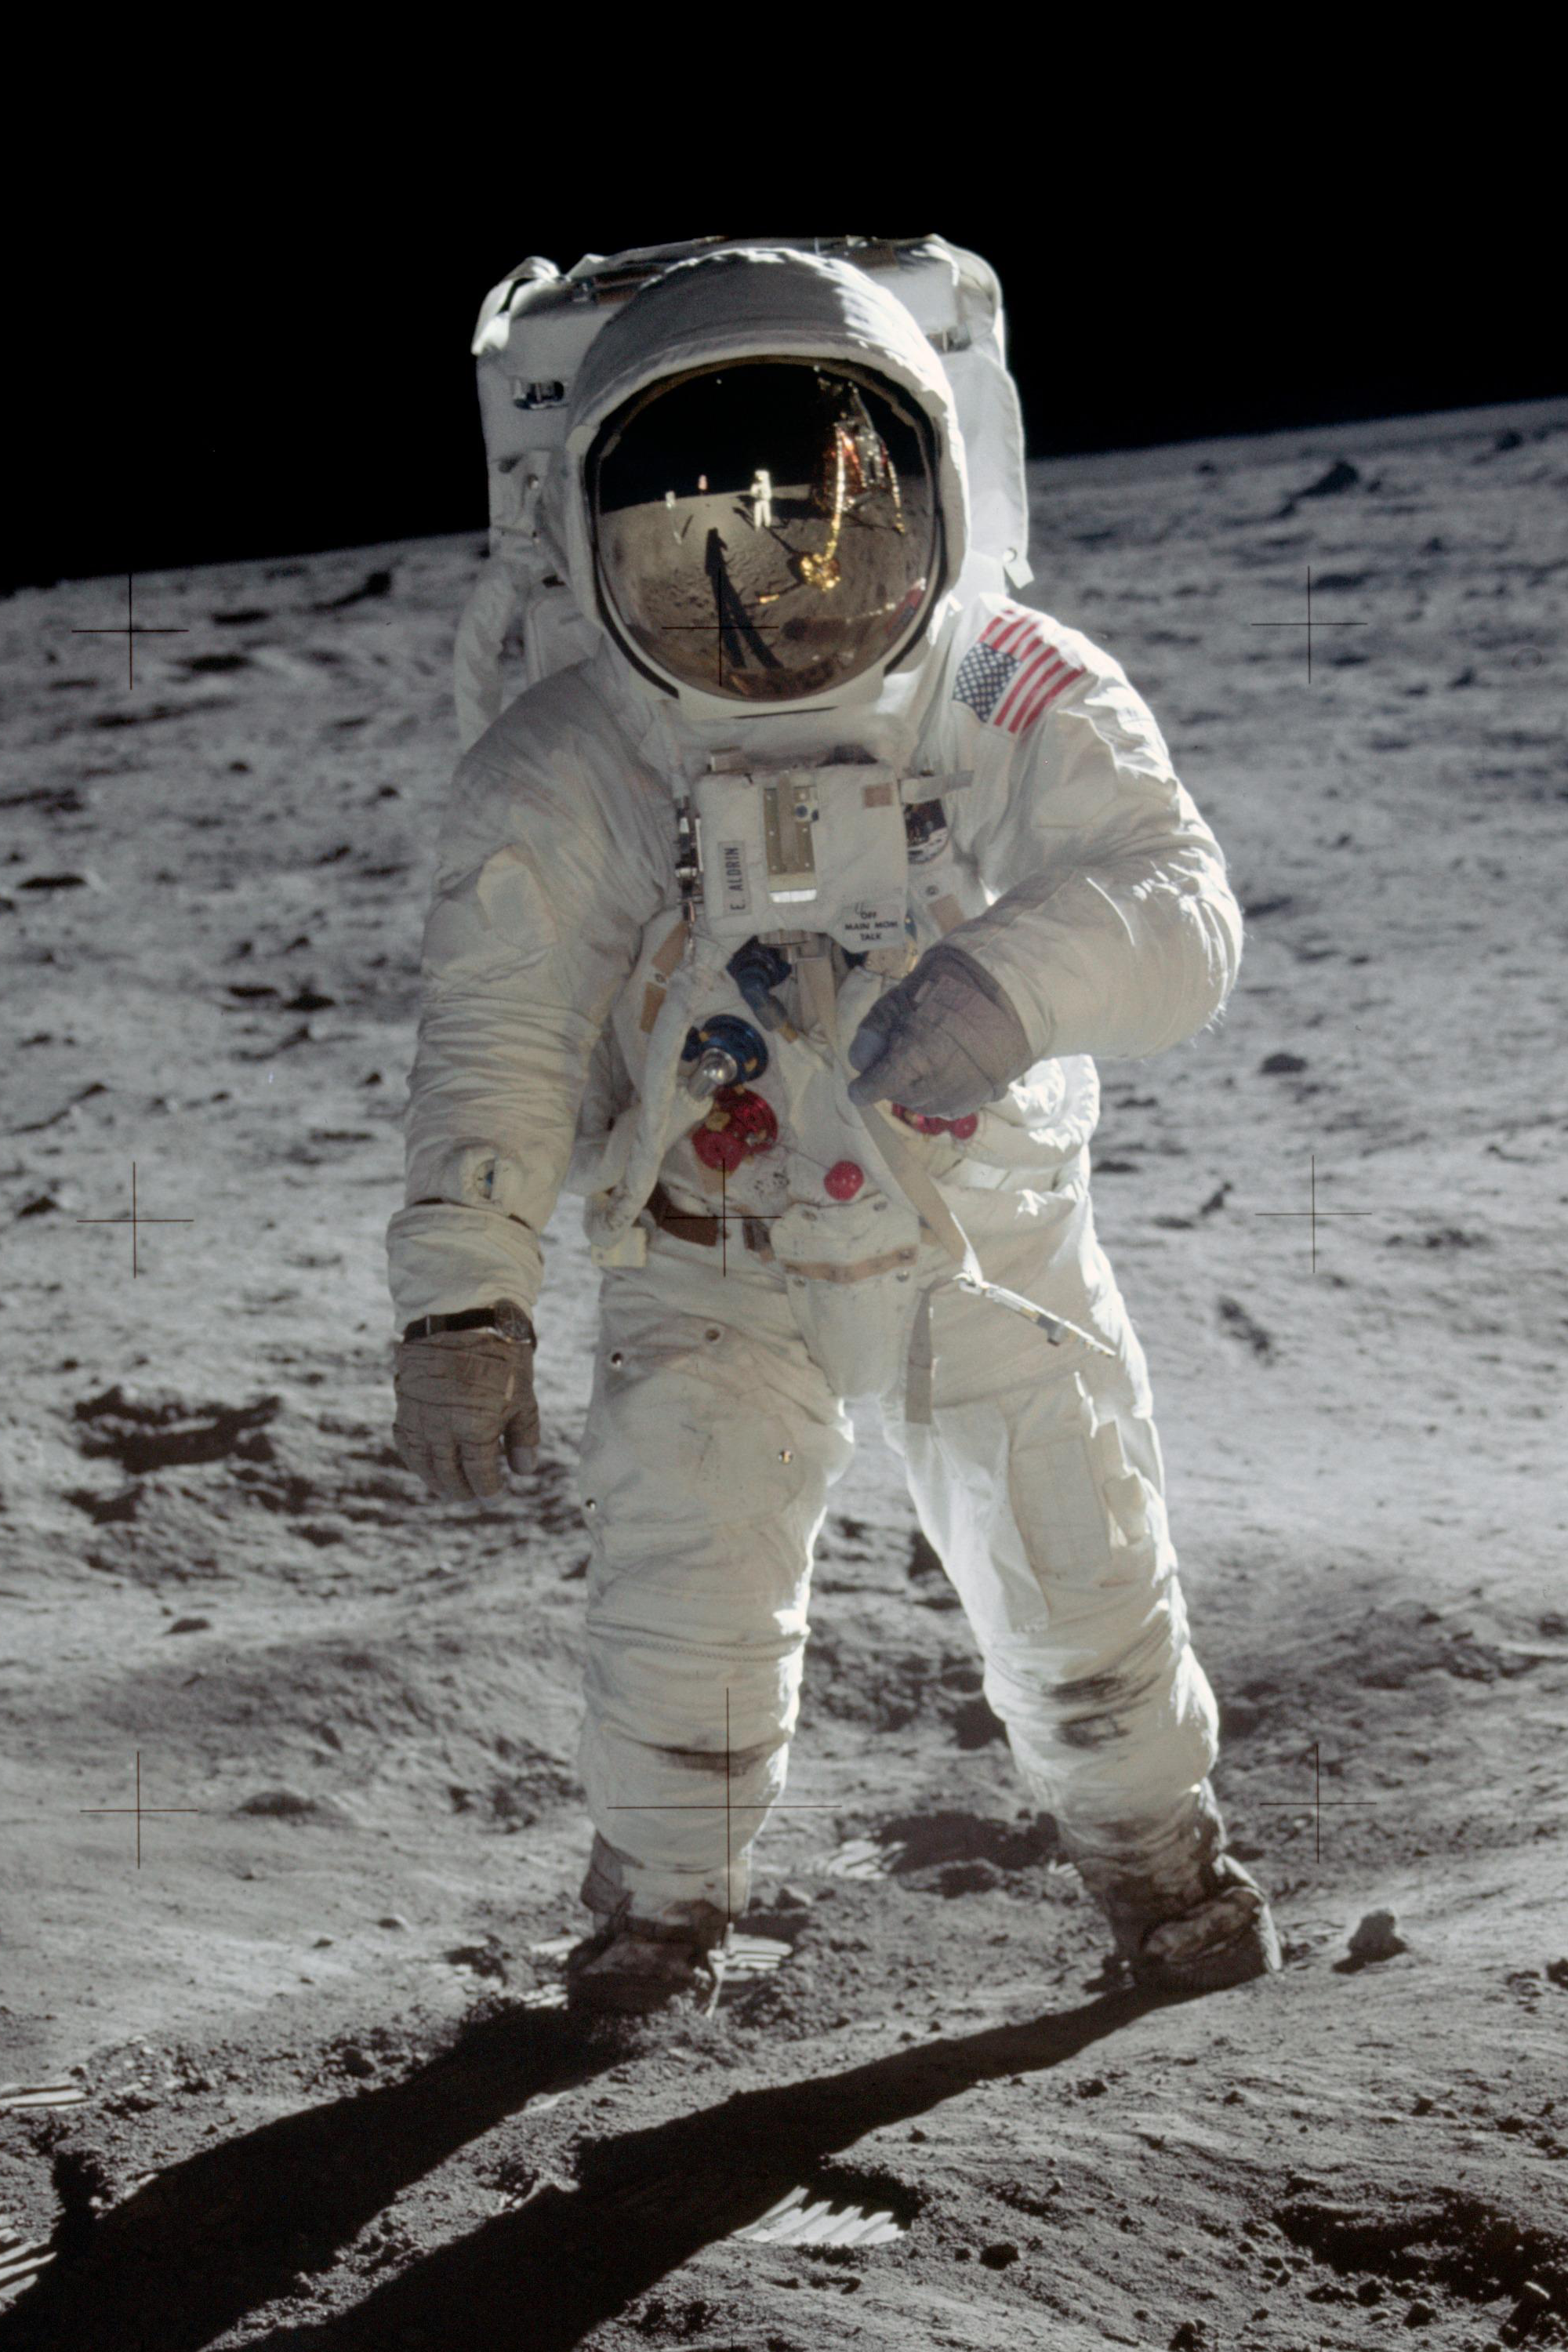
\includegraphics[width = \textwidth]{img/2-theory/aldrin.jpg}
            \caption{obraz wejściowy}
            \label{theory-technics-mask-aldrin-a}
        \end{subfigure}
        \begin{subfigure}{0.49\textwidth}
            \centering
            \includegraphics[width = \textwidth]{img/2-theory/aldrin_mask.png}
            \caption{maska obrazu}
            \label{theory-technics-mask-aldrin-b}
        \end{subfigure}
        \caption{Przykładowy obraz i jego maska.}
        \caption*{\footnotesize{\textbf{Źródło:} {\url{https://www.nasa.gov/sites/default/files/images/337294main_pg62_as11-40-5903_full.jpg}}}}
        \label{theory-technics-mask-aldrin}
        \end{figure}
        
        Aby zastosować maskę należy wykorzystać jej wartości przy sposobie liczenia kary dla danej nitki. Jedną z najprostszych implementacji jest dodanie do wartości otrzymywanej kary średniej wartości pikseli maski znajdującego się na trasie nitki pomnożonego przez pewną stałą. Taką karę wyrazić można za pomocą wzoru:
        
        \begin{equation} \label{theory-technics-mask-penalty}
            P(k, w) = \frac{1}{A} \left[\sum_{i=1}^A k_i + S \cdot \sum_{i=1}^A w_i \right]
        \end{equation}
        gdzie \(k\) to nitka biegnąca przez dwa gwoździe; \(k_i\) to wartość \(i\) piksela przez które przechodzi nitka; \(w\) to wagi nitki biegnącej przez dwa gwoździe; \(w_i\) to wartość wagi \(i\) piksela; \(S\) to współczynnik maski; \(A\) to ilość pikseli przez które przechodzi nitka.
        
        Dzięki zastosowaniu maski oraz odpowiedniego dostosowania algorytmu uzyskane obrazy są bardziej szczegółowe i ostre we wskazanych miejscach, a elementy tła są mniej brane pod uwagę. Należy jednak uważnie dobierać maskę oraz siłę z jaką algorytm ma ją stosować, gdyż może to prowadzić do przesilenia skupiska nitek w~zaznaczonych miejscach i utraty jakichkolwiek detali. Rysunek \ref{theory-technics-mask-aldrin-threaded} przedstawia wyniki algorytmu korzystającego z maski z różnymi wartościami współczynnika maski \(S\) oraz z różną ilością iteracji dla obrazu wejściowego \ref{theory-technics-mask-aldrin-a}. Rysunki od \ref{theory-technics-mask-aldrin-threaded-a} do \ref{theory-technics-mask-aldrin-threaded-e} nie stosują maski i widać, że z każdą kolejną iteracją niemalże równo zapełnia się cały obraz. Tło wtapia się w astronautę i jego obrys jest prawie niewidoczny. Zastosowanie już bardzo niewielkiego współczynnika maski widocznego w obrazach od \ref{theory-technics-mask-aldrin-threaded-f} do \ref{theory-technics-mask-aldrin-threaded-j} skutkuje większym skupieniem na samym astronaucie i jego obrysie. Niestety detale są nadal trudne do odwzorowania, ze względu na dużą szczegółowość obrazu i podobieństwo kolorystyczne powierzchni księżyca i skafandra astronauty. Najbardziej zadowalający wyniki otrzymano na rysunkach \ref{theory-technics-mask-aldrin-threaded-k} oraz \ref{theory-technics-mask-aldrin-threaded-l}, które oprócz użycia relatywnie wysokiego współczynnika zostały wytworzone jedynie przy liczbie iteracji odpowiednio 1500 i 2000. Ostatni rząd rysunków od \ref{theory-technics-mask-aldrin-threaded-p} do \ref{theory-technics-mask-aldrin-threaded-t} pokazuje jak fatalny rezultat otrzymuje się bez zmniejszenia współczynnika maski. Algorytm próbuje odwzorować jedynie kształt astronauty w bardzo agresywny sposób, kompletnie pomijając inne aspekty obrazu.
        
        \begin{figure}[htb] 
        \centering
        \begin{subfigure}{0.19\textwidth}
            \centering
            \includegraphics[width = \textwidth]{img/2-theory/aldrin/000mask-aldrin_ellipse_1500_threaded.png}
            \caption{1500 iteracji, \protect{współczynnik \\ \(S\) = 0.0}}
            \label{theory-technics-mask-aldrin-threaded-a}
        \end{subfigure}
        \begin{subfigure}{0.19\textwidth}
            \centering
            \includegraphics[width = \textwidth]{img/2-theory/aldrin/000mask-aldrin_ellipse_2000_threaded.png}
            \caption{2000 iteracji, \protect{współczynnik \\ \(S\) = 0.0}}
            \label{theory-technics-mask-aldrin-threaded-b}
        \end{subfigure}
        \begin{subfigure}{0.19\textwidth}
            \centering
            \includegraphics[width = \textwidth]{img/2-theory/aldrin/000mask-aldrin_ellipse_2500_threaded.png}
            \caption{2500 iteracji, \protect{współczynnik \\ \(S\) = 0.0}}
            \label{theory-technics-mask-aldrin-threaded-c}
        \end{subfigure}
        \begin{subfigure}{0.19\textwidth}
            \centering
            \includegraphics[width = \textwidth]{img/2-theory/aldrin/000mask-aldrin_ellipse_3000_threaded.png}
            \caption{3000 iteracji, \protect{współczynnik \\ \(S\) = 0.0}}
            \label{theory-technics-mask-aldrin-threaded-d}
        \end{subfigure}
        \begin{subfigure}{0.19\textwidth}
            \centering
            \includegraphics[width = \textwidth]{img/2-theory/aldrin/000mask-aldrin_ellipse_3500_threaded.png}
            \caption{3500 iteracji, \protect{współczynnik \\ \(S\) = 0.0}}
            \label{theory-technics-mask-aldrin-threaded-e}
        \end{subfigure}
        \begin{subfigure}{0.19\textwidth}
            \centering
            \includegraphics[width = \textwidth]{img/2-theory/aldrin/010mask-aldrin_ellipse_1500_threaded.png}
            \caption{1500 iteracji, \protect{współczynnik \\ \(S\) = 0.1}}
            \label{theory-technics-mask-aldrin-threaded-f}
        \end{subfigure}
        \begin{subfigure}{0.19\textwidth}
            \centering
            \includegraphics[width = \textwidth]{img/2-theory/aldrin/010mask-aldrin_ellipse_2000_threaded.png}
            \caption{2000 iteracji, \protect{współczynnik \\ \(S\) = 0.1}}
            \label{theory-technics-mask-aldrin-threaded-g}
        \end{subfigure}
        \begin{subfigure}{0.19\textwidth}
            \centering
            \includegraphics[width = \textwidth]{img/2-theory/aldrin/010mask-aldrin_ellipse_2500_threaded.png}
            \caption{2500 iteracji, \protect{współczynnik \\ \(S\) = 0.1}}
            \label{theory-technics-mask-aldrin-threaded-h}
        \end{subfigure}
        \begin{subfigure}{0.19\textwidth}
            \centering
            \includegraphics[width = \textwidth]{img/2-theory/aldrin/010mask-aldrin_ellipse_3000_threaded.png}
            \caption{3000 iteracji, \protect{współczynnik \\ \(S\) = 0.1}}
            \label{theory-technics-mask-aldrin-threaded-i}
        \end{subfigure}
        \begin{subfigure}{0.19\textwidth}
            \centering
            \includegraphics[width = \textwidth]{img/2-theory/aldrin/010mask-aldrin_ellipse_3500_threaded.png}
            \caption{3500 iteracji, \protect{współczynnik \\ \(S\) = 0.1}}
            \label{theory-technics-mask-aldrin-threaded-j}
        \end{subfigure}
        \begin{subfigure}{0.19\textwidth}
            \centering
            \includegraphics[width = \textwidth]{img/2-theory/aldrin/030mask-aldrin_ellipse_1500_threaded.png}
            \caption{1500 iteracji, \protect{współczynnik \\ \(S\) = 0.3}}
            \label{theory-technics-mask-aldrin-threaded-k}
        \end{subfigure}
        \begin{subfigure}{0.19\textwidth}
            \centering
            \includegraphics[width = \textwidth]{img/2-theory/aldrin/030mask-aldrin_ellipse_2000_threaded.png}
            \caption{2000 iteracji, \protect{współczynnik \\ \(S\) = 0.3}}
            \label{theory-technics-mask-aldrin-threaded-l}
        \end{subfigure}
        \begin{subfigure}{0.20\textwidth}
            \centering
            \includegraphics[width = 0.95\textwidth]{img/2-theory/aldrin/030mask-aldrin_ellipse_2500_threaded.png}
            \caption{2500 iteracji, \protect{współczynnik \\ \(S\) = 0.3}}
            \label{theory-technics-mask-aldrin-threaded-m}
        \end{subfigure}
        \begin{subfigure}{0.19\textwidth}
            \centering
            \includegraphics[width = \textwidth]{img/2-theory/aldrin/030mask-aldrin_ellipse_3000_threaded.png}
            \caption{3000 iteracji, \protect{współczynnik \\ \(S\) = 0.3}}
            \label{theory-technics-mask-aldrin-threaded-n}
        \end{subfigure}
        \begin{subfigure}{0.19\textwidth}
            \centering
            \includegraphics[width = \textwidth]{img/2-theory/aldrin/030mask-aldrin_ellipse_3500_threaded.png}
            \caption{3500 iteracji, \protect{współczynnik \\ \(S\) = 0.3}}
            \label{theory-technics-mask-aldrin-threaded-o}
        \end{subfigure}
        \begin{subfigure}{0.19\textwidth}
            \centering
            \includegraphics[width = \textwidth]{img/2-theory/aldrin/100mask-aldrin_ellipse_1500_threaded.png}
            \caption{1500 iteracji, \protect{współczynnik \\ \(S\) = 1.0}}
            \label{theory-technics-mask-aldrin-threaded-p}
        \end{subfigure}
        \begin{subfigure}{0.19\textwidth}
            \centering
            \includegraphics[width = \textwidth]{img/2-theory/aldrin/100mask-aldrin_ellipse_2000_threaded.png}
            \caption{2000 iteracji, \protect{współczynnik \\ \(S\) = 1.0}}
            \label{theory-technics-mask-aldrin-threaded-q}
        \end{subfigure}
        \begin{subfigure}{0.19\textwidth}
            \centering
            \includegraphics[width = \textwidth]{img/2-theory/aldrin/100mask-aldrin_ellipse_2500_threaded.png}
            \caption{2500 iteracji, \protect{współczynnik \\ \(S\) = 1.0}}
            \label{theory-technics-mask-aldrin-threaded-r}
        \end{subfigure}
        \begin{subfigure}{0.19\textwidth}
            \centering
            \includegraphics[width = \textwidth]{img/2-theory/aldrin/100mask-aldrin_ellipse_3000_threaded.png}
            \caption{3000 iteracji, \protect{współczynnik \\ \(S\) = 1.0}}
            \label{theory-technics-mask-aldrin-threaded-s}
        \end{subfigure}
        \begin{subfigure}{0.19\textwidth}
            \centering
            \includegraphics[width = \textwidth]{img/2-theory/aldrin/100mask-aldrin_ellipse_3500_threaded.png}
            \caption{3500 iteracji, \protect{współczynnik \\ \(S\) = 1.0}}
            \label{theory-technics-mask-aldrin-threaded-t}
        \end{subfigure}
        \caption{Wpływ stosowania maski z różną wartością współczynnika maski w tworzeniu obrazów Thread Art.}
        \label{theory-technics-mask-aldrin-threaded}
        \end{figure}
        
        \subsection{Wizualizacja}  \label{theory-technics-vis}
        Sposób wizualizacji obrazu wyjściowego jest nie mniej ważny od samego procesu tworzenia go. Rozróżnić możemy dwa rodzaje wizualizacji:
        \begin{itemize}
            \item Cyfrowy
            \item Rzeczywisty
        \end{itemize}
        W przypadku tego pierwszego otrzymujemy listę wszystkich nitek wykorzystanych do produkcji obrazu. Jednym z najprostszych sposobów jest wykorzystanie tych wartości, aby na pustym obrazie nanieść linie łączące te punkty. W ten sposób otrzymujemy reprezentację danych z wykorzystaniem grafiki rastrowej.
        
        Inną opcją jest wykorzystanie grafiki wektorowej, której własności idealnie pasują do podanych danych. Aby otrzymać taki obraz należy przy pomocy otrzymanej listy nitek stworzyć obraz składający się z linii, a następnie wyświetlić lub zapisać w postaci pliku SVG. Niewątpliwą zaletą tej formy wizualizacji jest możliwość późniejszego dostosowania rozdzielczości rastrowej reprezentacji zdjęcia, a także wykorzystanie linii lepiej oddających naturę nitek (na przykład linii z antyaliasingiem).
        
        Ostatnią formą wizualizacji danych z algorytmu jest reprezentacja rzeczywista. W tym celu należy fizycznie wykonać ramkę składającą się z określonej wcześniej liczy gwoździ, a następnie postępować zgodnie z otrzymaną z algorytmu listą gwoździ. Finalny efekt zależy od rodzaju użytej nici, a także rozmiaru ramki.
        
        Na rysunku \ref{theory-technics-vis-comp} widnieje ten sam obraz zwizualizowany cyfrowo w postaci mapy bitowej, oraz obraz rzeczywisty, wykonany ręcznie poprzez poprowadzenie nitki przez odpowiednie gwoździe. Dostrzec można, że obie wizualizacje różnią się od siebie pod pewnymi względami. Wizualizacja cyfrowa jest bardziej ostra i wyraźna, natomiast ta rzeczywista wygląda na rozmytą. Niemniej jednak wizualizacja cyfrowa, która jest nieporównywalnie szybsza do utworzenia, jest wystarczającym przybliżeniem wersji rzeczywistej. 
    
        \begin{figure}[htb]
        \centering
        \begin{subfigure}{0.49\textwidth}
            \centering
            \includegraphics[width = \textwidth]{img/2-theory/wiz-cyfrowy.png}
            \caption{wizualizacja cyfrowa}
            \label{theory-technics-vis-comp-a}
        \end{subfigure}
        \begin{subfigure}{0.49\textwidth}
            \centering
            \includegraphics[width = \textwidth]{img/2-theory/wiz-rzeczywisty.png}
            \caption{wizualizacja rzeczywista}
            \label{theory-technics-vis-comp-b}
        \end{subfigure}
        \caption{Przedstawienie wizualizacji cyfrowej i rzeczywistej obrazów Thread Art.}
        \caption*{\footnotesize{\textbf{Źródło:}
        \url{https://www.youtube.com/watch?v=UsbBSttaJos}}}
        \label{theory-technics-vis-comp}
        \end{figure}
            
\chapter{Przegląd istniejących rozwiązań} \label{others}
Technika automatycznego tworzenia obrazów Thread Art liczy już kilka lat, ponieważ zapoczątkowana i opisana została ona w roku 2016. Przez ten czas podejmowane były liczne próby ulepszenia pracy Petrosa. Niektóre z nich były możliwie uproszczoną wersją algorytmu, głównie stworzoną z myślą o wygenerowaniu jednego lub kilku konkretnych dzieł, a inne zawarte były w dokładnie opisanych pracach naukowych zgłębiających techniki i algorytmy tworzenia takich obrazów. W niniejszym rozdziale omówiono cztery wybrane przykładowe implementacje. Opisano całą użytą metodę wraz z zastosowanym algorytmem oraz porównano z metodą standardową opisaną w rozdziale \ref{theory}. Ponadto, przedstawiono wady i zalety opisywanej metody oraz przykładowe obrazy wykonane z jej pomocą.
    \section{Podstawowa metoda autorstwa Jenny Ma} \label{others-jenny}
    Pierwszą, najmniej skomplikowaną metodą generowania obrazów Thread Art, jest metoda przedstawiona przez Jenny Ma. Jest ona inżynierem komputerowym i pasjonatką lotnictwa pochodzącą z Toronto. Celem jej projektu była implementacja od podstaw algorytmu tworzenia obrazów Thread Art oraz finalnie skonstruowanie fizycznej kopii portretu ze ślubu jej rodziców \cite{jenny-youtube}.
        \subsection{Opis rozwiązania}
        Dane wejściowe metody Jenny są bardzo jasno zdefiniowane, stąd ich obróbka była bardzo podstawowa i sprowadzała się jedynie do wczytania zdjęcia jako czarno-białej mapy bitowej oraz przycięcia go do koła o średnicy równej bokowi krótszego boku prostokąta. 
        
        Algorytm Jenny był niezmodyfikowaną podstawową wersją algorytmu opisanego w sekcji \ref{theory-std-method-algorithm}, czyli po wybraniu losowego gwoździa startowego, każdy następny był wybierany na podstawie najmniejszej średniej wartości pikseli, przez które przechodzi dana nitka. 
        
        Dane wyjściowe zostały zwizualizowane zarówno w postaci cyfrowego podglądu, jak i wykonane w rzeczywistości dzięki wygenerowanej przez algorytm liście kolejnych gwoździ do połączenia. Obie wersje przedstawia rysunek \ref{theory-technics-vis-comp}.
        
        Wszystkie parametry zostały dobrane empirycznie tak, aby efekt końcowy wyglądał najlepiej według subiektywnej oceny wizualnej autorki. Użytych zostało trzysta gwoździ, a obraz osiągnął pożądany wygląd po trzech tysiącach iteracji.
        
        Ciekawymi technikami zastosowanymi w wyżej przedstawionej metodzie są sparametryzowanie szerokości nitki w pikselach, które finalnie jednak pozostało w domyślnej wartości równej \mintinline{python}{PIXEL_WIDTH} = 1, oraz dodanie parametru do pominięcia \(n\)~najbliższych gwoździ przy szukaniu najlepszej nitki. Dzięki temu drugiemu algorytm nie skupiał się na wybieraniu jedynie bardzo krótkich nitek, ze względu na ich niską średnią wartość pikseli. Parametr ten ustawiono na wartość \mintinline{python}{NAILS_SKIP} = 10. 

        Rozwiązanie Jenny mimo prostoty było adekwatne do założeń. Wybrany przez nią do odwzorowania portret był odpowiednio przycięty i cechował się niską szczegółowością oraz wysokim kontrastem, dzięki czemu prosty algorytm oparty o średnią wartość pikseli na danej nitce okazał się wystarczający. Stworzeniu filmu opisującego jej rozwiązanie oraz przedstawieniu często nieoczywistych trudności, które napotkała, pozwala na szybkie zrozumienie problemu i uwypuklenie miejsc, które pozwoliłyby usprawnić jej metodę. Ponadto dzięki niskiej liczbie parametrów i prostocie algorytmu jej implementacja działa bardzo szybko, gdyż obrazy testowe o~rozdzielczości zbliżonej do tej opisanej w autorskiej metodzie w rozdziale \ref{mine} były generowane nawet dwukrotnie szybciej.
        
        Niestety metoda ta ma również szereg wad, spośród których największą wydaje się być bardzo niska wszechstronność algorytmu, czyli złe radzenie sobie z obrazami, które nie zostały wybrane z myślą o algorytmie. Wprowadzane do algorytmu dane muszą być danymi bardzo sprzyjającymi (o dużym kontraście, z niską szczegółowością i małą liczbą enklaw segmentacji), aby efekt końcowy był podobny do obrazu wejściowego, a same parametry nie wpływają bezpośrednio na działanie algorytmu. Na rysunku \ref{others-jenny-output} przedstawione zostały obrazy testowe wykonane metodą Jenny. Liczba iteracji każdego obrazu to trzy tysiące, a liczba gwoździ to trzysta. Jak można zauważyć, bardziej skomplikowanym obrazom, takim jak \ref{others-jenny-output-a}, \ref{others-jenny-output-b} i \ref{others-jenny-output-d} brakuje szczegółowości i są zbyt ciemne, natomiast obraz prostszy, taki jak \ref{others-jenny-output-c}, odwzorowany jest poprawnie, lecz posiada sporą ilość szumu, czyli linii, które niewiele poprawiają obraz, a wręcz go pogarszają.
        
        \begin{figure}[htb] 
        \centering
        \begin{subfigure}{0.24\textwidth}
            \centering
            \includegraphics[width = \textwidth]{img/3-others/jenny-out/jenny-aldrin-output.png}
            \caption{Thread Art metodą Jenny Ma prezentujący Buzza Aldrina na Księżycu}
            \label{others-jenny-output-a}
        \end{subfigure}
        \begin{subfigure}{0.24\textwidth}
            \centering
            \includegraphics[width = \textwidth]{img/3-others/jenny-out/jenny-dali-output.png}
            \caption{Thread Art metodą Jenny Ma prezentujący Salvadora Dali}
            \label{others-jenny-output-b}
        \end{subfigure}
        \begin{subfigure}{0.24\textwidth}
            \centering
            \includegraphics[width = \textwidth]{img/3-others/jenny-out/jenny-fawkes-output.png}
            \caption{Thread Art metodą Jenny Ma prezentujący maskę Fawkesa}
            \label{others-jenny-output-c}
        \end{subfigure}
        \begin{subfigure}{0.24\textwidth}
            \centering
            \includegraphics[width = \textwidth]{img/3-others/jenny-out/jenny-taco-output.png}
            \caption{Thread Art metodą Jenny Ma prezentujący Taco Hemingwaya}
            \label{others-jenny-output-d}
        \end{subfigure}
        \caption{Prezentacja obrazów testowych metodą Jenny Ma.}
        \label{others-jenny-output}
        \end{figure}
            
    \section{Metoda wykorzystująca maski autorstwa Calluma McDougalla} \label{others-callum}
    Metoda Colluma jest metodą bardziej skomplikowaną, lecz jej założenia są dość podobne do metody rozwiązania przedstawionego w sekcji \ref{others-jenny}. Metoda ta zamiast skupiać się na jednym obrazie, próbuje dostosować go do szerszego spektrum, lecz nadal podchodzi do każdego z nich indywidualnie poprzez staranny dobór parametrów oraz danych wejściowych \cite{callum-github}.
        \subsection{Opis rozwiązania}
        Metoda Calluma pozwala na generowanie zarówno obrazów kolorowych, obrazów składających się z kilku konkretnych kolorów, ale też obrazów czarno-białych. Na każde z jego dzieł składa się odpowiedni dobór parametrów, wybór algorytmu oraz manualne stworzenie maski. Sprawdza się to tylko w tym jednym konkretnym przypadku oraz wymaga dużych umiejętności przy przygotowaniu danych wejściowych. Opisana tutaj zostanie jedynie metoda najbardziej zbliżonej do tej opracowanej w~rozdziale \ref{mine}, czyli taka, która działa jedynie na obrazach czarno-białych.
        
        Na początku wczytywane są dane wejściowe, czyli obraz wejściowy, który konwertowany jest do tablicy liczbowej. Oprócz tego jednak, w znacznej części ze swoich dzieł Callum korzystał z dodatkowej, stworzonej przez siebie maski, czyli tablicy o~tej samej rozdzielczości co obraz wejściowy, lecz z wartościami z przedziału (0.0;1.0>. Bardziej rozbudowana wersja tej koncepcji, oferująca jednak niewielki wzrost jakości generowanych obrazów, to zastosowanie dwóch masek, z wartościami dodatnimi i ujemnymi. Dzięki temu możliwe było podkreślenie, które fragmenty obrazu powinny być brane pod uwagę przez algorytm bardziej, a które mniej. Na rysunku \ref{others-callum-output-b} zaprezentowana została przykładowa maska.
        
        Sam algorytm, tak jak ma to miejsce w wersji podstawowej, zaczyna od losowego gwoździa i po kolei wybiera następne bazując na najniższej wyliczonej karze. Sposób liczenia kary musiał być jednak dostosowany do przetwarzania zarówno danych pochodzących z maski, jak i samego obrazu. W celu liczenia kary, mając do dyspozycji obraz wejściowy jak i dwie maski (z negatywnymi i pozytywnymi wartościami) kara liczona jest w następujący sposób:
        
        \begin{equation} \label{others-callum-penalty}
            P(k, w) = \frac{1}{N} \left[ \sum_{i=1}^A max(k_i w_i^+, 0) - L \cdot \sum_{i=1}^A min(k_i w_i^-, 0) \right]
        \end{equation}
        gdzie \(k\) to nitka biegnąca przez dwa gwoździe; \(k_i\) to wartość \(i\) piksela przez które przechodzi nitka; \(w^+\) i \(w^-\) to pozytywne i negatywne wagi nitki biegnącej przez dwa gwoździe; \(w_i^+\) i \(w_i^-\) to pozytywne i negatywne wartości wagi \(i\) piksela; \(L\) to współczynnik mówiący z jaką siłą algorytm traktuje ujemne wartości; \(N\) to norma linii, która może być równa ilości pikseli przez które przechodzi nitka, sumie wag, przez które przechodzi nitka lub \(N\) = 1; \(A\) to ilość pikseli przez które przechodzi nitka.
        
        Dane wyjściowe, chodź mogą zostać stworzone ręcznie, zostają zwizualizowane na mapie bitowej. Jasno określonym celem autora było stworzenie obrazów możliwie jak najlepiej wyglądających w podglądzie cyfrowym. 
        
        \newpage
        Na szczególną uwagę w implementacji Calluma zasługuje wykorzystanie słownika pozycji gwoździ i nitek. Jest to proces, który zajmuje zdecydowanie najwięcej czasu, a dzięki wygenerowaniu tych wartości wcześniej użytkownik jest w stanie eksperymentować z wartościami parametrów i masek tak, aby osiągnąć jak najlepszy wynik, nie musząc przy tym każdorazowo czekać kilka, lub nawet kilkanaście minut. 
        
        Ze względu dla charakter metody Calluma, zamiast obrazów testowych, na rysunku \ref{others-callum-output} widać obraz jego autorstwa(\ref{others-callum-output-c}), do którego parametry zostały indywidualnie dobrane, obraz wejściowy(\ref{others-callum-output-a}) oraz maskę(\ref{others-callum-output-b}) specjalnie stworzoną do tego problemu. 
        
        \begin{figure}[htb] 
        \centering
        \begin{subfigure}{0.32\textwidth}
            \centering
            \includegraphics[width = \textwidth]{img/3-others/callum-churchill-monochrome.jpg}
            \caption{obraz Winstona Churchilla}
            \label{others-callum-output-a}
        \end{subfigure}
        \begin{subfigure}{0.32\textwidth}
            \centering
            \includegraphics[width = \textwidth]{img/3-others/callum-churchill-weighting.jpg}
            \caption{maska obrazu wejściowego}
            \label{others-callum-output-b}
        \end{subfigure}
        \begin{subfigure}{0.32\textwidth}
            \centering
            \includegraphics[width = \textwidth]{img/3-others/callum-churchill-output.jpg}
            \caption{wygenerowany obraz, 3500 iteracji, 180 gwoździ}
            \label{others-callum-output-c}
        \end{subfigure}
        \caption{Prezentacja obrazu autorstwa Calluma McDougalla.}
        \label{others-callum-output}
        \end{figure}
        
    \section{Metoda Birsaka, Rista, Wonki i Musialskiego} \label{others-birsak}
    Metoda zaprezentowana w pracy ``String Art: Towards Computational Fabrication of String Images'' \cite{article-string-art-birsak} przedstawia podejście inne niż pozostałe opisane wcześniej. Największy nacisk kładziony jest tam na możliwe najdokładniejsze automatyczne odwzorowanie obrazu w formie rzeczywistej oraz zastosowanie algorytmu biorącego całość obrazu pod uwagę przy wyborze ścieżki nici. 
    
        \subsection{Opis rozwiązania}
        Autorzy pracy przedstawili na początku spis założeń dotyczących projektu, które muszą spełnić, aby możliwie jak najdokładniej spełnić oryginalne założenia autora techniki. Są to:
        \begin{itemize}
            \item (R1): Fizyczna nitka jest całkowicie nieprzezroczysta, przez co wielokrotne rysowanie tego samego sznurka daje ten sam wynik;
            \item (R2): Stosunek rozmiaru płótna do grubości nitki jest stały, dzięki czemu model jest niezależny od użytej grubości sznurka oraz rozmiaru ramki;
            \item (R3): Uwzględniana zostaje średnica gwoździa, co oznacza, że połączenie między dwoma pinami w praktyce może być narysowane na cztery różne sposoby, jak pokazano na rysunku \ref{birsak-edges};
            \item (R4): Dane wyjściowe algorytmu muszą być możliwe do fabrykacji przy użyciu jednej długiej nici, co oznacza, że ostatecznie wygenerowana ścieżka musi być ścieżką eulerowską
        \end{itemize}
        
        \begin{figure}[htb]
            \centering
            \includegraphics[width=\textwidth,keepaspectratio]{img/3-others/birsak-edges.png}
            \caption{Wizualizacja możliwych połączeń miedzy dwoma gwoździami w metodzie Birsaka, Rista, Wonki i Musialskiego.}
            \caption*{\footnotesize{\textbf{Źródło:} {\url{https://www.researchgate.net/publication/322766118_String_Art_Towards_Computational_Fabrication_of_String_Images}}}}
            \label{birsak-edges}
        \end{figure}
    
        Obrazami wejściowymi są czarno-białe obrazy o proporcjach 1:1. Są to głównie portrety, lecz ze względu na wszechstronność algorytmu wśród demonstracyjnych obrazów znajdują się także symbole, rysunki oraz zdjęcia zwierząt. Sam obraz reprezentowany jest w postaci macierzy, gdzie wiersze odpowiadają kolejnym pikselom, a kolumny wartościom przez które przechodzi nitka. Ponadto, zdecydowano się na zastosowanie dodatkowej maski z wagami, która później wykorzystana jest przy liczeniu dopasowania poszczególnych nitek.
        
        Algorytm zaproponowany w pracy traktuje problem bardziej globalnie. Nie zaczyna on od wybrania losowego gwoździa, a następnie wyznaczenia trasy nitki pojedynczo. Zamiast tego na początku liczone są wartości dopasowania wszystkich możliwych nitek, które poprowadzić można przez gwoździe. Następnie wybierane są każdorazowo najlepsze możliwe nitki tak, aby powstała z nich ścieżka była ścieżką eulerowską. Algorytm dodaje kolejne nitki tak długo, jak dodanie jej do obrazu spowoduje polepszenie jego jakości, lub przez określoną przez użytkownika liczbę razy.
        
        Sam algorytm liczenia dopasowania jest zupełnie inny niż ten opisany w sekcji \ref{theory-std-method-algorithm}. Wykorzystuje binarną nieliniową metodę najmniejszych kwadratów oraz liczony jest w następujący sposób:
        
        \begin{equation} \label{others-birsak-penalty}
            \min_x ||WF(x) - Wy||_2^2
        \end{equation}
        gdzie \(x\) to obraz wejściowy; \(F(x)\) to autorskie mapowanie krawędzi do pikseli; \(W\) to wagi pikseli; \(y\) to obraz wyjściowy.
        
        Oprócz cyfrowej wizualizacji wygenerowanych obrazów twórcy postanowili zaprogramować ramię robota tak, aby ten w automatyczny sposób był w stanie stworzyć rzeczywistą reprezentację obrazu. Jest to jednak funkcja, która nie dotyczy tematu niniejszej pracy magisterskiej, więc jej opis zostanie pominięty. 

        Powyżej opisana metoda skupiona jest wokół tworzenia rzeczywistych dzieł i~według opisanych w pracy wyników przewyższa skutecznością inne implementacje, zarówno biorąc pod uwagę ocenę subiektywną, jak i matematyczną, wykorzystującą wartość pierwiastka z odchylenia średniokwadratowego. Dodatkowo, dzięki zastosowaniu maski z wagami, algorytm lepiej odwzorowuje szczegóły obrazu, kosztem mniej istotnych elementów, wymagając przy tym jednak bardziej skomplikowanego przygotowania danych wejściowych.
        
        Na rysunku \ref{others-birsak-output} przedstawiono po kolei obraz wejściowy, cyfrową wizualizację działania algorytmu autorów, jego rzeczywistą wizualizację oraz oryginalną pracę Petrosa Vrellisa. Obraz autorów porównywany przy pomocy wartości pierwiastka z~odchylenia średniokwadratowego osiągnął wynik bardziej zbliżony do oryginału, niż obraz Petrosa. W ocenie subiektywnej jednak ten sam obraz zawiera mniej szczegółów i jest bardziej rozmazany. Warto natomiast dodać, że obraz Petrosa zawiera więcej szumów związanych z generowaniem linii na białej twarzy postaci, co ma miejsce w mniejszym stopniu w pracy autorów.
        \begin{figure}[htb]
            \centering
            \includegraphics[width=\textwidth,keepaspectratio]{img/3-others/birsak-vs-petros.png}
            \caption{Zestawienie wyników pracy Birsaka, Rista, Wonki i Musialskiego z obrazem Petrosa Vrellisa.}
            \caption*{\footnotesize{\textbf{Źródło:} {\url{https://www.researchgate.net/publication/322766118_String_Art_Towards_Computational_Fabrication_of_String_Images}}}}
            \label{others-birsak-output}
        \end{figure}

    \section{Metoda Xiaonana Fanga, Bina Liu oraz Ariela Shamira} \label{others-xiao}
    Ostatnią opisywaną tu metodą jest pierwsza praca naukowa powstała zaraz po opublikowaniu przez Petrosa jego artykułu, czyli ``Automatic thread painting generation'' autorstwa Xiaonana Fanga, Bina Liu oraz Ariela Shamira. W odróżnieniu od wcześniej omawianej metody autorzy skupili się jedynie na algorytmie i reprezentacji cyfrowej obrazów, a także przeprowadzili eksperymenty sprawdzające skuteczność swojego algorytmu przy porzuceniu pewnych założeń, takich jak na przykład zasada ciągłości, czyli możliwość utworzenia obrazu z jednej, nieprzerwanej nici.
    
        \subsection{Opis rozwiązania}
        Pierwszą wyróżniającą się rzeczą w tej metodzie jest zastosowanie innej formy reprezentacji nitek na obrazie. Zamiast standardowej formy dwóch punktów (określających początek i koniec nitki), autorzy oznaczyli zbiór wszystkich cięciw na okręgu za pomocą jedynie dwóch parametrów, gdzie każdy oznacza kąt biegunowy dwóch punktów końcowych.
        
        Problem znalezienia uporządkowanej listy nitek spełniających wymagania portretu typu Thread Art potraktowany został tu globalnie. Liczona w tym celu jest wartość dopasowania każdej z nitek, a następnie wybierana jest ich określona liczba z największą wartością, pamiętając jednak o zachowaniu ciągłości nitki w obrazie. Autorzy umożliwili również pracę algorytmu do momentu, aż dodana do obrazu końcowego nitka pogorszy jego jakość, zamiast poprawiać, a także przedstawili wzór na określenie przybliżonej potrzebnej liczby iteracji algorytmu bazując na średniej wartości piksela obrazu wejściowego. Dokładniej opisane zostało to w sekcji \ref{theory-technics-auto-param}
        
        Ze względu na przygotowanie algorytmu do pracy na możliwie jak najszerszej liczbie obrazów, autorzy postanowili zaimplementować algorytm zwiększania kontrastu oraz prostej maski z wagami równymi odpowiednio \(W\) = 2.0 dla ważnych regionów obrazu oraz \(W\) = 1.0 dla pozostałych.
        
        Ponieważ krótkie nitki obejmują mniejszą liczbę pikseli, są tym samym podatne na fałszywie wysoką wartość dopasowania, co skutkuje nadmiernym rysowaniem na marginalnym obszarze koła. W odróżnieniu od rozwiązania autorstwa Jenny Ma opisanego w sekcji \ref{others-jenny}, autorzy tej metody zastosowali parametr premiujący linie dłuższe tak, aby ten niepożądany efekt nie występował tak często. 
        
        Obrazy w ten sposób wygenerowane są następnie wyświetlane w formie cyfrowej. Twórcy zestawili swoje obrazy z obrazami wygenerowanymi w sposób iteratywny (tworząc drogę od pierwszego do ostatniego gwoździa po kolei) oraz eksperymentalnie, obrazami wygenerowanymi ich metodą lecz bez stosowania zasady ciągłości (koniec jednej nitki nie musi być początkiem kolejnej). Wyniki przedstawione są na rysunku \ref{przyklad-testowy-xin}. Zauważyć można, że metoda zaprezentowana w pracy oferuje znacznie lepsze rezultaty, głównie na krawędziach obrazu, w porównaniu do metody iteracyjnej. Co ciekawe, porzucenie zasady ciągłości nie ma dużego wpływu na jakość generowanych obrazów, głównie za sprawą optymalnego dobierania ścieżki nitki w~algorytmie oraz zastosowaniu techniki cofnięcia wyboru danej nitki, gdy wybór jej skutkuje brakiem następnych korzystnych nitek. 
        \begin{figure}[htb]
            \centering
            \includegraphics[width=\textwidth,keepaspectratio]{img/3-others/xin-vs-greedy.png}
            \caption[Zestawienie wyników pracy Xiaonana Fanga, Bina Liu oraz Ariela Shamira z obrazami generowanymi iteratywnie.]{Zestawienie wyników pracy Xiaonana Fanga, Bina Liu oraz Ariela Shamira z obrazami generowanymi iteratywnie. \\ a) oryginał; b) metoda iteracyjna; c) metoda autorska; d) metoda autorska bez zasady ciągłości nitki.}
            \caption*{\footnotesize{\textbf{Źródło:} {\url{https://arxiv.org/abs/1802.04706}}}}
            \label{przyklad-testowy-xin}
        \end{figure}
            
        
\chapter{Autorska metoda generowania obrazów} \label{mine}
Opisywany problem niesie za sobą wiele fizycznych ograniczeń, dokładniej opisanych w rozdziale \ref{theory-std-method}. Nawet używając dobrze przystosowanych danych, wyniki algorytmu mogą być niezadowalające. Z pomocą przychodzą wtedy takie techniki jak używanie masek z wagami czy korekta kolorów obrazu wejściowego. Należy jednak w tym celu posiadać podstawową wiedzę na temat obróbki i tworzenia grafiki komputerowej oraz żmudnie eksperymentować w celu osiągnięcia nieco lepszego wyniku. Istnieje jednak szereg algorytmów mogących w zupełnie automatyczny sposób poprawić jakość generowanych obrazów pozostawiając użytkownikowi jedynie kilka zmiennych aktywnie wpływających na właściwości efektu końcowego. 

Wiele istniejących metod wytwarzania obrazu korzysta z najprostszej wersji algorytmu i nie oferuje możliwości dostosowywania parametrów pracy algorytmu, a~jedynie ilości wykorzystanych gwoździ lub rozdzielczości. Pozostała część rozwiązań wymaga od użytkownika dogłębnego zrozumienia algorytmu w celu doboru parametrów oraz starannego przygotowania danych wejściowych, a co za tym idzie umiejętności obróbki grafiki i programowania. Utrudnia, a wręcz uniemożliwia to użytkownikom stworzenie własnego obrazu w stylu Thread Art. Metoda opisana poniżej rozwiązuje ten problem wykorzystując sztuczną inteligencję oraz podstawowe operacje manipulacji obrazu w celu automatycznego ulepszenia danych wejściowych i efektywnego zwiększenia jakości generowanych obrazów Thread Art. Za sprawą kilku jasno opisanych parametrów użytkownik jest w stanie manipulować doborem nitek tak, aby podkreślić ważne dla obrazu cechy i osiągnąć pożądany efekt, możliwie jak najbardziej przypominający obraz wejściowy. Niniejsza metoda została stworzona głównie z myślą o tworzeniu wizualizacji cyfrowych portretów typu Thread Art, lecz dzięki wygenerowaniu uporządkowanej liście kolejnych gwoździ, istnieje także możliwość stworzenia jego reprezentacji rzeczywistej. 

    \section{Dane wejściowe} \label{mine-input}
    Praca algorytmu zaczyna się od wczytania dowolnego obrazu typu JPEG lub PNG oraz przekonwertowania go do obrazu w odcieniach szarości, czyli takiego o jednym 8-bitowym kanale. Obraz ten zostaje dalej zapisany w postaci dwuwymiarowej macierzy i służy do późniejszego liczenia dopasowania nitek.
    
    Następnym krokiem jest automatyczne przygotowanie maski z wagami dla obrazu wejściowego. Ze względu na to, że takim obrazem może być dowolne zdjęcie lub rysunek, koniecznym jest posłużenie się sztuczną inteligencją, która zadecyduje jakie elementy obrazu są istotne, a który nie. W tym celu używany jest pretrenowany model sieci neuronowej usuwania tła z obrazu \cite{rembg}. Założono tutaj, że w większości obrazów tło jest mniej istotne niż obiekt pierwszoplanowy. W rezultacie otrzymujemy obraz identyczny jak wejściowy, jednak piksele które wykryte zostały jako tło są oznaczone jako przeźroczyste. Obraz ten posłuży dalej do tworzenia maski.
    
    Następnym krokiem jest automatyczne wykrycie krawędzi obrazu wejściowego. W obrazach Thread Art wiele szczegółów zostaje utraconych, ze względu na konieczność używania jedynie cięciw okręgu, muszących przecinać zarówno porządne jak i nieporządne obszary. Stworzenie maski, która promuje kontury obrazu, potrafi znacznie uwypuklić linie tworzące obrys obiektu i jego szczegóły, dzięki czemu wygenerowany obraz znacznie bardziej przypomina ten wejściowy. W celu wygenerowania krawędzi obrazu zastosowano operator Sobla. Polega to na operacji splotu wykonanej na obrazie wejściowym przy pomocy macierzy będącej filtrem (jądrem). Jądro to macierz 3 x 3 składająca się z różnie ważonych indeksów. Obraz jest najpierw przetwarzany osobno pionowo i poziomo, a następnie łączony razem, tworząc nowy obraz, który reprezentuje sumę krawędzi. Na koniec wartości maski są skalowane do sparametryzowanego przedziału <0;\mintinline{python}{MASK_EDGES_FOCUS}>. Wygenerowany w ten sposób obraz jest użyty do utworzenia maski.
    
    Ostatnim etapem jest stworzenie finalnej maski. Na początku tworzona jest macierz o wymiarach takich jak przeskalowany obraz wejściowy. Wartość każdego piksela to suma wartości wszystkich parametrów maski, czyli \mintinline{python}{MASK_BACKGROUND_FOCUS}, \mintinline{python}{MASK_OBJECT_FOCUS} oraz \mintinline{python}{MASK_EDGES_FOCUS}. Następnie każdy piksel, który wykryty został jako tło, jest zmniejszany o stałą wartość tła maski, która jest określona w parametrze \mintinline{python}{MASK_BACKGROUND_FOCUS}. Jeśli natomiast dany piksel nie jest tłem, jego wartość zostaje pomniejszona o wartość skupienia obiektu maski (\mintinline{python}{MASK_OBJECT_FOCUS}) oraz wartości wykrytych krawędzi (\mintinline{python}{mask[i, j]}). Dobór wyżej wymienionych wartości jest kluczowy do działania algorytmu, gdyż określa proporcję poszczególnych elementów maski, a tym samym znacząco wpływa na działanie algorytmu. Dokładny opis wszystkich parametrów metody, a także przykłady jak ich wartości wpływają na wygenerowaną maskę oraz efekt końcowy znajdują się w sekcji \ref{mine-param}. 
    
    Po stworzeniu maski bazowy obraz wejściowy jest poddawany korekcji kontrastu, opisanej dokładniej w rozdziale \ref{theory-std-method-input}.
    
    Rysunki \ref{mine-input-1} oraz \ref{mine-input-2} przedstawiają wszystkie wyżej wymienione techniki na przykładowym obrazie.
    \begin{figure}[htb] 
        \centering
        \begin{subfigure}{0.49\textwidth}
            \centering
            \includegraphics[width = \textwidth]{img/4-mine/input-input.png}
            \caption{obraz wejściowy bez żadnych modyfikacji}
            \label{mine-input-1-a}
        \end{subfigure}
        \begin{subfigure}{0.49\textwidth}
            \centering
            \includegraphics[width = \textwidth]{img/4-mine/input-input_c20.png}
            \caption{obraz wejściowy ze zwiększonym kontrastem}
            \label{mine-input-1-b}
        \end{subfigure}
        \caption{Wizualizacja obrazu wejściowego i zmiany kontrastu autorskiej metody.}
        \label{mine-input-1}
    \end{figure}
        
    \begin{figure}[htb] 
        \centering        
        \begin{subfigure}{0.32\textwidth}
            \centering
            \includegraphics[width = \textwidth]{img/4-mine/input-image_no_bg_alpha.png}
            \caption{obraz wejściowy bez tła\\\hphantom{ }}
            \label{mine-input-2-a}
        \end{subfigure}
        \begin{subfigure}{0.32\textwidth}
            \centering
            \includegraphics[width = \textwidth]{img/4-mine/input-image_edges.png}
            \caption{krawędzie obrazu wejściowego}
            \label{mine-input-2-b}
        \end{subfigure}
        \begin{subfigure}{0.32\textwidth}
            \centering
            \includegraphics[width = \textwidth]{img/4-mine/input-mask.png}
            \caption{finalna maska obrazu wejściowego}
            \label{mine-input-2-c}
        \end{subfigure}
        \caption{Wizualizacja obrazu bez tła, wykrytych krawędzi i finalnej maski dla autorskiej metody.}
        \label{mine-input-2}
        \end{figure}
    
    \section{Generowanie słowników pozycji} \label{mine-dict}
    Jedną z najbardziej wymagających obliczeniowo operacji koniecznych do wygenerowania obrazu Thread Art jest obliczenie pozycji gwoździ na obrazie oraz wszystkich dozwolonych linii łączących te punkty. Aby uniknąć konieczności generowania tych wartości każdorazowo podczas tworzenia obrazu stworzono osobny program służący temu celowi oraz zapisujący wartości w postaci słownika do pliku binarnego. Taka metoda pozwala na natychmiastowy dostęp do danych wszystkich nitek biegnących od danego gwoździa, czy wszystkich punktów leżących między dwoma gwoździami, bez konieczności każdorazowego wykonywania długotrwałych obliczeń. Ponadto, zdefiniowane zostało kilka rodzajów rozmieszczenia gwoździ na płótnie, dzięki czemu możliwe jest tworzenie obrazów z gwoździami rozmieszczonymi na obwodzie prostokąta o proporcjach 2:3, 3:2, 3:4, 4:3 i 1:1 oraz na elipsach wpisanych w te prostokąty. 
    
    Operacja rozpoczyna się od zdefiniowania najpopularniejszych proporcji wśród obrazów \cite{aspect-ratio-youtube}, do których przycinane będą wczytywane obrazy. Przycinane są one zawsze do najbliższych zdefiniowanych proporcji. Następnie zdefiniowano rozdzielczości, do których będą one skalowane, są to: 1561x1561 (1:1), 1761x1321 (4x3) oraz 1801x1441 (5x4). Liczba pikseli w każdym obrazie jest zbliżone, dzięki czemu czas generowania obrazu jest podobny, niezależnie od jego wejściowych proporcji. W przypadku odwrócenia proporcji wykorzystywane są te same wartości, natomiast obraz w czasie tworzenia jest obrócony o $90^\circ$. Następnym krokiem jest wygenerowanie pozycji gwoździ. Algorytm rozmieszcza je równomiernie na obwodzie elipsy lub prostokąta, a ich liczba jest wyliczana na podstawie podanej odległości miedzy nimi, czyli parametru \mintinline{python}{NAIL_DISTANCE}.
    
    Rezultatem są dwie listy i dwa słowniki. Listy przechowują wartości współrzędnych wszystkich gwoździ oraz wszystkie dopuszczalne pary współrzędnych tworzących nitki. Słowniki mapują konkretny gwóźdź do wszystkich wychodzących z niego nitek oraz konkretną nitkę do wszystkich pikseli, przez które przechodzi. 
    
   Po wygenerowaniu, wartości są zapisywane do pliku binarnego, skąd mogą być w~dowolnej chwili wczytane i posłużyć do szybkiego wygenerowania obrazu przez algorytm. Na rysunku \ref{wlasne-dane-slownikowe} zaprezentowane zostały przykładowe użycia słownika w~celu otrzymania danych z obrazu o rozdzielczości 121x161 oraz o odległości miedzy gwoździami \mintinline{python}{NAIL_DISTANCE} = 20.
    \begin{figure}[htb] 
    \centering
    \begin{subfigure}{0.49\textwidth}
        \centering
        \includegraphics[width = \textwidth]{img/4-mine/nails-on-elipse.png}
        \caption{wszystkie gwoździe rozmieszczone w równych odstępach na elipsie}
        \label{wlasne-dane-slownikowe-1}
    \end{subfigure}
    \begin{subfigure}{0.49\textwidth}
        \centering
        \includegraphics[width = \textwidth]{img/4-mine/nails-on-rectangle.png}
        \caption{wszystkie gwoździe rozmieszczone w równych odstępach na prostokącie}
        \label{wlasne-dane-slownikowe-2}
    \end{subfigure}
    \begin{subfigure}{0.49\textwidth}
        \centering
        \includegraphics[width = \textwidth]{img/4-mine/threads-from-nail-of-elipse.png}
        \caption{wszystkie nitki wychodzące z jednego gwoździa na elipsie}
        \label{wlasne-dane-slownikowe-3}
    \end{subfigure}
    \begin{subfigure}{0.49\textwidth}
        \centering
        \includegraphics[width = \textwidth]{img/4-mine/threads-from-nail-of-rectangle.png}
        \caption{wszystkie nitki wychodzące z jednego gwoździa na prostokącie}
        \label{wlasne-dane-slownikowe-4}
    \end{subfigure}
    \begin{subfigure}{0.49\textwidth}
        \centering
        \includegraphics[width = \textwidth]{img/4-mine/points-from-thread-of-elipse.png}
        \caption{wszystkie piksele wychodzące z jednej nitki na elipsie}
        \label{wlasne-dane-slownikowe-5}
    \end{subfigure}
    \begin{subfigure}{0.49\textwidth}
        \centering
        \includegraphics[width = \textwidth]{img/4-mine/points-from-thread-of-rectangle.png}
        \caption{wszystkie piksele wychodzące z jednej nitki na prostokącie}
        \label{wlasne-dane-slownikowe-6}
    \end{subfigure}
    \caption{Wizualizacja danych wejściowych autorskiej metody.}
    \label{wlasne-dane-slownikowe}
    \end{figure}
    
    \section{Opis algorytmu} \label{mine-algorithm}
    Mając wszystkie niezbędne dane wejściowe program zaczyna liczyć najlepszą możliwą trasę dla nitki. Zastosowany został tu algorytm iteracyjny, gdzie wybierany jest pierwszy losowy gwóźdź, a każdy następny jest określany przez funkcję dopasowującą. Ze względu na użycie maski z wagami, do policzenia dopasowania (w formie kary) użyta została średnia ważona. Dla każdego piksela jest ona liczona następująco: 
    
    \begin{equation} \label{mine-algorithm-penalty}
        P(k, w) = \frac{1}{V} \sum_{i=1}^A w_i k_i
    \end{equation}
    gdzie \(k\) to nitka biegnąca przez dwa gwoździe; \(k_i\) to wartość \(i\) piksela przez które przechodzi nitka; \(w\) to wagi nitki biegnącej przez dwa gwoździe; \(w_i\) to wartości wagi \(i\) piksela; \(A\) to ilość pikseli przez które przechodzi nitka; \(V\) to suma wag pikseli, przez które przechodzi nitka.
    
    Algorytm liczy wartość kary na podstawie pikseli obrazu wejściowego i wartości wag wygenerowanej maski. W odróżnieniu od innych metod, nie jest tu parametryzowana jedynie siła, z jaką maska powinna zostać zastosowana, ale jak silnie każdy z jej elementów składowych powinien być brany pod uwagę. Dokładny opis parametrów i to w jaki sposób wpływają one na obraz zostało dokładniej opisane w sekcji \ref{mine-param}.
    
    Ponadto, podobnie jak ma to miejsce w pracy autorstwa Xiaonana Fanga, Bina Liu oraz Ariela Shamira \cite{article-string-art-xiaonan}, autorska metoda oferuje kilka możliwości wyboru momentu zapisania obrazu. Tryb iteracyjny określa minimalną i maksymalną liczbę iteracji oraz interwał z jakim zapis ma zostać dokonany. Tryb automatyczny liczy preferowaną liczbę iteracji na podstawie średniej wartości piksela obrazu wejściowego i zapisuje obraz w tej wyliczonej wartości oraz w wartości powiększonej i pomniejszonej o parametr \mintinline{python}{SAVE_AROUND}. Dokładna liczba preferowanych iteracji liczona jest ze wzoru:
    \begin{equation} \label{mine-algorithm-iterations}
        I(x) = 500 + D \cdot 10 \cdot (255 - M(x)) \cdot S
    \end{equation}
    gdzie \(M(x)\) to średnia wartość pikseli obrazu wejściowego; \(D\) określa parametr \mintinline{python}{PREFERRED_DARKNESS}; \(S\) to parametr ułożenia gwoździ równy \(S\) = 1.0 w przypadku elipsy oraz \(S = \frac{4}{\pi}\) w przypadku prostokąta.
    
    \section{Parametry} \label{mine-param}
    W celu dostosowania algorytmu pod konkretny rodzaj obrazu, ale także subiektywnych preferencji, program oferuje szereg parametrów, których zmiana ma istotny wpływ na wynik końcowy.
    
    Mimo, że parametry programu do generowania pozycji gwoździ i nitek zostały precyzyjnie dobrane, użytkownik nadal posiada możliwość ich modyfikacji. Poniżej znajduje się ich lista oraz dokładny opis:
    \begin{itemize}
        \item \mintinline{python}{NAIL_DISTANCE} określa w jakich odstępach od siebie generowane są gwoździe.
        \item \mintinline{python}{SKIP_NEIGHBOUR_NAILS} określa ile najbliższych gwoździ powinno być ignorowanych przy tworzeniu listy wszystkich możliwych nitek. Parametr ten dotyczy tylko ułożenia gwoździ na elipsie, gdyż w przypadku prostokąta automatycznie usuwane są nitki całkowicie znajdujące się na krawędzi prostokąta.
        \item Rozdzielczości i proporcje określone i opisane w sekcji \ref{mine-dict} również mogą zostać zmienione. Pamiętać należy jednak o tym, aby po zmianie tych parametrów wygenerować na nowo słowniki oraz dostosować algorytm do wczytania nowych danych.
    \end{itemize}
    
    Najważniejszymi parametrami są parametry algorytmu tworzącego obraz. Poniżej znajdują się parametry wraz z opisami dotyczącymi odpowiednio obróbki danych wejściowych, współczynników maski bezpośrednio sterujących algorytmem oraz samego algorytmu:
    \begin{itemize}
        \item \mintinline{python}{CONTRAST_FACTOR} to parametr mówiący z jaką siłą należy zwiększyć kontrast obrazu wejściowego. Każda wartość niższa niż 1.0 zmniejszy kontrast obrazu, a każda wyższa spowoduje jego poprawę.
        \item \mintinline{python}{INVERSE_INPUT_IMAGE} to flaga decydująca, czy odwrócić obraz wejściowy. Stosowany często, gdy obiekt który chcemy odwzorować algorytmem jest jaśniejszy niż jego tło, lub ze względów subiektywno-estetycznych 
        \item \mintinline{python}{MASK_BACKGROUND_FOCUS} (MBF) określa jaką wagę będzie miało tło maski. Im większa wartość tym większy jest wpływ tła na wynik końcowy algorytmu. Wartość ta musi być większa od zera.
        \item \mintinline{python}{MASK_OBJECT_FOCUS} (MOF) określa stopień zwiększenia znaczenia obiektu na masce. Efektem końcowym dla każdego piksela obiektu maski będzie suma wszystkich trzech parametrów maski pomniejszona o tę wartość oraz wartość wykrytej krawędzi. Im większa jest ta wartość tym chętniej algorytm skupiał się będzie na wykrytym obiekcie. Wartość ta musi być większa od zera.
        \item \mintinline{python}{MASK_EDGES_FOCUS} (MEF) określa jak wykryte krawędzie obrazu wejściowego wpłynąć mogą na efekt końcowy maski. Po wygenerowaniu krawędzi wszystkie wartości skalowane są do przedziału <0;\mintinline{python}{MASK_EDGES_FOCUS}>.
        \item \mintinline{python}{PREFERRED_DARKNESS} dostosowuje liczbę obliczonych iteracji. Wartość 1.0 pozostawia tę wartość na poziomie domyślnym, wartości wyższe skutkują większą liczbą iteracji i tym samym ciemniejszym wynikiem, a niższe odwrotnie.
        \item \mintinline{python}{SAVE_AROUND} określa dwa dodatkowe zapisy generowanego obrazu do pliku równe obliczonej wartości iteracji powiększonej i pomniejszonej o tę wartość.
        \item \mintinline{python}{START_SAVE} określa moment od którego zaczynany jest interwałowy zapis generowanego obrazu.
        \item \mintinline{python}{SAVE_INTERVAL} określa interwał zapisu generowanego obrazu, czyli co jaką liczbę iteracji algorytm powinien zapisać wynik.
        \item \mintinline{python}{MAX_ITERATIONS} określa moment do którego wykonywany jest interwałowy zapis generowanego obrazu.
        \item \mintinline{python}{ITERATION_MODE} określa tryb zapisywania generowanych obrazów. W trybie ``interval'' algorytm zapisuje dane do pliku przy iteracjach \(i\) >= \mintinline{python}{START_SAVE} co stałą wartość \mintinline{python}{SAVE_INTERVAL}, lecz nie więcej niż \(i\) = \mintinline{python}{MAX_ITERATIONS}. W trybie ``auto'' liczba ta jest liczona na podstawie wzoru \ref{mine-algorithm-iterations} i oznaczona jako \(i\), a zapis następuje przy wartościach \(i\) - \mintinline{python}{SAVE_AROUND}, \(i\) oraz \(i\) + \mintinline{python}{SAVE_AROUND}.
        \item \mintinline{python}{NAIL_ARRANGEMENT} to parametr określający ułożenie gwoździ na płótnie. Dostępne wartości to ``ellipse'' oraz ``rectangle''.
    \end{itemize}
    
    Główną cechą opisywanej metody jest automatyczne generowanie maski i możliwość dostosowania jej parametrów pod konkretny obraz. Na rysunku \ref{mine-param-taco} przedstawiono osiem masek wygenerowanych z różnymi parametrami. W celu wizualizacji wszystkie wartości pikseli przeskalowane zostały do wartości z przedziału <0;255>. Maski \ref{mine-param-taco-b} i \ref{mine-param-taco-c} są identyczne, gdyż parametry te określają proporcję miedzy sobą i przeskalowany rezultat będzie identyczny. Maska \ref{mine-param-taco-d} najbardziej skupia się na tle, stąd jego kolor jest czarny (niska waga, mała kara, duża szansa wyboru nitki przez nie przechodzącej), a obiekt jest jasny (wysoka waga) z delikatnie zaakcentowanymi krawędziami. Maska \ref{mine-param-taco-e} oraz \ref{mine-param-taco-f} analogicznie skupiają się jedynie na jednym elemencie, czyli odpowiednio na obiekcie oraz na jego krawędziach. Maski \ref{mine-param-taco-g}, \ref{mine-param-taco-h} oraz \ref{mine-param-taco-i} skupiają się na dwóch parametrach na raz, tym samym tracąc skupienie odpowiednio na tle, obiekcie i krawędziach.
    
    Rysunek \ref{mine-param-taco-thread} przedstawia wygenerowane obrazy Thread Art z pomocą masek pokazanych na rysunku \ref{mine-param-taco}. Każdy z nich został stworzony przez trzy tysiące nitek, dzięki czemu porównać można bezpośredni wpływ parametrów maski na rozmieszczenie stałej liczby nitek. Największą różnicę dostrzec można porównując ze sobą obrazy \ref{mine-param-taco-thread-d} oraz \ref{mine-param-taco-thread-e}. Na pierwszym algorytm dopuszczał znacznie więcej nitek przechodzących przez tło, natomiast na drugim bardzo ich unikał, co ciekawe, kosztem szczegółowości twarzy. Szczegóły te zostały najlepiej odtworzone w obrazie \ref{mine-param-taco-thread-f}, gdzie to właśnie parametr skupienia krawędzi był największy.

    \begin{figure}[htb] 
    \centering
    \begin{subfigure}{0.32\textwidth}
        \centering
        \includegraphics[width = \textwidth]{img/4-mine/taco-mask/taco-grey.png}
        \caption{obraz wejściowy\\\hphantom{ }\\\hphantom{ }}
        \label{mine-param-taco-a}
    \end{subfigure}
    \begin{subfigure}{0.32\textwidth}
        \centering
        \includegraphics[width = \textwidth]{img/4-mine/taco-mask/taco_mask_c20_inv0_bg1_obj1_ed1.png}
        \caption{MBF = 1 \\ MOF = 1 \\ MEF = 1}
        \label{mine-param-taco-b}
    \end{subfigure}
    \begin{subfigure}{0.32\textwidth}
        \centering
        \includegraphics[width = \textwidth]{img/4-mine/taco-mask/taco_mask_c20_inv0_bg10_obj10_ed10.png}
        \caption{MBF = 10 \\ MOF = 10 \\ MEF = 10}
        \label{mine-param-taco-c}
    \end{subfigure}\\
    \begin{subfigure}{0.32\textwidth}
        \centering
        \includegraphics[width = \textwidth]{img/4-mine/taco-mask/taco_mask_c20_inv0_bg10_obj1_ed1.png}
        \caption{MBF = 10 \\ MOF = 1 \\ MEF = 1}
        \label{mine-param-taco-d}
    \end{subfigure}
    \begin{subfigure}{0.32\textwidth}
        \centering
        \includegraphics[width = \textwidth]{img/4-mine/taco-mask/taco_mask_c20_inv0_bg1_obj10_ed1.png}
        \caption{MBF = 1 \\ MOF = 10 \\ MEF = 1}
        \label{mine-param-taco-e}
    \end{subfigure}
    \begin{subfigure}{0.32\textwidth}
        \centering
        \includegraphics[width = \textwidth]{img/4-mine/taco-mask/taco_mask_c20_inv0_bg1_obj1_ed10.png}
        \caption{MBF = 1 \\ MOF = 1 \\ MEF = 10}
        \label{mine-param-taco-f}
    \end{subfigure}
    \begin{subfigure}{0.32\textwidth}
        \centering
        \includegraphics[width = \textwidth]{img/4-mine/taco-mask/taco_mask_c20_inv0_bg1_obj10_ed10.png}
        \caption{MBF = 1 \\ MOF = 10 \\ MEF = 10}
        \label{mine-param-taco-g}
    \end{subfigure}
    \begin{subfigure}{0.32\textwidth}
        \centering
        \includegraphics[width = \textwidth]{img/4-mine/taco-mask/taco_mask_c20_inv0_bg10_obj1_ed10.png}
        \caption{MBF = 10 \\ MOF = 1 \\ MEF = 10}
        \label{mine-param-taco-h}
    \end{subfigure}
    \begin{subfigure}{0.32\textwidth}
        \centering
        \includegraphics[width = \textwidth]{img/4-mine/taco-mask/taco_mask_c20_inv0_bg10_obj10_ed1.png}
        \caption{MBF = 10 \\ MOF = 10 \\ MEF = 1}
        \label{mine-param-taco-i}
    \end{subfigure}
    \caption{Wpływ parametrów na graficzną reprezentację maski.}
    \caption*{\footnotesize{\textbf{Źródło:} {\url{https://cdn.koncertomania.pl/file/eventmediabackup/plakaty/duzy/1/1441642795LsVVWO7SU4TFqgmcnLT7Sx4Z6HXzpK.jpg}}}}
    \label{mine-param-taco}
    \end{figure}
    
    
    \begin{figure}[htb] 
    \centering
    \begin{subfigure}{0.24\textwidth}
        \centering
        \includegraphics[width = \textwidth]{img/4-mine/taco-thread/taco_e_i3000_c20_inv0_bg1_obj1_ed1.png}
        \caption{MBF = 1 \\ MOF = 1 \\ MEF = 1}
        \label{mine-param-taco-thread-b}
    \end{subfigure}
    \begin{subfigure}{0.24\textwidth}
        \centering
        \includegraphics[width = \textwidth]{img/4-mine/taco-thread/taco_e_i3000_c20_inv0_bg10_obj10_ed10.png}
        \caption{MBF = 10 \\ MOF = 10 \\ MEF = 10}
        \label{mine-param-taco-thread-c}
    \end{subfigure}
    \begin{subfigure}{0.24\textwidth}
        \centering
        \includegraphics[width = \textwidth]{img/4-mine/taco-thread/taco_e_i3000_c20_inv0_bg10_obj1_ed1.png}
        \caption{MBF = 10 \\ MOF = 1 \\ MEF = 1}
        \label{mine-param-taco-thread-d}
    \end{subfigure}
    \begin{subfigure}{0.24\textwidth}
        \centering
        \includegraphics[width = \textwidth]{img/4-mine/taco-thread/taco_e_i3000_c20_inv0_bg1_obj10_ed1.png}
        \caption{MBF = 1 \\ MOF = 10 \\ MEF = 1}
        \label{mine-param-taco-thread-e}
    \end{subfigure}
    \begin{subfigure}{0.24\textwidth}
        \centering
        \includegraphics[width = \textwidth]{img/4-mine/taco-thread/taco_e_i3000_c20_inv0_bg1_obj1_ed10.png}
        \caption{MBF = 1 \\ MOF = 1 \\ MEF = 10}
        \label{mine-param-taco-thread-f}
    \end{subfigure}
    \begin{subfigure}{0.24\textwidth}
        \centering
        \includegraphics[width = \textwidth]{img/4-mine/taco-thread/taco_e_i3000_c20_inv0_bg1_obj10_ed10.png}
        \caption{MBF = 1 \\ MOF = 10 \\ MEF = 10}
        \label{mine-param-taco-thread-g}
    \end{subfigure}
    \begin{subfigure}{0.24\textwidth}
        \centering
        \includegraphics[width = \textwidth]{img/4-mine/taco-thread/taco_e_i3000_c20_inv0_bg10_obj1_ed10.png}
        \caption{MBF = 10 \\ MOF = 1 \\ MEF = 10}
        \label{mine-param-taco-thread-h}
    \end{subfigure}
    \begin{subfigure}{0.24\textwidth}
        \centering
        \includegraphics[width = \textwidth]{img/4-mine/taco-thread/taco_e_i3000_c20_inv0_bg10_obj10_ed1.png}
        \caption{MBF = 10 \\ MOF = 10 \\ MEF = 1}
        \label{mine-param-taco-thread-i}
    \end{subfigure}
    \caption{Wpływ parametrów maski na obraz wyjściowy.}
    \label{mine-param-taco-thread}
    \end{figure}
    \section{Wizualizacja danych} \label{mine-vis}
    W niniejszej metodzie możliwy do zrealizowania jest każdy z wymienionych w sekcji \ref{theory-technics-vis} sposobów wizualizacji danych. Domyślnym sposobem jest naniesienie wybranych nitek na pusty biały obraz oraz zapisanie go do pliku w formacie stosującym kompresję bezstratną, czyli na przykład PNG. Możliwe jest również zapisanie wyniku w postaci obrazu grafiki wektorowej, niosącego ze sobą wiele zalet, szerzej omówionych w sekcji \ref{theory-technics-vis}. Przede wszystkim jednak istnieje możliwość zapisania takiego obrazu w dowolnej rozdzielczości oraz późniejsza łatwa zamiana koloru oraz grubości nitek. Porównanie wizualizacji grafiką rastrową z wizualizacją grafiki wektorowej jest widoczny na rysunku \ref{mine-vis-taco-png-svg}.
    
    \begin{figure}[htb]
        \centering
        \includegraphics[width=\textwidth,keepaspectratio]{img/4-mine/taco-vis/taco-v-vs-r.png}
        \caption{Porównanie wizualizacji obrazów w formacie PNG i SVG.}
        \label{mine-vis-taco-png-svg}
    \end{figure}
    
    Ponadto, algorytm generuje listę kolejnych gwoździ, przez które należy przeprowadzić nić w celu odtworzenia obrazu w rzeczywistości. W odróżnieniu od podejścia opisywanego w sekcji \ref{others-birsak}, gdzie między każdymi dwoma gwoździami poprowadzić można cztery różne trasy nitki, tutaj dla uproszczenia istnieje tylko jedna taka trasa, a średnica gwoździa jest pomijana. Fragment wygenerowanej listy gwoździ widoczny jest na listingu \ref{mine-vis-taco-txt}.
   
    \begin{code}[htb]
    \begin{lstlisting}
0 228 238 241 167 240 168 239 164 241 6 228 233 237 168 238 4 228 8 234 157 
235 161 240 164 238 170 230 152 67 64 143 214 149 215 148 67 70 54 49 223 
150 214 199 204 128 205 198 14 197 209 138 210 134 201 20 200 126 203 145 64 
77 74 130 202 127 203 147 66 151 214 156 68 56 81 231 244 3 230 151 213 
137 214 144 73 49 225 50 53 84 45 103 60 57 43 67 155 207 154 230 80 
39 27 33 24 35 95 37 68 153 230 167 239 161 238 7 4 242 232 229 79 

                                   (...)
                                   
194 237 110 41 103 2 189 17 151 62 172 11 133 198 76 5 125 201 128 5 
167 61 226 164 58 100 95 53 86 211 50 126 207 75 236 209 75 244 173 228 
45 231 65 163 9 164 13 117 80 67 211 151 65 172 211 63 227 54 161 35 
16 124 137 26 22 136 215 127 58 130 84 145 75 212 8 207 85 218 88 38 
158 36 116 202 38 103 94 185 54 234 153 241 244 191 196 10 145 85 216 132 
16 133 74 3 49 155 241 192 104 33 91 236 125 128 43 223 60 170 88 210 
    \end{lstlisting}
    \caption{Plik zawierający listę gwoździ służącą do rzeczywistej wizualizacji obrazu.}
    \label{mine-vis-taco-txt}
    \end{code}
    
\chapter{Implementacja} \label{imp}
Niniejszy rozdział opisuje implementację autorskiej metody generowania obrazów Thread Art opisanej w rozdziale \ref{mine}. Opisane są tu wszystkie użyte technologie, zewnętrzne biblioteki i autorskie rozwiązania. Pokazane są również listingi kodu źródłowego wraz z objaśnieniem oraz informacje dotycząca użytego sprzętu.
    \section{Sprzęt i technologie} \label{imp-technologies}
    Kod źródłowy aplikacji zaimplementowany został w całości w języku Python w wersji 3.9. W celu lepszej prezencji kodu źródłowego użyty został Jupyter Notebook, czyli aplikacja webowa służąca pisaniu aplikacji w języku Python oferująca podział pliku na komórki kodu źródłowego oraz komórki tekstowe, które wykorzystują formatowania w języku Markdown.
    
    W kodzie źródłowym wykorzystany został szereg bibliotek znacznie rozszerzających możliwości bazowej wersji języka Python takie jak na przykład NumPy czy OpenCV. Wszystkie wykorzystane biblioteki opisane zostały w rozdziałach \ref{intro-literature}, \ref{imp-dict-libs} oraz \ref{imp-art-libs}.
    
    Ponadto, rozwiązanie wykorzystuje sieci neuronowe w celu automatycznego wykrycia tła na obrazie i późniejszego utworzenia maski.
    
    Do implementacji użyto komputera Macbook Air z 2020 roku wyposażonego w~procesor M1 typu ARM i 16GB pamięci RAM, oferujący wydajność na poziomie średnio-wysokiej klasy laptopa.
    
    \section{Generowanie słowników} \label{imp-dict}
    Kod źródłowy podzielony został na dwie części. Pierwszą jest moduł generowania i~zapisania do pliku słowników pozycji gwoździ, druga to przetwarzanie danych wejściowych i generowanie samych obrazów Thread Art. Ta sekcja opisuje implementację generowania słowników.
    
        \subsection{Zewnętrzne biblioteki} \label{imp-dict-libs}
        Listing \ref{imp-dict-libs-code} prezentuje importowane biblioteki zewnętrzne. Biblioteka OpenCV jest główną biblioteką służącą do obróbki grafiki dwuwymiarowej, Matplotlib wykorzystany został do tworzenia wykresów pomocniczych oraz wizualizacji danych, a~NumPy pozwala operować na obrazie tak, jak na macierzy, będąc doskonale kompatybilnym z biblioteką OpenCV. SciPy wykorzystane zostało jedynie do obliczenia pozycji gwoździ zaprezentowanej w listingu \ref{imp-dict-nails-elipse-rectange-code}, scikit-image do otrzymania listy punktów leżących na linii przechodzącej przez dwa dowolne punkty (czyli do listy puntów danej nitki), PIL do wizualizacji map bitowych w notatnikach Jupyter Notebook oraz finalnie Pickle do zapisania w formie bitowej wygenerowanych słowników.
        \begin{code}[H]
        \begin{minted}[frame=lines,framesep=4pt]{python}
import cv2
import matplotlib.pyplot as plt
import numpy as np
import pickle
import scipy as sp

from skimage.draw import line
from PIL import Image
        \end{minted}
        \caption{Importowane biblioteki zewnętrzne.}
        \label{imp-dict-libs-code}
        \end{code}
        
        \subsection{Parametry} \label{imp-dict-param}
        Parametrami dostępnymi w generatorze słowników(listing \ref{imp-dict-param-code}) są jedynie odległość jaką mieć powinny poszczególne gwoździe od siebie, a także liczba sąsiadujących gwoździ do pominięcia w przypadku tworzenia słownika punktów na elipsie. Te jak i inne możliwe do zmiany parametry zostały dokładniej opisane w sekcji \ref{mine-param}
        \begin{code}[H]
        \begin{minted}[frame=lines,framesep=4pt]{python}
NAIL_DISTANCE = 20
SKIP_NEIGHBOUR_NAILS = 2
        \end{minted}
        \caption{Parametry dotyczące układu gwoździ.}
        \label{imp-dict-param-code}
        \end{code}
        
        \subsection{Obliczanie pozycji gwoździ} \label{imp-dict-nails}
        Obliczenie pozycji gwoździ zaczyna się od określenia rodzaju ułożenia gwoździ na płótnie. Może być to prostokąt lub elipsa. Listing \ref{imp-dict-nails-gen-code} pokazuje funkcję służącą do wygenerowania listy takich punktów.
        \begin{code}[H]
        \begin{minted}[frame=lines,framesep=4pt]{python}
def generate_nail_positions(dims, nail_arrange):
    nails = []
    if nail_arrange == "ellipse": nails = get_ellipse_nails(dims)
    elif nail_arrange == "rectangle": nails = get_rectangle_nails(dims)
    return np.array(nails)
        \end{minted}
        \caption{Funkcja generowania pozycji gwoździ.}
        \label{imp-dict-nails-gen-code}
        \end{code}
        
        W przypadku wyboru elipsy jako rodzaju rozmieszczenia gwoździ, liczenie ich rozmieszczenia zaczyna się od porównania rozmiaru figury, w którą elipsa ma być wpisana, policzenia promieni elipsy oraz sparametryzowanej liczby rozstawianych gwoździ. Po obliczeniu wszystkich kątów następuje ich odpowiednie dodanie do listy gwoździ i zwrócenie. W przypadku prostokąta proces ten jest prostszy, gdyż po znalezieniu współrzędnych czterech wierzchołków prostokąta następuje rozmieszczenie gwoździ w równych odległościach na czterech bokach prostokąta z pomocą czterech osobnych pętli. Po obliczeniu wszystkich współrzędnych następuje ich odpowiednie dodanie do listy gwoździ i zwrócenie. Listing \ref{imp-dict-nails-elipse-rectange-code} przedstawia obie funkcje za to odpowiedzialne.
        
        Mając gotową listę wszystkich punktów rozmieszczonych na elipsie lub prostokącie program generuję listę wszystkich dozwolonych nitek mogących połączyć dwa gwoździe, jak prezentuje listing \ref{imp-dict-threads-code}. W przypadku elipsy sprawdzany jest parametr \mintinline{python}{SKIP_NEIGHBOUR_NAILS} w celu pomijania nitek znajdujących się zbyt blisko krawędzi, a w przypadku prostokąta pomijane są wszystkie te, leżące na tej samej krawędzi, za pomocą funkcji widocznej na listingu \ref{imp-dict-threads-gen-check-rect-code}. 
        
        \begin{code}[H]
        \begin{minted}[frame=lines,framesep=4pt]{python}
def get_ellipse_nails(dimensions):
    flip = False; nails = []
    if dimensions[0] < dimensions[1]:
        a = dimensions[0] - 0.5; b = dimensions[1] - 0.5; flip = True
    else:
        a = dimensions[1] - 0.5; b = dimensions[0] - 0.5
    elipse_circumference = np.pi*(3/2*(a/2 + b/2) - np.sqrt((a/2)*(b/2)))
    nail_number = int(elipse_circumference / NAIL_DISTANCE)
    angles = 2 * np.pi * np.arange(nail_number) / nail_number
    if a != b:
        e2 = (1.0 - a ** 2.0 / b ** 2.0)
        arc_size = sp.special.ellipeinc(2.0 * np.pi, e2) / nail_number
        arcs = np.arange(nail_number) * arc_size
        res = sp.optimize.root(
            lambda x: (sp.special.ellipeinc(x, e2) - arcs), angles)
        angles = res.x 
    for angle in angles:
        if flip: nails.append(np.array([int((a * np.cos(angle))/2 + a/2), 
                    int((b * np.sin(angle))/2 + b/2)]))
        else:   nails.append(np.array([int((b * np.sin(angle))/2 + b/2), 
                    int((a * np.cos(angle))/2 + a/2)]))
    return nails
def get_rectangle_nails(dims):
    nails = []
    r0, c0, r1, c1, = 0, 0, 0, dims[1] - 1
    r2, c2, r3, c3 = dims[0] - 1, dims[1] - 1, dims[0] - 1, 0
    for i in range(c0, c1, NAIL_DISTANCE): nails.append((c0, i))
    for i in range(r1, r2, NAIL_DISTANCE): nails.append((i, c1))
    for i in range(c2, c3, -NAIL_DISTANCE): nails.append((r2, i))
    for i in range(r3, r0, -NAIL_DISTANCE): nails.append((i, c3))
        \end{minted}
        \caption{Funkcje generowania pozycji gwoździ na elipsie i prostokącie.}
        \label{imp-dict-nails-elipse-rectange-code}
        \end{code}
        
        \begin{code}[H]
        \begin{minted}[frame=lines,framesep=4pt]{python}
def generate_thread_positions(nails, dimensions, nail_arrangement):
    threads = []
    if nail_arrangement == "ellipse":
        for i in range(0, len(nails)):
            for j in range(i + 1 + SKIP_NEIGHBOUR_NAILS, len(nails)):
                if i==0 and j>=len(nails)-SKIP_NEIGHBOUR_NAILS: continue
                threads.append(np.array([nails[i], nails[j]]))
    elif nail_arrangement == "rectangle":
        for i in range(0, len(nails)):
            for j in range(i, len(nails)):
                if not is_on_same_edge(nails[i], nails[j], dimensions):
                    threads.append(np.array([nails[i], nails[j]]))
    return np.array(threads)
        \end{minted}
        \caption{Funkcja generowania pozycji nitek.}
        \label{imp-dict-threads-code}
        \end{code}
        
        \begin{code}[htb]
        \begin{minted}[frame=lines,framesep=4pt]{python}
def is_on_same_edge(point1, point2, dimensions):
    if point1[0] == 0 and point2[0] == 0:
        return True
    if point1[0] == dimensions[0] - 1 and point2[0] == dimensions[0] - 1:
        return True
    if point1[1] == 0 and point2[1] == 0:
        return True
    if point1[1] == dimensions[1] - 1 and point2[1] == dimensions[1] - 1:
        return True
    return False
        \end{minted}
        \caption{Funkcja sprawdzająca położenie nitek względem krawędzi prostokąta.}
        \label{imp-dict-threads-gen-check-rect-code}
        \end{code}
        
        \subsection{Tworzenie słowników} \label{imp-dict-dict}
        Mając wygenerowane listy gwoździ i nitek należy utworzyć słowniki, które w łatwy sposób pozwolą uzyskać dostęp do niezbędnych danych. Jednym z takich słowników jest słownik mapujący gwoździe do wszystkich nitek biegnących od niego. Proces generowania tego słownika prezentuje listing \ref{imp-dict-dict-ntt-code}, a funkcję szukającą i zwracającą takie dane prezentuje listing \ref{imp-dict-dict-t-from-n-code}.
        \begin{code}[htb]
        \begin{minted}[frame=lines,framesep=4pt]{python}
def generate_nail_to_threads_dictionary(nails, threads):
    nail_to_thread_dictionary = {}
    for nail in nails:
        nail_to_thread_dictionary[nail.tobytes()] 
            = get_threads_from_nail(threads, nail)
    return nail_to_thread_dictionary        
        \end{minted}
        \caption{Funkcja generowania słownika gwoździa do jego nitek.}
        \label{imp-dict-dict-ntt-code}
        \end{code}
        
        \begin{code}[htb]
        \begin{minted}[frame=lines,framesep=4pt]{python}
def get_threads_from_nail(threads, nail):
    threads_from_nail = []
    for thread in threads:
        if np.array_equal(thread[0], nail) or np.array_equal(thread[1], nail):
            threads_from_nail.append(thread)
    return np.array(threads_from_nail)          
        \end{minted}
        \caption{Funkcja zwracająca wszystkie nitki wychodzące z danego gwoździa.}
        \label{imp-dict-dict-t-from-n-code}
        \end{code}  
        
        Drugim niezbędnym słownikiem jest słownik mapujący nitki do współrzędnych punktów leżących na niej. Proces generowania tego słownika prezentuje listing \ref{imp-dict-dict-ttp-code}.
        \begin{code}[htb]
        \begin{minted}[frame=lines,framesep=4pt]{python}
def generate_thread_to_points_dictionary(threads):
    thread_to_points_dictionary = {}
    for thread in threads:
        a, b = line(thread[0][0], thread[0][1], thread[1][0], thread[1][1])
        points = []
        for i in range(len(a)):
            points.append((a[i], b[i]))
        thread_to_points_dictionary[thread.tobytes()] = np.array(points)
    return thread_to_points_dictionary
        \end{minted}
        \caption{Funkcja generowania słownika nitki do puntów obrazu na niej leżących.}
        \label{imp-dict-dict-ttp-code}
        \end{code}
        
        \subsection{Zapis do pliku} \label{imp-dict-save}
        Ostatnim etapem generacji danych słownikowych jest ich zapisanie w postaci pliku binarnego, dzięki czemu dane te mogą być szybko odczytane i wykorzystane do generowania obrazów. Listing \ref{imp-dict-save-code} prezentuje implementację tej funkcjonalności.
        \begin{code}[htb]
        \begin{minted}[frame=lines,framesep=4pt]{python}
def pickle_dictionaries(dimensions, filename, nail_arrange):
    nails = generate_nail_positions(dimensions, nail_arrange)
    threads = generate_thread_positions(nails, dimensions, nail_arrange)
    nail_to_threads_dictionary 
        = generate_nail_to_threads_dictionary(nails, threads)
    thread_to_points_dictionary 
        = generate_thread_to_points_dictionary(threads)

    with open("dictionaries/" + nail_arrange + "_" + \
            filename + ".dat", "wb") as dictionary_file:
        pickle.dump((nails, threads, nail_to_threads_dictionary, 
            thread_to_points_dictionary), dictionary_file)
        \end{minted}
        \caption{Funkcja zapisująca dane ze słowników do pliku bajtowego.}
        \label{imp-dict-save-code}
        \end{code}
        
    \section{Generowanie obrazów} \label{imp-art}
    Drugą częścią implementacji jest program przetwarzający dane wejściowe oraz generujący pożądany obraz typu Thread Art. Wymaga on wygenerowanych i zapisanych wcześniej słowników oraz tworzy maskę wag mówiącą algorytmowi na jakich aspektach obrazu powinien się skupić.
        \subsection{Zewnętrzne biblioteki} \label{imp-art-libs}
        Na listingu \ref{imp-art-libs-code} pokazane są importowane zewnętrzne biblioteki. Część z nich pokrywa się z tymi opisanymi w sekcji \ref{imp-dict-libs}.  Oprócz nich dodane zostały jeszcze Pycairo służące do zapisu plików grafiki wektorowej SVG, biblioteki systemowe OS i SYS do zarządzania folderami oraz RemBg do usuwania tła z obrazów.
        \begin{code}[htb]
        \begin{minted}[frame=lines,framesep=4pt]{python}
import cairo; import cv2
import matplotlib.pyplot as plt
import numpy as np; import os; import pickle; import sys
from PIL import Image
from rembg.bg import remove as remove_background
from skimage.draw import line
        \end{minted}
        \caption{Zaimportowane zewnętrzne biblioteki.}
        \label{imp-art-libs-code}
        \end{code}
        
        \subsection{Parametry} \label{imp-art-param}
        Na listingu \ref{imp-art-param-code} widać parametry programu głównego wraz z ich domyślnymi wartościami. Ich opis wraz z wpływem jaki mają na generowanie obrazów zostało dokładnie opisane w sekcji \ref{mine-param}.
        \begin{code}[H]
        \begin{minted}[frame=lines,framesep=4pt]{python}
CLEAN_WORKSPACE = True
VISUALIZE_DURING_RUN = False

INPUT_IMAGE_PATH = "img/taco.png"
OUTPUT_IMAGE_PATH = "img_out/" + os.path.splitext(INPUT_IMAGE_PATH[4:])[0]

CONTRAST_FACTOR = 2.0
INVERSE_INPUT_IMAGE = False
NAIL_ARRANGEMENT = "ellipse"

MASK_BACKGROUND_FOCUS = 1
MASK_OBJECT_FOCUS = 2
MASK_EDGES_FOCUS = 3

PREFERRED_DARKNESS = 1.0
SAVE_AROUND = 200 
START_SAVE = 1000
SAVE_INTERVAL = 500 
MAX_ITERATIONS = 5000 
ITERATION_MODE = "auto" 
        \end{minted}
        \caption{Parametry dotyczące programu.}
        \label{imp-art-param-code}
        \end{code}
        
        \subsection{Przygotowanie danych wejściowych} \label{imp-art-prep-in}
        Listingi \ref{imp-art-input-code-1} i \ref{imp-art-input-code-2} przedstawiają funkcję tworzącą pełen zestaw danych wejściowych na podstawie ustawionej w parametrze ścieżki do obrazu wejściowego. Na początku obraz jest wczytywany i tworzony jest jego negatyw, jeśli odpowiednia flaga została zaznaczona w parametrach. Następnie na podstawie wymiarów obrazu, dopasowywana jest do niego najbliższa ze zdefiniowanych proporcji obrazu, tak jak pokazane jest to na listingu \ref{imp-art-input-ar-code}. Po znalezieniu najbliższych proporcji obraz jest do nich przycinany, tak jak pokazane jest to na listingu \ref{imp-art-input-crop-code}, oraz skalowany do predefiniowanej rozdzielczości pasującej do proporcji obrazu, co pokazuje listing \ref{imp-art-input-resize-code}. Tak stworzony obraz jest zapisany w zmiennej \mintinline{python}{input_image}, a funkcja z pomocą biblioteki RemBg tworzy obraz z usuniętym tłem, który również jest zachowywany. Następnym krokiem jest stworzenie obrazu zawierającego informacje o krawędziach obrazu stworzonego przy pomocy filtru Sobela, zeskalowanie go do wielkości opisanej w jednym z parametrów maski i zapisanie go w zmiennej \mintinline{python}{image_edges}. Łącząc ze sobą tak wygenerowane obrazy następuje stworzenie maski i zapisanie jej do zmiennej \mintinline{python}{mask}. Na koniec obraz wejściowy jest poddawany korekcie kontrastu i zostaje zwrócony wraz z wygenerowaną maską oraz wartością liczbową dopasowanej proporcji obrazu.
        
        \begin{code}[H]
        \begin{minted}[frame=lines,framesep=4pt]{python}
def get_input(): 
    input_image = cv2.imread(INPUT_IMAGE_PATH, 0)
    if INVERSE_INPUT_IMAGE: input_image = cv2.bitwise_not(input_image)
    aspect_ratio = decide_aspect_ratio(input_image)
    input_image = center_crop_to_aspect_ratio(input_image, aspect_ratio)
    input_image = resize_to_aspect_ratio(input_image, aspect_ratio)

    is_success, buffor_array = cv2.imencode(".png", input_image)
    byte_image = buffor_array.tobytes()
    output_buffor_array = remove_background(byte_image)
    im_no_bg = cv2.imdecode(np.frombuffer(output_buffor_array, 
            np.uint8), cv2.IMREAD_UNCHANGED)

    image_blur = cv2.GaussianBlur(input_image, (3, 3), 0)
    image_sobel = cv2.convertScaleAbs(cv2.Sobel(src=image_blur,
        ddepth=cv2.CV_64F, dx=1, dy=1, ksize=5))
    image_edges = image_sobel / (image_sobel.max() / MASK_EDGES_FOCUS)
        \end{minted}
        \caption{Pierwsza część funkcji zwracającej wczytane i przetworzone dane wejściowe.}
        \label{imp-art-input-code-1}
        \end{code}
        
        \begin{code}[H]
        \begin{minted}[frame=lines,framesep=4pt]{python}
    mask = np.ones(image_edges.shape, np.float64)
        * (MASK_BACKGROUND_FOCUS + MASK_OBJECT_FOCUS + MASK_EDGES_FOCUS)
    for i in range(input_image.shape[0]):
        for j in range(input_image.shape[1]):
            if image_no_bg_alpha[i, j][3] <= 25:
                mask[i, j] = mask[i, j] - MASK_BACKGROUND_FOCUS
            else: mask[i, j] = mask[i, j] - \
                    (MASK_OBJECT_FOCUS + image_edges[i, j])
    mean = np.uint8(cv2.mean(input_image)[0]) 
    input_image = cv2.addWeighted(input_image, CONTRAST_FACTOR, 
        np.ones_like(input_image) * mean, 1-CONTRAST_FACTOR, 0.0)
    return input_image, mask, aspect_ratio 
        \end{minted}
        \caption{Druga część funkcji zwracającej wczytane i przetworzone dane wejściowe.}
        \label{imp-art-input-code-2}
        \end{code}
        
        \begin{code}[H]
        \begin{minted}[frame=lines,framesep=4pt]{python}
def decide_aspect_ratio(image):
    width, height = image.shape[1], image.shape[0]
    img_ar = width / height
    arr = np.asarray([1/1 , 3/4, 4/3, 4/5, 5/4])
    return arr[(np.abs(arr - img_ar)).argmin()]
        \end{minted}
        \caption{Funkcja przyporządkowująca najbardziej zbliżoną  predefiniowaną proporcję obrazu.}
        \label{imp-art-input-ar-code}
        \end{code}
        
        \begin{code}[H]
        \begin{minted}[frame=lines,framesep=4pt]{python}
def center_crop_to_aspect_ratio(image, aspect_ratio):
    width, height = image.shape[1], image.shape[0]
    img_ar = width / height
    if img_ar > aspect_ratio:
        return image[:, int((width - height * aspect_ratio) / 2):
            int((width + height * aspect_ratio) / 2)]
    else:
        return image[int((height - width / aspect_ratio) / 2):
            int((height + width / aspect_ratio) / 2), :]
        \end{minted}
        \caption{Funkcja przycinająca obraz do danej proporcji ekranu.}
        \label{imp-art-input-crop-code}
        \end{code}
        
        \begin{code}[H]
        \begin{minted}[frame=lines,framesep=4pt]{python}
def resize_to_aspect_ratio(image, aspect_ratio):
    if aspect_ratio == 1/1: return cv2.resize(image, (1561, 1561))
    elif aspect_ratio == 3/4: return cv2.resize(image, (1321, 1761))
    elif aspect_ratio == 4/3: return cv2.resize(image, (1761, 1321))
    elif aspect_ratio == 4/5: return cv2.resize(image, (1441, 1801))
    elif aspect_ratio == 5/4: return cv2.resize(image, (1801, 1441))
        \end{minted}
        \caption{Funkcja skalująca obraz do danej rozdzielczości.}
        \label{imp-art-input-resize-code}
        \end{code}
        
        \subsection{Algorytm} \label{imp-art-alg}
        Na listingu \ref{imp-art-algorithm-prep-code} widnieje pierwsza część funkcji do generowania obrazów Thread Art. Jest to przygotowanie i uporządkowanie wszystkich niezbędnych danych przed samym rozpoczęciem pracy algorytmu. Na początku przechwytywane są dane z funkcji zajmującej się wczytaniem obrazu wejściowego i wygenerowaniem maski. Następnie tworzony jest pusty obraz wyjściowy, na którym nanoszone będą kolejno wybrane nitki oraz wczytywane są z pliku wszystkie dane słownikowe, za pomocą funkcji pokazanej na listingu \ref{imp-art-read-dict-code}. Sprawdzana jest również orientacja obrazu tak, aby wykorzystać jeden plik słownikowy dla odpowiadających proporcji ekranu (na przykład 3:4 oraz 4:3). Potem ustalane są zmienne przechowujące użyte nitki, gwóźdź startowy oraz drogę nitki dla wizualizacji rzeczywistej. Ostatnim krokiem jest wizualizacja obrazu wejściowego i maski, jeśli odpowiednia flaga została zaznaczona. 
        
        \begin{code}[H]
        \begin{minted}[frame=lines,framesep=4pt]{python}
def produce_thread_art():
    print("Producing " + NAIL_ARRANGEMENT + " art for: ", INPUT_IMAGE_PATH)
    
    input_image, image_mask, aspect_ratio = get_input()
    output_image = get_new_image(input_image.shape)
    thread_path = ""

    n, t, ntt, ttp, rotate = get_dict_data(aspect_ratio, NAIL_ARRANGEMENT)

    if rotate: # if dictionary exists for rotated image, use it
        input_image = cv2.rotate(input_image, cv2.ROTATE_90_CLOCKWISE)
        image_mask = cv2.rotate(image_mask, cv2.ROTATE_90_CLOCKWISE)
        output_image = cv2.rotate(output_image, cv2.ROTATE_90_CLOCKWISE)

    used_threads = []
    curr_nail = ntt[list(ntt)[0]][0][0]
    thread_path = thread_path + str(get_nail_number(curr_nail, n)) + " "
    current_input_image = input_image.copy()

    save_mask(image_mask, rotate)
    display_mask(image_mask)
    
    if VISUALIZE_DURING_RUN:
        print("Input image: ")
        display_image(current_input_image, rotate)
        
        print("Input image mask: ")
        display_mask(image_mask, rotate)
        \end{minted}
        \caption{Pierwsza część funkcji generującej obraz typu Thread Art.}
        \label{imp-art-algorithm-prep-code}
        \end{code}
        
        \begin{code}[H]
        \begin{minted}[frame=lines,framesep=4pt]{python}
def get_dict_data(aspect_ratio, nail_arrangement):
    ar = ""
    rotate = False
    if aspect_ratio == 1/1: 
        ar = "1x1"
    elif aspect_ratio == 3/4: 
        ar = "4x3"
    elif aspect_ratio == 4/3: 
        ar = "4x3"
        rotate = True
    elif aspect_ratio == 4/5: 
        ar = "5x4"
    elif aspect_ratio == 5/4: 
        ar = "5x4"
        rotate = True

    with open("dictionaries/" + nail_arrangement + \
        "_" + ar + ".dat", "rb") as dictionary_file:
        n, t, ntt, ttp = pickle.load(dictionary_file)

    return n, t, ntt, ttp, rotate
        \end{minted}
        \caption{Funkcja wczytująca dane słownikowe z pliku bajtowego.}
        \label{imp-art-read-dict-code}
        \end{code}
        
        Listing \ref{imp-art-algorithm-loop-code} przedstawia drugą część funkcji tworzącej obrazy Thread Art. Jest to pętla powtarzająca się, w zależności od parametru \mintinline{python}{ITERATION_MODE}, określoną liczbę razy. Liczba ta liczona jest w funkcji, którą prezentuje listing \ref{imp-art-algorithm-iterations-code}. Po wyliczeniu tej wartości rozpoczyna wykonywać się pętla. Na początku ze słownika brana jest liczba dostępnych nitek z aktualnego gwoździa lub algorytm jest przerywany, jeśli takich nitek już nie ma. Następnie za sprawą funkcji przedstawionej na listingu \ref{imp-art-algorithm-thread-select-code} wybierana jest najlepiej pasująca nitka. Wybór ten dokonywany jest poprzez policzenie kary dla każdej z nitek jak pokazuje to listing \ref{imp-art-algorithm-penalty-calc-code} oraz znalezienie tej z wartością najmniejszą. Po wyborze odpowiedniej nitki jest ona zapisywana do zmiennej i za pomocą funkcji z listingu \ref{imp-art-other-end-code} wybierany jest gwóźdź z jej drugiego końca. Dalej aktualizowane są listy wykorzystanych nitek i gwoździ, aby po pracy algorytmu zapisać wygenerowane wyniki. Na koniec ze słowników usuwane zostają wykorzystane nitki tak, aby nie wybrać ich ponownie, z obrazu wejściowego usuwana jest wybrana nitka, a status pracy algorytmu jest zapisywany według określonych parametrów zapisu tak, jak prezentuje listing \ref{imp-art-decide-save-code}.
        \newpage
        
        \begin{code}[H]
        \begin{minted}[frame=lines,framesep=4pt]{python}
pref_it, max_it = get_iterations(np.average(image_mask))
for i in range(1, max_it):
    current_threads = ntt[curr_nail.tobytes()]
    if len(current_threads) == 0: break 

    selected_t, selected_t_pen =
        get_best_fitting_thread(ntt, curr_nail, 
        ttp, current_input_image, image_mask)
    next_nail = get_other_end_of_thread(selected_t, curr_nail)
    thread_path = thread_path + str(get_nail_number(next_nail, n)) + " "
    if i % 20 == 0: thread_path = thread_path + "\n"
    used_threads.append(selected_t)

    ntt[curr_nail.tobytes()] = np.array([a for a, 
    skip in zip(ntt[curr_nail.tobytes()], [np.allclose(a, 
    selected_t) for a in ntt[curr_nail.tobytes()]]) if not skip])
    ntt[next_nail.tobytes()] = np.array([a for a, 
    skip in zip(ntt[next_nail.tobytes()], [np.allclose(a, 
    selected_t) for a in ntt[next_nail.tobytes()]]) if not skip])
    
    if decide_to_save(i, pref_it): print("Nail #", i, ": ", str(curr_nail))
        save_threads(used_threads, output_image, rotate)
        save_threads_svg(used_threads, output_image.shape, True)
        save_threads_path(thread_path)
        if VISUALIZE_DURING_RUN:
            display_threads(used_threads, output_image, rotate)
            display_image(current_input_image, rotate)
    draw_line(current_input_image, selected_t, 255)
    curr_nail = next_nail
return used_threads
        \end{minted}
        \caption{Druga część funkcji generującej obraz typu Thread Art.}
        \label{imp-art-algorithm-loop-code}
        \end{code}
        

        \begin{code}[H]
        \begin{minted}[frame=lines,framesep=4pt]{python}
def get_preferred_iterations(avg):
    shape_param = 1.0
    if NAIL_ARRANGEMENT == "rectangle": shape_param = 4 / np.pi
    return int((500 + PREFERRED_DARKNESS * 10 * (255-avg)) * shape_param)

def get_iterations(avg):
    if ITERATION_MODE == "interval":
        return get_preferred_iterations(avg), MAX_ITERATIONS + 1
    elif ITERATION_MODE == "auto":
        pref_it = get_preferred_iterations(avg)
        return pref_it, pref_it + SAVE_AROUND + 1
    return -1, -1
        \end{minted}
        \caption{Funkcja licząca maksymalną i preferowaną liczbę iteracji algorytmu uwzględniając parametry wejściowe.}
        \label{imp-art-algorithm-iterations-code}
        \end{code}
        
        \begin{code}[H]
        \begin{minted}[frame=lines,framesep=4pt]{python}
def get_best_fitting_thread(ntt, curr_nail, ttp, input_image, edges): 
    current_threads = ntt[curr_nail.tobytes()]
    best_fitting_thread = current_threads[0]
    best_fitting_thread_penalty = 999999
    for thread in current_threads:
        penalty = get_thread_panelty(thread, ttp, input_image, edges)
        if penalty < best_fitting_thread_penalty:
            best_fitting_thread = thread
            best_fitting_thread_penalty = penalty
    return best_fitting_thread, best_fitting_thread_penalty
        \end{minted}
        \caption{Funkcja zwracająca najbardziej dopasowaną nitkę.}
        \label{imp-art-algorithm-thread-select-code}
        \end{code}
        
        \begin{code}[H]
        \begin{minted}[frame=lines,framesep=4pt]{python}
def get_thread_panelty(thread, ttp, input_image, image_mask):
    image_t_vals = input_image[tuple(ttp[thread.tobytes()].T)] 
    mask_t_vals = image_mask[tuple(ttp[thread.tobytes()].T)] 
    return np.average(image_t_vals, weights=mask_t_vals)
        \end{minted}
        \caption{Funkcja licząca wartość kary dla jednej nitki.}
        \label{imp-art-algorithm-penalty-calc-code}
        \end{code}
        
        \begin{code}[H]
        \begin{minted}[frame=lines,framesep=4pt]{python}
def get_other_end_of_thread(thread, nail):
    if np.array_equal(thread[0], nail):
        return thread[1]
    return thread[0]
        \end{minted}
        \caption{Funkcja zwracająca drugi koniec nitki.}
        \label{imp-art-other-end-code}
        \end{code}
        
        \begin{code}[H]
        \begin{minted}[frame=lines,framesep=4pt]{python}
def decide_to_save(iteration_number, pref_it):
    if ITERATION_MODE == "interval":
        if iteration_number >= START_SAVE and \
            iteration_number % SAVE_INTERVAL == 0:
            return True
    elif iteration_number == pref_it or \
         iteration_number == pref_it - SAVE_AROUND or \
         iteration_number == pref_it + SAVE_AROUND:
        return True
    return False
        \end{minted}
        \caption{Funkcja decydująca o zapisie aktualnego stanu pracy algorytmu.}
        \label{imp-art-decide-save-code}
        \end{code}
        \newpage
        
        \subsection{Zapis i wizualizacja} \label{imp-art-wiz}
        Listing \ref{imp-art-vis-code} prezentuje funkcje wyświetlania obrazów z pomocą biblioteki Pillow. Każda z funkcji sprawdza, czy obraz powinien zostać obrócony, konwertuje go do obiektu obrazu biblioteki Pillow i wyświetla. Dodatkowo funkcja \mintinline{python}{display_mask()} skaluje wartości tablicy tak, aby te mieściły się w przedziale <0;255>, a funkcje \mintinline{python}{display_nails()} i \mintinline{python}{display_threads()} tworzą puste obrazy, na które nanoszone są przekazane w parametrze listy gwoździ i nitek. 
        \begin{code}[H]
        \begin{minted}[frame=lines,framesep=4pt]{python}
def display_image(image, rotate=False):
    if rotate:
        image = cv2.rotate(image, cv2.ROTATE_90_COUNTERCLOCKWISE)
    display(Image.fromarray(image))
def display_mask(image, rotate=False):
    canvas = (image / (image.max() / 255)).astype(np.uint8)
    if rotate:
        canvas = cv2.rotate(canvas, cv2.ROTATE_90_COUNTERCLOCKWISE)
    display(Image.fromarray(canvas))
def display_nails(nails, image, rotate=False):
    canvas = np.ones(image.shape, np.uint8) * 255
    for nail in nails:
        canvas[nail[0], nail[1]] = 0
    display_image(canvas, rotate)
    return canvas
def display_threads(threads, image, rotate=False):
    canvas = np.ones(image.shape, np.uint8) * 255
    for thread in threads:
        canvas = cv2.line(canvas, 
        (thread[0][1], thread[0][0]),(thread[1][1], thread[1][0]),0,1)
    display_image(canvas, rotate)
    return canvas
        \end{minted}
        \caption{Funkcje wyświetlające dane.}
        \label{imp-art-vis-code}
        \end{code}
        
        Zapis danych wygląda analogicznie do jego wyświetlania, natomiast efekt końcowy zapisywany jest do pliku zamiast wyświetlania z pomocą biblioteki Pillow. Funkcja ta widoczna jest na listingu \ref{imp-art-save-mask-code} oraz \ref{imp-art-save-png-code}.
        \begin{code}[H]
        \begin{minted}[frame=lines,framesep=4pt]{python}
def save_mask(image, rotate=False):
    print("Trying to save mask as: " + get_save_id("mask"))
    canvas = (image / (image.max() / 255)).astype(np.uint8)
    if rotate: canvas = cv2.rotate(image, cv2.ROTATE_90_COUNTERCLOCKWISE)
    cv2.imwrite(get_save_id("mask"), canvas)
        \end{minted}
        \caption{Funkcja zapisująca maskę do pliku.}
        \label{imp-art-save-mask-code}
        \end{code}
        
        \begin{code}[H]
        \begin{minted}[frame=lines,framesep=4pt]{python}
def save_threads(threads, image, rotate=False):
    canvas = np.ones(image.shape, np.uint8) * 255
    for thread in threads:
        canvas = cv2.line(canvas, 
            (thread[0][1], thread[0][0]), (thread[1][1], thread[1][0]), 0, 1)
    if rotate:
        canvas = cv2.rotate(canvas, cv2.ROTATE_90_COUNTERCLOCKWISE)
    print("Trying to save image as: " + get_save_id("png", threads))
    cv2.imwrite(get_save_id("png", threads), canvas)
        \end{minted}
        \caption{Funkcja zapisująca obraz w formacie PNG.}
        \label{imp-art-save-png-code}
        \end{code}

        Zapis do pliku SVG wykorzystuje bibliotekę Pycairo i polega na stworzeniu pustego białego obrazu, naniesieniu na niego definicji linii i zapisaniu na dysku. Prezentuje to listing \ref{imp-art-save-svg-code}.
        \begin{code}[H]
        \begin{minted}[frame=lines,framesep=4pt]{python}
def save_threads_svg(threads, size, rotate):
    print("Trying to save image as: " + get_save_id("svg", threads))
    with cairo.SVGSurface(get_save_id("svg", threads), 
            size[1], size[0]) as surface:
        context = cairo.Context(surface)
        context.set_source_rgb(255, 255, 255)
        context.rectangle(0, 0, size[1]-1, size[0]-1)
        context.fill()
        context.set_source_rgb(0, 0, 0)
        context.set_line_width(1)
        for thread in threads:
            if rotate:
                thread = np.flip(thread, axis=1)
            context.move_to(thread[0][0], thread[0][1])
            for i in range(1, len(thread)):
                context.line_to(thread[i][0], thread[i][1])
            context.stroke()
        \end{minted}
        \caption{Funkcja zapisująca obraz w formacie SVG.}
        \label{imp-art-save-svg-code}
        \end{code}

        Zapis drogi nitki służący do stworzenia rzeczywistej reprezentacji danych wyjściowych polega na stworzeniu obiektu tekstowego kolejno listującego numery gwoździ i zapisania go do pliku tekstowego. W celu zwiększenia czytelności listy, co dwadzieścia gwoździ wstawiany jest symbol nowej linii, co widać na listingu \ref{imp-art-algorithm-loop-code}, a sam proces zapisu pliku tekstowego widoczny jest na listingu \ref{imp-art-save-txt-code}.
        \begin{code}[H]
        \begin{minted}[frame=lines,framesep=4pt]{python}
def save_threads_path(threads):
    print("Trying to save path string as: " + get_save_id("txt", threads))
    with open(get_save_id("txt", threads), "w") as file:
        file.write(threads)
        \end{minted}
        \caption{Funkcja zapisująca drogę nitki w formacie TXT.}
        \label{imp-art-save-txt-code}
        \end{code}

        
        W celu uporządkowania danych wychodzących, pochodzących z wielu różnych konfiguracji parametrów, zaimplementowana została funkcja generująca nazwy plików wyjściowych dla wszystkich wyżej wymienionych danych. Implementacja tej funkcji widoczna jest na listingu \ref{imp-art-save-names-code}.
        \begin{code}[H]
        \begin{minted}[frame=lines,framesep=4pt]{python}
def get_save_id(type, content=None):
    na = "e_"
    if NAIL_ARRANGEMENT == "rectangle": na = "r_"
    c = "c" + str(int(CONTRAST_FACTOR * 10)) + "_"
    inv = "inv0_"
    if INVERSE_INPUT_IMAGE: inv = "inv1_"
    bg = "bg" + str(MASK_BACKGROUND_FOCUS) + "_"
    obj = "obj" + str(MASK_OBJECT_FOCUS) + "_"
    ed = "ed" + str(MASK_EDGES_FOCUS)

    if type == "png":
        bs = OUTPUT_IMAGE_PATH[:7] + "_png" + OUTPUT_IMAGE_PATH[7:] + "_"
        i = "i" + str(len(content)) + "_"
        return bs + na + i + c + inv + bg + obj + ed + ".png"
    elif type == "svg":
        bs = OUTPUT_IMAGE_PATH[:7] + "_svg" + OUTPUT_IMAGE_PATH[7:] + "_"
        i = "i" + str(len(content)) + "_"
        return bs + na + i + c + inv + bg + obj + ed + ".svg"
    elif type == "txt":
        bs = OUTPUT_IMAGE_PATH[:7] + "_txt" + OUTPUT_IMAGE_PATH[7:] + "_"
        i = "i" + str(len(content.split())-1) + "_"
        return bs + na + i + c + inv + bg + obj + ed + ".txt"
    elif type == "mask":
        bs = OUTPUT_IMAGE_PATH[:7] + "_png" + OUTPUT_IMAGE_PATH[7:] + "_mask_"
        return bs + c + inv + bg + obj + ed + ".png"
    return "error.txt"
        \end{minted}
        \caption{Funkcja zwracająca nazwę pliku z uwzględnieniem parametrów.}
        \label{imp-art-save-names-code}
        \end{code}

\chapter{Analiza porównawcza wybranych metod generowania obrazów} \label{comp}
W nieśniejszym rozdziale przedstawiono i omówiono wyniki działania autorskiej metody tworzenia obrazów Thread Art. W tym celu opisano różne metody porównywania obrazów oraz ich zastosowanie w przypadku poszczególnych obrazów. Następnie opisano zbiór danych testowych oraz zestawiano i porównano obrazy testowe wytworzone różnymi metodami.
    \section{Wskaźniki oceny podobieństwa} \label{comp-methods}
    Ocenę podobieństwa obrazów można podzielić na dwa sposoby:
    \begin{itemize}
        \item Automatyczną, czyli taką gdzie przy pomocy obliczeń przyporządkujemy liczbową wartość do danego obrazu i porównujemy je z wartościami otrzymanymi z innych obrazów. Takie metody mogą uwzględniać średnie wartości pikseli obrazu lub jego histogram.
        \item Wizualną, czyli taką, gdzie dane obrazy porównywane są wizualnie przez człowieka. Jest to mniej precyzyjny sposób, ze względu na fakt, że każda taka ocena różnić się może biorąc pod uwagę osobiste preferencje wizualne ocoby oceniającej.
    \end{itemize}
    \newpage
    
        \subsection{Ocena automatyczna}
        Jedną z najpopularniejszych automatycznych metod porównywania obrazów jest MSE (ang. Mean Square Error), czyli błąd średniokwadratowy, opisywany wzorem:
        \begin{equation} \label{comp-methods-mse}
            \mathrm{MSE} = \frac{1}{mn} \sum_{i=1}^m \sum_{j=1}^n (x_{ij}-y_{ij})^2
        \end{equation}
        gdzie \(x\) i \(y\) to porównywane obrazy; \(x_{ij}\) i \(y_{ij}\) to wartości \(ij\) pikseli; \(m\) i \(n\) to długość i szerokość porównywanych obrazów
        
        MSE to średnia odległość między wartościami otrzymanymi, a referencyjnymi, podniesiona do kwadratu. Ze względu na użycie jednostek kwadratowych, interpretacja jest mniej intuicyjna, ale powoduje bardzo pożądane cechy wyniku. Kwadrat różnic eliminuje ich ujemne wartości i zapewnia, że błąd jest zawsze większy od zera, gdyż jedynie doskonały model bez błędu daje MSE = 0. Dodatkowo, zastosowana potęga zwiększa wpływ większych błędów, co powoduje nieproporcjonalnie większe odchyły im większa jest różnica między dwoma obrazami. Przy porównywaniu dwóch obrazów tym wskaźnikiem otrzymujemy dodatnią liczbę zmiennoprzecinkową, której wartość jest wym większa, im mniej podobne są porównywane obrazy. Otrzymane w~sekcji \ref{comp-comp} wyniki pochodzą z przybliżonego przedziału (60;110). Mimo częściowego pokrywania się pozytywnej oceny subiektywnej obrazu wraz niską wartością tego wskaźnika, nie powinien być on jedynym wyznacznikiem oceny jakości generowanych obrazów.
        
        Inną, podobną do MSE metodą, jest PSNR (ang. Peak Signal-to-Noise Ratio), czyli szczytowy stosunek sygnału do szumu. Jest on opisywany wzorem:
        \begin{equation} \label{comp-methods-psnr}
           \mathrm{PSNR} = 10\log_{10} \frac{[\max(\max(x),\max(y))]^2}{\mathrm{MSE}(x,y)}
        \end{equation}
        gdzie \(x\) i \(y\) to porównywane obrazy; \(\mathrm{MSE}(x,y)\) to błąd średniokwadratowy opisany wzorem \ref{comp-methods-mse}.
        
        PSNR to określenie dla stosunku między maksymalną możliwą siłą sygnału, a~siłą zakłócającego szumu, który wpływa na wierność jego reprezentacji. Przydatny jest w~określaniu straty jakości obrazu poddanego kompresji, a jego definicja korzysta częściowo z definicji MSE opisanej na wzorze \ref{comp-methods-mse}. Przy porównywaniu dwóch obrazów tym wskaźnikiem, podobnie jak w przypadku MSE, otrzymujemy dodatnią liczbę zmiennoprzecinkową, jednak jej wartość jest tym większa, im bardziej zakłócony został porównywany obraz względem referencyjnego. Otrzymane w sekcji \ref{comp-comp} wyniki pochodzą z przedziału (3.61;6.75). PSNR częściowo korzysta z definicji MSE, stąd podobnie jak w jego przypadku, pozytywna ocena subiektywna obrazu częściowo pokrywa się z wysoką wartością tego wskaźnika, lecz także i tutaj, nie powinien być on jedynym wyznacznikiem oceny jakości generowanych obrazów.
        
        Obie wyżej wymienione techniki polegają na liczeniu różnic między poszczególnymi pikselami na obrazach nie biorąc pod uwagę podobieństw kształtów i struktury obrazu. W odróżnieniu od nich, metoda SSIM (ang. Structural Similarity Index Measure), czyli wskaźnik podobieństwa strukturalnego, opisany w pracy zatytułowanej ``Image Quality Assessment: From Error Visibility to Structural Similarity'' \cite{ssim} używa trzech cech obrazu do porównania: oświetlenia(\(l\)), kontrastu(\(c\)) i struktury(\(s\)). Sposoby ich wyliczenia są widoczne kolejno na wzorach \ref{comp-methods-l}, \ref{comp-methods-c} oraz \ref{comp-methods-s}. 
        \begin{equation} \label{comp-methods-l}
           l(x,y)=\frac{2\mu_x	\mu_y + C_1}{\mu_x^2 + \mu_y^2 + C_1}
        \end{equation}
        
        \begin{equation} \label{comp-methods-c}
           c(x,y)=\frac{2\sigma_x	\sigma_y + C_2}{\sigma_x^2 + \sigma_y^2 + C_2}
        \end{equation}
        
        \begin{equation} \label{comp-methods-s}
           s(x,y)=\frac{\sigma_{xy} + C_3}{\sigma_x + \sigma_y + C_3}
        \end{equation}
        gdzie \(\mu_x\), \(\mu_y\), \(\sigma_x\), \(\sigma_y\) i \(\sigma_{xy}\) to lokalne średnie arytmetyczne, odchylenia standardowe i kowariancje krzyżowe dla obrazów \(x\) i \(y\); \(C_1\), \(C_2\) i \(C_3\) to stałe o niskiej wartości wymagane w przypadku, gdy pozostałe zmienne są bliskie zeru.
        
        Zdefiniowany przez autorów pracy wzór na wyliczenie SSIM, wykorzystujący wyżej opisane wzory jest następujący:
        \begin{equation} \label{comp-methods-ssim-assumed}
           SIMM(x,y)=[l(x,y)]^{\alpha} \cdot [c(x,y)]^{\beta} \cdot [s(x,y)]^{\gamma}
        \end{equation}
        
        Jeśli przyjmiemy, że \(\alpha = \beta = \gamma = 1\), a \(C_3 = \frac{C_2}{2}\) równanie uprościć można do finalnej postaci:
        
        \begin{equation} \label{comp-methods-ssim}
           SIMM(x,y)=\frac{(2\mu_x\mu_y + C_1)(2\sigma_{xy} + C_2)}{(\mu_x^2 + \mu_y^2 + C_1)(\sigma_x^2 + \sigma_y^2 + C_2)}
        \end{equation}
        
        SSIM w postaci ze wzoru \ref{comp-methods-ssim} jest dużo bardziej wiarygodną metodą porównywania obrazu, niż wcześniej opisane MSE i PSNR. Bierze on pod uwagę więcej ważnych dla ludzkiego oka cech, zbliżając się tym samym do ludzkiej percepcji obrazu. Porównując dwa obrazy tym wskaźnikiem, otrzymujemy liczbę z przedziału <0.0;1.0>, gdzie większe wartości oznaczają większy stopień podobieństwa, a wartość 1 oznacza obraz identyczny jak referencyjny. Otrzymane w sekcji \ref{comp-comp} wyniki pochodzą z~przedziału (0.07;0.71) i pozytywna ocena subiektywna obrazu znacznie częściej pokrywa się z wysoką wartością tego wskaźnika, niż w przypadku MSE lub PSNR. O jakości tego wskaźnika w porównywaniu obrazów Thread Art świadczy również fakt wykorzystania go w tym samym celu w pracy Xiaonana Fanga, Bina Liu i Ariela Shamira \cite{article-string-art-xiaonan}.
    
        \subsection{Ocena subiektywna}
        Drugą metodą porównywania obrazów jest ocena wizualna. Nie jest ona z oczywistych powodów formalnie opisana, a ponadto różnić się może w zależności od indywidualnych preferencji. Jedyne wskaźniki, na które można tutaj zwrócić uwagę, to ocena poprawności takich aspektów zdjęcia jak kontrast, nasycenie barw, odwzorowanie kształtów lub dystrybucja kolorów na histogramie obrazu.
        
        W przypadku obrazów typu Thread Art klasyczna ocena wizualna jest jeszcze mniej jednoznaczna. Zwrócić można uwagę na takie aspekty obrazu, jak stopień dystrybucji nitek i ich prawidłowe odwzorowanie konturów i kształtu obiektów obrazu. Zbadać czy liczba nitek przykrywających białe regiony obrazu nie jest zbyt wysoka, a czarnych zbyt niska. Dochodzi również ogólna liczba wykorzystanych nitek, przekładająca się na jasność wygenerowanego obrazu, a także ocena całościowa stopnia odwzorowania obrazu wejściowego. Może to być jednak o tyle trudniejsze, biorąc pod uwagę fakt, że ludzki mózg jest podatny na autosugestie i potrafi dostrzegać porządne kształty tam, gdzie inny by ich nie dostrzegł. Ponadto, wizualne preferencje mogą się diametralnie od siebie różnić i stwierdzenie, która wersja portretu jest najlepsza różni się w zależności od użytkownika.
    
    \section{Opis zbioru obrazów wejściowych} \label{comp-dataset}
    Do poprawnego przetestowania zaproponowanej metody niezbędny był odpowiedni dobór obrazów wejściowych, z których każdy cechował się unikalnym zestawem cech. Oprócz tego, w celu porównania otrzymanych wyników do wyników otrzymanych innymi metodami, do zestawu testowego dodane zostały także możliwie jak najbardziej zbliżone obrazy w nich wykorzystane. Zestaw testowy składa się z następujących obrazów:
    \begin{itemize}
        \item Zdjęcie Marilyn Monroe jako przykładowy obraz do porównania z~metodą Jenny \cite{jenny-github};
        \item Zdjęcie Winstona Churchilla wybrane w celu porównania z metodą Calluma McDougalla \cite{callum-github};
        \item Zdjęcie Buzza Aldrina podczas lądowania na księżycu wybrane w celu demonstracji efektów na obrazie z podobną charakterystyką kolorystyczną tła oraz obiektu;
        \item Fragment obrazu Penitent Magdalene autorstwa El Greco w celu zestawienia z dziełami Petrosa Vrellisa \cite{new-way-to-knit} oraz z metodą Birsaka, Rista, Wonki i Musialskiego \cite{article-string-art-birsak};
        \item Klatki z filmów ``Joker'' oraz ``Lśnienie'' wybrane w celu prezentacji wyniku w~prostokątnym ułożeniu gwoździ;
        \item Fragmenty rysunków Du-Fu oraz Vincenta van Gogh wybrane w celu porównania z metodą Xiaonana Fanga, Bina Liu oraz Ariela Shamira \cite{article-string-art-xiaonan};
        \item Zdjęcia Mahatmy Gandhiego i Nelsona Mandeli wybrane w celu porównania z metodą Birsaka, Rista, Wonki i Musialskiego \cite{article-string-art-birsak};
        \item Zdjęcie Salvadora Dali i Alana Turinga oraz grafika z maską Fawkesa wybrane ze względu na korzystne cechy obrazu oraz zadowalający wynik płynący z~zastosowanej autorskiej metody.
    \end{itemize}
    \newpage

    \section{Porównanie z pomocą technik automatycznych i subiektywnych} \label{comp-comp}
    W celu porównania metodami automatycznymi przygotowano folder zawierający wygenerowane metodą autorską obrazy wraz z obrazami wziętymi z prac innych autorów. Do folderu dodano również przycięte do kształtu generowanych obrazów Thread Art obrazy oryginalne, aby posiadać obiekt referencyjny. Warto podkreślić, że w celu jak najdokładniejszych wyników, przy obliczaniu automatycznych wskaźników prac innych autorów brane pod uwagę były oryginalne obrazy przez nich użyte, a nie wersje przybliżone. Dodatkowo, mimo wysokiej rozdzielczości generowanych obrazów, zdecydowano się na przeskalowanie zarówno obrazów porównywanych, jak i referencyjnych, do rozdzielczości 201x201, aby zmniejszyć różnicę między binarnym obrazem wyjściowym, a obrazem referencyjnym w odcieniach szarości. Taką samą technikę wykorzystano w pracy Xiaonana Fanga, Bina Liu i Ariela Shamira \cite{article-string-art-xiaonan}.
    
        \subsection{Porównanie dla zdjęcia Marilyn Monroe}
    	Na rysunku \ref{comp-comp-monroe} przedstawiono porównanie metody autorskiej z tą zaprezentowaną przez Jenny Ma. Zauważyć można, że zastosowanie maski pozwalającej na swobodniejsze tworzenie linii na tle obrazu spowodowało dużo lepszą dystrybucję nitek. Ponadto, wyniki metod automatycznych przedstawionych w tabeli \ref{comp-comp-monroe-table} również wskazują na przewagę autorskiej metody. Wartość SSIM jest wyraźnie wyższa, natomiast MSE oraz PSNR w tym przypadku pozostają do siebie bardzo zbliżone.
    	
        \begin{table}[H]
        \centering
        \begin{tabular}{>{\centering}m{0.08\textwidth} >{\centering}m{0.50\textwidth} >{\centering}m{0.08\textwidth} >{\centering}m{0.08\textwidth} >{\centering\arraybackslash}m{0.08\textwidth}}
            \toprule
            \textbf{PHOTO} & \textbf{INFO} & \textbf{MSE} & \textbf{PSNR} & \textbf{SSIM}\\
            \midrule
            \includegraphics[width=0.08\textwidth]{img/6-comp/monroe-portrait_e_i2000_c20_inv0_bg10_obj1_ed1.png} & MBF=10, MOF = 1, MEF = 1 & 81.91 & 4.93 & 0.31 \\
            \includegraphics[width=0.08\textwidth]{img/6-comp/monroe-portrait_jenny_1561W-1P-300N-2000.png} & metoda Jenny & 80.82 & 4.99 & 0.24 \\
            \bottomrule
        \end{tabular}
        \caption{Wyniki porównania sposobem automatycznym dla zdjęcia Marilyn Monroe.}
        \label{comp-comp-monroe-table}
        \end{table}
        
        \begin{figure}[H] 
        \centering
        \begin{subfigure}{0.49\textwidth}
            \centering
            \includegraphics[width = \textwidth]{img/6-comp/monroe-portrait_original_c10_inv0.png}
            \caption{obraz wejściowy}
            \label{comp-comp-monroe-a}
        \end{subfigure}
        \begin{subfigure}{0.49\textwidth}
            \centering
            \includegraphics[width = \textwidth]{img/6-comp/monroe-portrait_jenny_1561W-1P-300N-2000.png}
            \caption{obraz wygenerowany metodą Jenny}
            \label{comp-comp-monroe-b}
        \end{subfigure}
        \begin{subfigure}{0.49\textwidth}
            \centering
            \includegraphics[width = \textwidth]{img/6-comp/monroe-portrait_mask_c20_inv0_bg10_obj1_ed1.png}
            \caption{maska wygenerowana autorską metodą}
            \label{comp-comp-monroe-c}
        \end{subfigure}
        \begin{subfigure}{0.49\textwidth}
            \centering
            \includegraphics[width = \textwidth]{img/6-comp/monroe-portrait_e_i2000_c20_inv0_bg10_obj1_ed1.png}
            \caption{obraz wygenerowany autorską metodą}
            \label{comp-comp-monroe-d}
        \end{subfigure}
        \caption{Porównanie wyników metody autorskiej dla zdjęcia Marilyn Monroe.}
        \caption*{\footnotesize{\textbf{Źródło:} {\url{https://novi.ba/storage/2018/04/15/thumbs/5ad372d9-d920-497e-a71a-4a430a0a0a67-w5-previewOrg.jpg}}}}
        \label{comp-comp-monroe}
        \end{figure}
    
        \subsection{Porównanie dla zdjęcia Winstona Churchilla}
        Rysunek \ref{comp-comp-churchill} przedstawia porównanie autorskiej metody z obrazem wygenerowanym metodą Calluma. Jego staranny dobór parametrów maski i znacznie wyższa rozdzielczość obrazu spowodowały lepszy wynik zarówno wizualny jak i liczony metodami automatycznymi widocznymi w tabeli \ref{comp-comp-churchill-table}. W metodzie autorskiej nadal jednak doskonale widoczne są szczegóły obrazu, głównie za sprawą wygenerowanej maski uwzględniającej krawędzie.
    	\begin{figure}[H] 
        \centering
        \begin{subfigure}{0.24\textwidth}
            \centering
            \includegraphics[width = \textwidth]{img/6-comp/churchill_original_c10_inv0.png}
            \caption{obraz wejściowy\\\hphantom{ }\\\hphantom{ }}
            \label{comp-comp-churchill-a}
        \end{subfigure}
        \begin{subfigure}{0.24\textwidth}
            \centering
            \includegraphics[width = \textwidth]{img/6-comp/churchill_callum_.jpg}
            \caption{obraz wygenerowany metodą Calluma}
            \label{comp-comp-churchill-b}
        \end{subfigure}
        \begin{subfigure}{0.24\textwidth}
            \centering
            \includegraphics[width = \textwidth]{img/6-comp/churchill_mask_c20_inv0_bg1_obj1_ed1.png}
            \caption{wygenerowana autorską metodą maska 1/1/1}
            \label{comp-comp-churchill-c}
        \end{subfigure}
        \begin{subfigure}{0.24\textwidth}
            \centering
            \includegraphics[width = \textwidth]{img/6-comp/churchill_mask_c20_inv0_bg1_obj2_ed1.png}
            \caption{wygenerowana autorską metodą maska 1/2/1}
            \label{comp-comp-churchill-f}
        \end{subfigure}
        \begin{subfigure}{0.24\textwidth}
            \centering
            \includegraphics[width = \textwidth]{img/6-comp/churchill_e_i2500_c20_inv0_bg1_obj1_ed1.png}
            \caption{obraz wygenerowany autorską metodą z maską 1/1/1 w 2500 iteracji}
            \label{comp-comp-churchill-d}
        \end{subfigure}
        \begin{subfigure}{0.24\textwidth}
            \centering
            \includegraphics[width = \textwidth]{img/6-comp/churchill_e_i3000_c20_inv0_bg1_obj1_ed1.png}
            \caption{obraz wygenerowany autorską metodą z maską 1/1/1 w 3000 iteracji}
            \label{comp-comp-churchill-e}
        \end{subfigure}
        \begin{subfigure}{0.24\textwidth}
            \centering
            \includegraphics[width = \textwidth]{img/6-comp/churchill_e_i2500_c20_inv0_bg1_obj2_ed1.png}
            \caption{obraz wygenerowany autorską metodą z maską 1/2/1 w 2500 iteracji}
            \label{comp-comp-churchill-g}
        \end{subfigure}
        \begin{subfigure}{0.24\textwidth}
            \centering
            \includegraphics[width = \textwidth]{img/6-comp/churchill_e_i3000_c20_inv0_bg1_obj2_ed1.png}
            \caption{obraz wygenerowany autorską metodą z maską 1/2/1 w 3000 iteracjach}
            \label{comp-comp-churchill-h}
        \end{subfigure}
        \caption{Porównanie wyników metody autorskiej dla zdjęcia Winstona Churchilla.}
        \label{comp-comp-churchill}
        \end{figure}
        
        \begin{table}[H]
        \centering
        \begin{tabular}{>{\centering}m{0.08\textwidth} >{\centering}m{0.50\textwidth} >{\centering}m{0.08\textwidth} >{\centering}m{0.08\textwidth} >{\centering\arraybackslash}m{0.08\textwidth}}
            \toprule
            \textbf{PHOTO} & \textbf{INFO} & \textbf{MSE} & \textbf{PSNR} & \textbf{SSIM}\\
            \midrule
            \includegraphics[width=0.08\textwidth]{img/6-comp/churchill_callum_.jpg} & metda Calluma & 79.66 & 5.05 & 0.52 \\
            \includegraphics[width=0.08\textwidth]{img/6-comp/churchill_e_i2500_c20_inv0_bg1_obj1_ed1.png} & MBF=1, MOF=1, MEF=1 & 81.13 & 4.97 & 0.43 \\
            \includegraphics[width=0.08\textwidth]{img/6-comp/churchill_e_i2500_c20_inv0_bg1_obj2_ed1.png} & MBF=1, MOF=2, MEF=1 & 81.31 & 4.96 & 0.42 \\
            \includegraphics[width=0.08\textwidth]{img/6-comp/churchill_e_i3000_c20_inv0_bg1_obj1_ed1.png} & MBF=1, MOF=1, MEF=1 & 81.61 & 4.95 & 0.42 \\
            \includegraphics[width=0.08\textwidth]{img/6-comp/churchill_e_i3000_c20_inv0_bg1_obj2_ed1.png} & MBF=1, MOF=2, MEF=1 & 82.06 & 4.92 & 0.42 \\
            \bottomrule
        \end{tabular}
        \caption{Wyniki porównania sposobem automatycznym dla zdjęcia Winstona Churchilla.}
        \label{comp-comp-churchill-table}
        \end{table}

        \subsection{Porównanie dla zdjęcia Buzza Aldrina}
    	Rysunek \ref{comp-comp-aldrin} przedstawia porównanie obrazów wygenerowanych metodą autorską z~różnie dobranymi parametrami. Jak można zauważyć, ze względu na bardzo podobne kolorystycznie tło i obiekt, gdyż zarówno skafander jak i powierzchnia księżyca to małe czarne obiekty na biało-szarym tle, żaden z wygenerowanych obrazów nie posiada szczegółów i jest dość jednolity. Mimo tego, wyniki testów automatycznych, widocznych w tabeli \ref{comp-comp-aldrin-table}, wypadają przeciętnie i wskazywać mogą, że obrazy odwzorowane zostały prawidłowo. Potwierdza to tezę, że ocena automatyczna obrazów nie jest oceną wystarczającą w celu jednoznacznego stwierdzenia jakości wygenerowanych obrazów. 
    	\begin{figure}[H] 
        \centering
        \begin{subfigure}{0.24\textwidth}
            \centering
            \includegraphics[width = \textwidth]{img/6-comp/aldrin_original_c10_inv0.png}
            \caption{obraz wejściowy\\\hphantom{ }\\\hphantom{ }\\\hphantom{ }}
            \label{comp-comp-aldrin-a}
        \end{subfigure}
        \begin{subfigure}{0.24\textwidth}
            \centering
            \includegraphics[width = \textwidth]{img/6-comp/aldrin_e_i3500_c20_inv0_bg1_obj1_ed0.png}
            \caption{obraz wygenerowany autorską metodą bez maski}
            \label{comp-comp-aldrin-b}
        \end{subfigure}
        \begin{subfigure}{0.24\textwidth}
            \centering
            \includegraphics[width = \textwidth]{img/6-comp/aldrin_mask_c20_inv0_bg10_obj1_ed1.png}
            \caption{maska wygenerowana autorską metodą\\\hphantom{ }}
            \label{comp-comp-aldrin-c}
        \end{subfigure}
        \begin{subfigure}{0.24\textwidth}
            \centering
            \includegraphics[width = \textwidth]{img/6-comp/aldrin_e_i3500_c20_inv0_bg10_obj1_ed1.png}
            \caption{obraz wygenerowany autorską metodą z maską 10/1/1}
            \label{comp-comp-aldrin-d}
        \end{subfigure}
        \begin{subfigure}{0.24\textwidth}
            \centering
            \includegraphics[width = \textwidth]{img/6-comp/aldrin_mask_c20_inv0_bg10_obj1_ed10.png}
            \caption{maska wygenerowana autorską metodą\\\hphantom{ }}
            \label{comp-comp-aldrin-e}
        \end{subfigure}
        \begin{subfigure}{0.24\textwidth}
            \centering
            \includegraphics[width = \textwidth]{img/6-comp/aldrin_e_i3500_c20_inv0_bg10_obj1_ed10.png}
            \caption{obraz wygenerowany autorską metodą z maską 10/1/10}
            \label{comp-comp-aldrin-f}
        \end{subfigure}
        \begin{subfigure}{0.24\textwidth}
            \centering
            \includegraphics[width = \textwidth]{img/6-comp/aldrin_mask_c20_inv0_bg10_obj10_ed1.png}
            \caption{maska wygenerowana autorską metodą\\\hphantom{ }}
            \label{comp-comp-aldrin-g}
        \end{subfigure}
        \begin{subfigure}{0.24\textwidth}
            \centering
            \includegraphics[width = \textwidth]{img/6-comp/aldrin_e_i3500_c20_inv0_bg10_obj10_ed1.png}
            \caption{obraz wygenerowany autorską metodą z maską 10/10/1}
            \label{comp-comp-aldrin-h}
        \end{subfigure}
        \caption{Porównanie wyników metody autorskiej dla zdjęcia Buzza Aldrina.}
        \label{comp-comp-aldrin}
        \end{figure}
        
        \begin{table}[H]
        \centering
        \begin{tabular}{>{\centering}m{0.08\textwidth} >{\centering}m{0.50\textwidth} >{\centering}m{0.08\textwidth} >{\centering}m{0.08\textwidth} >{\centering\arraybackslash}m{0.08\textwidth}}
            \toprule
            \textbf{PHOTO} & \textbf{INFO} & \textbf{MSE} & \textbf{PSNR} & \textbf{SSIM}\\
            \midrule
            \includegraphics[width=0.08\textwidth]{img/6-comp/aldrin_e_i3500_c20_inv0_bg10_obj10_ed1.png} & MBF=10, MOF=10, MEF=1 & 85.43 & 4.75 & 0.35 \\
            \includegraphics[width=0.08\textwidth]{img/6-comp/aldrin_e_i3500_c20_inv0_bg10_obj1_ed1.png} & MBF=10, MOF=1, MEF=1 & 85.43 & 4.75 & 0.35 \\
            \includegraphics[width=0.08\textwidth]{img/6-comp/aldrin_e_i3500_c20_inv0_bg10_obj1_ed10.png} & MBF=10, MOF=1, MEF=10 & 84.73 & 4.79 & 0.34 \\
            \includegraphics[width=0.08\textwidth]{img/6-comp/aldrin_e_i3500_c20_inv0_bg1_obj1_ed0.png} & MBF=1, MOF=1, MEF=0 & 85.57 & 4.74 & 0.34 \\
            \bottomrule
        \end{tabular}
        \caption{Wyniki porównania sposobem automatycznym dla zdjęcia Buzza Aldrina.}
        \label{comp-comp-aldrin-table}
        \end{table}

        \subsection{Porównanie dla fragmentu obrazu Penitent Magdalene}
    	Na rysunku \ref{comp-comp-magdalene} przedstawiono fragment obrazu Penitent Magdalene autorstwa El Greco. Dziewięć wygenerowanych autorską metodą obrazów zestawionych zostało z~oryginalnym obrazem Petrosa (rysunek \ref{comp-comp-magdalene-b}) oraz z obrazem wygenerowanym metodą Birsaka, Rista, Wonka i Musialskiego (rysunek r\ref{comp-comp-magdalene-c}). W przypadku tego obrazu wyniki wszystkich testów automatycznych wskazują jednoznacznie na obraz wygenerowany metodą Birsaka, Rista, Wonka i Musialskiego. Wyniki obrazu Petrosa oraz metody autorskiej prezentują się podobnie, z niewielką przewagą Petrosa w~MSE i~PSNR oraz przewagą metody autorskiej w SSIM. Ocena wizualna jednak sugeruje przewagę metody Petrosa nad pozostałymi. Jego obraz w sposób bardzo dokładny przedstawia wszystkie detale obrazu, jego kontury są bardzo miękkie, a~cienie zauważalne. Pozostałe prace są bardzo ostre i gubią znaczną częśc szczegółów. 
    	\newpage
    	
    	\begin{figure}[H] 
        \centering
        \begin{subfigure}{0.31\textwidth}
            \centering
            \includegraphics[width = \textwidth]{img/6-comp/magdalene_original_c10_inv0.png}
            \caption{obraz wejściowy\\\hphantom{ }\\\hphantom{ }}
            \label{comp-comp-magdalene-a}
        \end{subfigure}
        \begin{subfigure}{0.31\textwidth}
            \centering
            \includegraphics[width = \textwidth]{img/6-comp/magdalene_petros_.jpg}
            \caption{obraz wygenerowany metodą Petrosa\\\hphantom{ }}
            \label{comp-comp-magdalene-b}
        \end{subfigure}
        \begin{subfigure}{0.31\textwidth}
            \centering
            \includegraphics[width = \textwidth]{img/6-comp/magdalene_birsak_.png}
            \caption{obraz wygenerowany metodą Birsaka, Rista, Wonka i Musialskiego}
            \label{comp-comp-magdalene-c}
        \end{subfigure}
        \begin{subfigure}{0.23\textwidth}
            \centering
            \includegraphics[width = \textwidth]{img/6-comp/magdalene_mask_c20_inv0_bg1_obj10_ed1.png}
            \caption{maska wygenerowana autorską metodą\\\hphantom{ }}
            \label{comp-comp-magdalene-d}
        \end{subfigure}
        \begin{subfigure}{0.23\textwidth}
            \centering
            \includegraphics[width = \textwidth]{img/6-comp/magdalene_e_i3500_c20_inv0_bg1_obj10_ed1.png}
            \caption{obraz wygenerowany autorską metodą w 3500 iteracjach}
            \label{comp-comp-magdalene-e}
        \end{subfigure}
        \begin{subfigure}{0.23\textwidth}
            \centering
            \includegraphics[width = \textwidth]{img/6-comp/magdalene_e_i4000_c20_inv0_bg1_obj10_ed1.png}
            \caption{obraz wygenerowany autorską metodą w 4000 iteracjach}
            \label{comp-comp-magdalene-f}
        \end{subfigure}
        \begin{subfigure}{0.23\textwidth}
            \centering
            \includegraphics[width = \textwidth]{img/6-comp/magdalene_e_i4500_c20_inv0_bg1_obj10_ed1.png}
            \caption{obraz wygenerowany autorską metodą w 4500 iteracjach}
            \label{comp-comp-magdalene-g}
        \end{subfigure}
        \begin{subfigure}{0.23\textwidth}
            \centering
            \includegraphics[width = \textwidth]{img/6-comp/magdalene_mask_c20_inv0_bg1_obj10_ed10.png}
            \caption{maska wygenerowana autorską metodą\\\hphantom{ }}
            \label{comp-comp-magdalene-h}
        \end{subfigure}
        \begin{subfigure}{0.23\textwidth}
            \centering
            \includegraphics[width = \textwidth]{img/6-comp/magdalene_e_i3500_c20_inv0_bg1_obj2_ed1.png}
            \caption{obraz wygenerowany autorską metodą w 3500 iteracjach}
            \label{comp-comp-magdalene-i}
        \end{subfigure}
        \begin{subfigure}{0.23\textwidth}
            \centering
            \includegraphics[width = \textwidth]{img/6-comp/magdalene_e_i4000_c20_inv0_bg1_obj2_ed1.png}
            \caption{obraz wygenerowany autorską metodą w 4000 iteracjach}
            \label{comp-comp-magdalene-j}
        \end{subfigure}
        \begin{subfigure}{0.23\textwidth}
            \centering
            \includegraphics[width = \textwidth]{img/6-comp/magdalene_e_i4500_c20_inv0_bg1_obj2_ed1.png}
            \caption{obraz wygenerowany autorską metodą w 4500 iteracjach}
            \label{comp-comp-magdalene-k}
        \end{subfigure}
        \begin{subfigure}{0.23\textwidth}
            \centering
            \includegraphics[width = \textwidth]{img/6-comp/magdalene_mask_c20_inv0_bg10_obj1_ed1.png}
            \caption{maska wygenerowana autorską metodą\\\hphantom{ }}
            \label{comp-comp-magdalene-l}
        \end{subfigure}
        \begin{subfigure}{0.23\textwidth}
            \centering
            \includegraphics[width = \textwidth]{img/6-comp/magdalene_e_i3500_c20_inv0_bg10_obj1_ed1.png}
            \caption{obraz wygenerowany autorską metodą w 3500 iteracjach}
            \label{comp-comp-magdalene-m}
        \end{subfigure}
        \begin{subfigure}{0.23\textwidth}
            \centering
            \includegraphics[width = \textwidth]{img/6-comp/magdalene_e_i4000_c20_inv0_bg10_obj1_ed1.png}
            \caption{obraz wygenerowany autorską metodą w 4000 iteracjach}
            \label{comp-comp-magdalene-n}
        \end{subfigure}
        \begin{subfigure}{0.23\textwidth}
            \centering
            \includegraphics[width = \textwidth]{img/6-comp/magdalene_e_i4500_c20_inv0_bg10_obj1_ed1.png}
            \caption{obraz wygenerowany autorską metodą w 4500 iteracjach}
            \label{comp-comp-magdalene-o}
        \end{subfigure}
        \caption{Porównanie wyników metody autorskiej dla fragmentu obrazu Penitent Magdalene autorstwa El Greco.}
        \label{comp-comp-magdalene}
        \end{figure}
        
        \begin{table}[H]
        \centering
        \begin{tabular}{>{\centering}m{0.08\textwidth} >{\centering}m{0.50\textwidth} >{\centering}m{0.08\textwidth} >{\centering}m{0.08\textwidth} >{\centering\arraybackslash}m{0.08\textwidth}}
            \toprule
            \textbf{PHOTO} & \textbf{INFO} & \textbf{MSE} & \textbf{PSNR} & \textbf{SSIM}\\
            \midrule
            \includegraphics[width=0.07\textwidth]{img/6-comp/magdalene_birsak_.png} & metoda Birsaka, Rista, Wonka i Musialskiego & 64.96 & 5.94 & 0.6 \\
            \includegraphics[width=0.07\textwidth]{img/6-comp/magdalene_petros_.jpg} & metoda Petrosa & 80.91 & 4.99 & 0.32 \\
            \includegraphics[width=0.07\textwidth]{img/6-comp/magdalene_e_i3500_c20_inv0_bg10_obj1_ed1.png} & MBF=10, MOF=1, MEF=1 & 85.99 & 4.72 & 0.42 \\
            \includegraphics[width=0.07\textwidth]{img/6-comp/magdalene_e_i3500_c20_inv0_bg1_obj10_ed1.png} & MBF=1, MOF=10, MEF=1 & 84.83 & 4.78 & 0.37\\
            \includegraphics[width=0.07\textwidth]{img/6-comp/magdalene_e_i3500_c20_inv0_bg1_obj2_ed1.png} & MBF=1, MOF=2, MEF=1 & 85.27 & 4.76 & 0.4 \\
            \includegraphics[width=0.07\textwidth]{img/6-comp/magdalene_e_i4000_c20_inv0_bg10_obj1_ed1.png} & MBF=10, MOF=1, MEF=1 & 87.05 & 4.67 & 0.39 \\
            \includegraphics[width=0.07\textwidth]{img/6-comp/magdalene_e_i4000_c20_inv0_bg1_obj10_ed1.png} & MBF=1, MOF=10, MEF=1 & 87.22 & 4.66 & 0.34 \\
            \includegraphics[width=0.07\textwidth]{img/6-comp/magdalene_e_i4000_c20_inv0_bg1_obj2_ed1.png} & MBF=1, MOF=2, MEF=1 & 87.22 & 4.66 & 0.37 \\
            \includegraphics[width=0.07\textwidth]{img/6-comp/magdalene_e_i4500_c20_inv0_bg10_obj1_ed1.png} & MBF=10, MOF=1, MEF=1 & 87.29 & 4.66 & 0.36 \\
            \includegraphics[width=0.07\textwidth]{img/6-comp/magdalene_e_i4500_c20_inv0_bg1_obj10_ed1.png} & MBF=1, MOF=10, MEF=1 & 87.63 & 4.64 & 0.31 \\
            \includegraphics[width=0.07\textwidth]{img/6-comp/magdalene_e_i4500_c20_inv0_bg1_obj2_ed1.png} & MBF=1, MOF=2, MEF=1 & 86.98 & 4.67 & 0.33 \\
            \bottomrule
        \end{tabular}
        \caption{Wyniki porównania sposobem automatycznym dla fragmentu obrazu Penitent Magdalene.}
        \label{comp-comp-magdalene-table}
        \end{table}
    
        \subsection{Porównanie dla klatek z filmu Joker i Lśnienie}
    	Autorska metoda pozwala również w łatwy sposób wygenerować obrazy, w których gwoździe na płótnie rozmieszczone są na krawędziach prostokąta, zamiast okręgu czy elipsy. Obrazy te, wraz z maskami, przedstawione zostały na rysunku \ref{comp-comp-joker-shining}, a~wyniki ich testów automatycznych prezentuje tabela \ref{comp-comp-joker-shining-table}. Jest to przykład obrazów, w których testy automatyczne osiągają niskie wyniki, lecz ocena subiektywna jest zadowalająca, a ze względu na użycie znanych ujęć z popularnych filmów, obrazy są rozpoznawalne.
    	\begin{figure}[H] 
        \centering
        \begin{subfigure}{0.205\textwidth}
            \centering
            \includegraphics[width = \textwidth]{img/6-comp/joker_original_c10_inv0.png}
            \caption{obraz wejściowy\\\hphantom{ }}
            \label{comp-comp-joker-shining-a}
        \end{subfigure}
        \begin{subfigure}{0.205\textwidth}
            \centering
            \includegraphics[width = \textwidth]{img/6-comp/joker_mask_c20_inv0_bg10_obj5_ed5.png}
            \caption{maska wygenerowana autorską metodą}
            \label{comp-comp-joker-shining-b}
        \end{subfigure}
        \begin{subfigure}{0.275\textwidth}
            \centering
            \includegraphics[width = \textwidth]{img/6-comp/shining_original_c10_inv0.png}
            \caption{obraz wejściowy\\\hphantom{ }\\\hphantom{ }}
            \label{comp-comp-joker-shining-c}
        \end{subfigure}
        \begin{subfigure}{0.275\textwidth}
            \centering
            \includegraphics[width = \textwidth]{img/6-comp/shining_mask_c20_inv0_bg10_obj1_ed1.png}
            \caption{maska wygenerowana autorską metodą}
            \label{comp-comp-joker-shining-d}
        \end{subfigure}
        \begin{subfigure}{0.195\textwidth}
            \centering
            \includegraphics[width = \textwidth]{img/6-comp/joker_r_i2000_c20_inv0_bg10_obj5_ed5.png}
            \caption{obraz wygenerowany autorską metodą w 2000 iteracjach}
            \label{comp-comp-joker-shining-e}
        \end{subfigure}
        \begin{subfigure}{0.26\textwidth}
            \centering
            \includegraphics[width = \textwidth]{img/6-comp/shining_r_i1500_c20_inv0_bg10_obj1_ed1.png}
            \caption{obraz wygenerowany autorską metodą w 1500 iteracjach}
            \label{comp-comp-joker-shining-f}
        \end{subfigure}
        \begin{subfigure}{0.26\textwidth}
            \centering
            \includegraphics[width = \textwidth]{img/6-comp/shining_r_i2000_c20_inv0_bg10_obj1_ed1.png}
            \caption{obraz wygenerowany autorską metodą w 2000 iteracjach}
            \label{comp-comp-joker-shining-g}
        \end{subfigure}
        \begin{subfigure}{0.26\textwidth}
            \centering
            \includegraphics[width = \textwidth]{img/6-comp/shining_r_i2500_c20_inv0_bg10_obj1_ed1.png}
            \caption{obraz wygenerowany autorską metodą w 2500 iteracjach}
            \label{comp-comp-joker-shining-h}
        \end{subfigure}
        \caption{Porównanie wyników metody autorskiej dla klatek z filmu Joker i Lśnienie.}
        \caption*{\footnotesize{\textbf{Źródła:}\\
        \url{http://www.ifta.ie/events/img/joker-m.jpg}\\
        {\url{https://www.filmfracture.com/images/frame_of_mind/shining_10.jpg}}}}
        \label{comp-comp-joker-shining}
        \end{figure}
        
        \begin{table}[H]
        \centering
        \begin{tabular}{>{\centering}m{0.08\textwidth} >{\centering}m{0.50\textwidth} >{\centering}m{0.08\textwidth} >{\centering}m{0.08\textwidth} >{\centering\arraybackslash}m{0.08\textwidth}}
            \toprule
            \textbf{PHOTO} & \textbf{INFO} & \textbf{MSE} & \textbf{PSNR} & \textbf{SSIM}\\
            \midrule
            \includegraphics[width=0.08\textwidth]{img/6-comp/joker_r_i2000_c20_inv0_bg10_obj5_ed5.png} & MBF=10, MOF=5, MEF=5 & 110.97 & 3.61 & 0.14 \\
            \includegraphics[width=0.08\textwidth]{img/6-comp/shining_r_i1500_c20_inv0_bg10_obj1_ed1.png} & MBF=10, MOF=1, MEF=1 & 105.33 & 3.84 & 0.2 \\
            \includegraphics[width=0.08\textwidth]{img/6-comp/shining_r_i2000_c20_inv0_bg10_obj1_ed1.png} & MBF=10, MOF=1, MEF=1 & 103.99 & 3.9 & 0.16 \\
            \includegraphics[width=0.08\textwidth]{img/6-comp/shining_r_i2500_c20_inv0_bg10_obj1_ed1.png} & MBF=10, MOF=1, MEF=1 & 102.76 & 3.95 & 0.13 \\
            \bottomrule
        \end{tabular}
        \caption{Wyniki porównania sposobem automatycznym dla klatek z filmu Joker i Lśnienie.}
        \label{comp-comp-joker-shining-table}
        \end{table}
        \newpage

        \subsection{Porównanie dla fragmentów obrazów Du-Fu oraz Vincenta van Gogh}
    	Na rysunku \ref{comp-comp-dufu-gogh} zamieszczono obrazy przedstawiające Du-Fu oraz Vincenta van Gogh. Rysunki \ref{comp-comp-dufu-gogh-b} oraz \ref{comp-comp-dufu-gogh-f} przedstawiają obrazy wygenerowane metodą Xiaonana Fanga, Bina Liu oraz Ariela Shamira, natomiast rysunki \ref{comp-comp-dufu-gogh-d} oraz \ref{comp-comp-dufu-gogh-h} autorską metodą. Jak widać w tabeli \ref{comp-comp-dufu-gogh-table}, wszystkie wyniki są do siebie zbliżone, lecz w obu przypadkach w metodzie Xiaonana Fanga, Bina Liu oraz Ariela Shamira są one nieco lepsze niż w metodzie autorskiej, za wyjątkiem wskaźnika SSIM obrazu Vincenta van Gogh, gdzie to metoda autorska osiąga lepszy wynik. W ocenie subiektywnej można stwierdzić, że obie metody poradziły sobie dobrze z dozorowaniem obrazów, z tą różnicą, że metoda autorska mniej wyeksponowała krawędzie obrazów i wyprodukowała ciemniejsze, lecz zawierające więcej detali portrety.
    	\begin{figure}[H] 
        \centering
        \begin{subfigure}{0.24\textwidth}
            \centering
            \includegraphics[width = \textwidth]{img/6-comp/dufu_original_c10_inv0.png}
            \caption{obraz wejściowy\\\hphantom{ }\\\hphantom{ }\\\hphantom{ }\\\hphantom{ }}
            \label{comp-comp-dufu-gogh-a}
        \end{subfigure}
        \begin{subfigure}{0.24\textwidth}
            \centering
            \includegraphics[width = \textwidth]{img/6-comp/dufu_xiaonan_.png}
            \caption{obraz wygenerowany metodą Xiaonana Fanga, Bina Liu oraz Ariela Shamira}
            \label{comp-comp-dufu-gogh-b}
        \end{subfigure}
        \begin{subfigure}{0.24\textwidth}
            \centering
            \includegraphics[width = \textwidth]{img/6-comp/dufu_mask_c15_inv0_bg10_obj5_ed5.png}
            \caption{maska wygenerowana autorską metodą\\\hphantom{ }\\\hphantom{ }}
            \label{comp-comp-dufu-gogh-c}
        \end{subfigure}
        \begin{subfigure}{0.24\textwidth}
            \centering
            \includegraphics[width = \textwidth]{img/6-comp/dufu_e_i3000_c15_inv0_bg10_obj5_ed5.png}
            \caption{obraz wygenerowany autorską metodą w 3000 iteracjach\\\hphantom{ }}
            \label{comp-comp-dufu-gogh-d}
        \end{subfigure}
        \begin{subfigure}{0.24\textwidth}
            \centering
            \includegraphics[width = \textwidth]{img/6-comp/gogh_original_c10_inv0.png}
            \caption{obraz wejściowy\\\hphantom{ }\\\hphantom{ }\\\hphantom{ }\\\hphantom{ }}
            \label{comp-comp-dufu-gogh-e}
        \end{subfigure}
        \begin{subfigure}{0.24\textwidth}
            \centering
            \includegraphics[width = \textwidth]{img/6-comp/gogh_xiaonan_.png}
            \caption{obraz wygenerowany metodą Xiaonana Fanga, Bina Liu oraz Ariela Shamira}
            \label{comp-comp-dufu-gogh-f}
        \end{subfigure}
        \begin{subfigure}{0.24\textwidth}
            \centering
            \includegraphics[width = \textwidth]{img/6-comp/gogh_mask_c20_inv0_bg10_obj1_ed1.png}
            \caption{maska wygenerowana autorską metodą\\\hphantom{ }\\\hphantom{ }}
            \label{comp-comp-dufu-gogh-g}
        \end{subfigure}
        \begin{subfigure}{0.24\textwidth}
            \centering
            \includegraphics[width = \textwidth]{img/6-comp/gogh_e_i2000_c20_inv0_bg10_obj1_ed1.png}
            \caption{obraz wygenerowany autorską metodą w 2000 iteracjach\\\hphantom{ }}
            \label{comp-comp-dufu-gogh-h}
        \end{subfigure}
        \caption{Porównanie wyników metody autorskiej dla fragmentów obrazów Du-Fu oraz Vincenta van Gogh.}
        \label{comp-comp-dufu-gogh}
        \end{figure}
        
        \begin{table}[H]
        \centering
        \begin{tabular}{>{\centering}m{0.08\textwidth} >{\centering}m{0.50\textwidth} >{\centering}m{0.08\textwidth} >{\centering}m{0.08\textwidth} >{\centering\arraybackslash}m{0.08\textwidth}}
            \toprule
            \textbf{PHOTO} & \textbf{INFO} & \textbf{MSE} & \textbf{PSNR} & \textbf{SSIM}\\
            \midrule
            \includegraphics[width=0.08\textwidth]{img/6-comp/dufu_e_i3000_c15_inv0_bg10_obj5_ed5.png} & MBF=10, MOF=5, MEF=5 & 83.68 & 4.84 & 0.26 \\
            \includegraphics[width=0.08\textwidth]{img/6-comp/dufu_xiaonan_.png} & metoda Xiaonana Fanga, Bina Liu i Ariela Shamira & 82.46 & 4.9 & 0.32 \\
            \includegraphics[width=0.08\textwidth]{img/6-comp/gogh_e_i2000_c20_inv0_bg10_obj1_ed1.png} & MBF=10, MOF=1, MEF=1 & 85.99 & 4.72 & 0.39 \\
            \includegraphics[width=0.08\textwidth]{img/6-comp/gogh_xiaonan_.png} & metoda Xiaonana Fanga, Bina Liu i Ariela Shamira & 83.2 & 4.86 & 0.36 \\
            \bottomrule
        \end{tabular}
        \caption{Wyniki porównania sposobem automatycznym dla fragmentów obrazów Du-Fu oraz Vincenta van Gogh.}
        \label{comp-comp-dufu-gogh-table}
        \end{table}

        \subsection{Porównanie dla zdjęć Mahatme Gandhiego oraz Nelsona Mandeli}
    	Na rysunku \ref{comp-comp-gandhi-mandela} przedstawiono zdjęcia przedstawiające Mahatme Gandhiego oraz Nelsona Mandele. Rysunki \ref{comp-comp-gandhi-mandela-e} oraz \ref{comp-comp-gandhi-mandela-f} przedstawiają obrazy wygenerowane metodą Birsaka, Rista, Wonki i Musialskiego, natomiast rysunki \ref{comp-comp-gandhi-mandela-g} oraz \ref{comp-comp-gandhi-mandela-h} autorską metodą. Metoda Birsaka, Rista, Wonki i Musialskiego osiągnęła znacznie lepsze wyniki testów automatycznych, co ma również swoje odzwierciedlenie w ocenie subiektywnej. Ich obrazy zawierają wiele detali, mają gładkie krawędzie i dobrze widoczne cienie. Spowodowane to zostało najprawdopodobniej starannym doborem parametrów algorytmu oraz użyciem bardziej skomplikowanego algorytmu traktującego problem doboru nici globalnie. W autorskiej metodzie zauważyć można, że program nie poradził sobie dobrze z wygenerowaniem masek, widocznych na rysunkach  \ref{comp-comp-gandhi-mandela-c} i \ref{comp-comp-gandhi-mandela-d}, źle oddzielając tło od obiektu, co mogło mieć duży wpływ na wynik końcowy. Niemniej jednak, wygenerowane portrety pozostają wyraźne, ostre, bogate w szczegóły i łatwe do zidentyfikowania.
    	\newpage
    	
    	\begin{figure}[H] 
        \centering
        \begin{subfigure}{0.24\textwidth}
            \centering
            \includegraphics[width = \textwidth]{img/6-comp/gandhi_original_c10_inv0.png}
            \caption{obraz wejściowy\\\hphantom{ }\\\hphantom{ }}
            \label{comp-comp-gandhi-mandela-a}
        \end{subfigure}
        \begin{subfigure}{0.24\textwidth}
            \centering
            \includegraphics[width = \textwidth]{img/6-comp/mandela_original_c10_inv0.png}
            \caption{obraz wejściowy\\\hphantom{ }\\\hphantom{ }}
            \label{comp-comp-gandhi-mandela-b}
        \end{subfigure}
        \begin{subfigure}{0.24\textwidth}
            \centering
            \includegraphics[width = \textwidth]{img/6-comp/gandhi_mask_c20_inv0_bg10_obj1_ed10.png}
            \caption{wygenerowana autorską metodą maska 10/1/10}
            \label{comp-comp-gandhi-mandela-c}
        \end{subfigure}
        \begin{subfigure}{0.24\textwidth}
            \centering
            \includegraphics[width = \textwidth]{img/6-comp/mandela_mask_c15_inv0_bg5_obj1_ed1.png}
            \caption{wygenerowana autorską metodą maska 5/1/1}
            \label{comp-comp-gandhi-mandela-d}
        \end{subfigure}
        \begin{subfigure}{0.24\textwidth}
            \centering
            \includegraphics[width = \textwidth]{img/6-comp/gandhi_birsak_.png}
            \caption{obraz wygenerowany metodą Birsaka, Rista, Wonki i Musialskiego}
            \label{comp-comp-gandhi-mandela-e}
        \end{subfigure}
        \begin{subfigure}{0.24\textwidth}
            \centering
            \includegraphics[width = \textwidth]{img/6-comp/mandela_birsak_.png}
            \caption{obraz wygenerowany metodą Birsaka, Rista, Wonki i Musialskiego}
            \label{comp-comp-gandhi-mandela-f}
        \end{subfigure}
        \begin{subfigure}{0.24\textwidth}
            \centering
            \includegraphics[width = \textwidth]{img/6-comp/mandela_e_i3000_c15_inv0_bg5_obj1_ed1.png}
            \caption{obraz wygenerowany autorską metodą z maską 5/1/1 w 3000 iteracji}
            \label{comp-comp-gandhi-mandela-g}
        \end{subfigure}
        \begin{subfigure}{0.24\textwidth}
            \centering
            \includegraphics[width = \textwidth]{img/6-comp/gandhi_e_i2000_c20_inv0_bg10_obj1_ed10.png}
            \caption{obraz wygenerowany autorską metodą z maską 10/1/10 w 2000 iteracji}
            \label{comp-comp-gandhi-mandela-h}
        \end{subfigure}
        \caption{Porównanie wyników metody autorskiej dla zdjęć Mahatmy Gandhiego oraz Nelsona Mandeli.}
        \caption*{\footnotesize{\textbf{Źródła:}\\
        \url{https://history-biography.com/wp-content/uploads/2018/06/ghandi.jpg}\\
        {\url{https://gospel.pl/wp-content/uploads/2019/02/Nelson-Mandela-600x500.png}}}}
        \label{comp-comp-gandhi-mandela}
        \end{figure}
    
        \begin{table}[H]
        \centering
        \begin{tabular}{>{\centering}m{0.08\textwidth} >{\centering}m{0.50\textwidth} >{\centering}m{0.08\textwidth} >{\centering}m{0.08\textwidth} >{\centering\arraybackslash}m{0.08\textwidth}}
            \toprule
            \textbf{PHOTO} & \textbf{INFO} & \textbf{MSE} & \textbf{PSNR} & \textbf{SSIM}\\
            \midrule
            \includegraphics[width=0.08\textwidth]{img/6-comp/gandhi_birsak_.png} & metoda Birsaka, Rista, Wonki i Musialskiego & 53.89 & 6.75 & 0.71 \\
            \includegraphics[width=0.08\textwidth]{img/6-comp/gandhi_e_i2000_c20_inv0_bg10_obj1_ed10.png} & MBF=10, MOF=1, MEF=10 & 80.93 & 4.98 & 0.35 \\
            \includegraphics[width=0.08\textwidth]{img/6-comp/mandela_birsak_.png} & metoda Birsaka, Rista, Wonki i Musialskiego & 62.35 & 6.12 & 0.71 \\
            \includegraphics[width=0.08\textwidth]{img/6-comp/mandela_e_i3000_c15_inv0_bg5_obj1_ed1.png} & MBF=5, MOF=1, MEF=1 & 80.72 & 5.0 & 0.47 \\
            \bottomrule
        \end{tabular}
        \caption{Wyniki porównania sposobem automatycznym dla zdjęć Mahatmy Gandhiego oraz Nelsona Mandeli.}
        \label{comp-comp-gandhi-mandela-table}
        \end{table}

        \subsection{Porównanie dla zdjęć Salvadora Dali, Alana Turinga oraz grafiki maski Fawkesa}
    	Rysunek \ref{comp-comp-dali-turing-fawkes} przedstawia trzy dodatkowe obrazy wygenerowane autorską metodą w~różnych konfiguracjach maski i liczby iteracji. W tabeli \ref{comp-comp-dali-turing-fawkes-table} natomiast przedstawiono wyniki testów automatycznych dla tych obrazów.
    	
        \begin{table}[H]
        \centering
        \begin{tabular}{>{\centering}m{0.08\textwidth} >{\centering}m{0.50\textwidth} >{\centering}m{0.08\textwidth} >{\centering}m{0.08\textwidth} >{\centering\arraybackslash}m{0.08\textwidth}}
            \toprule
            \textbf{PHOTO} & \textbf{INFO} & \textbf{MSE} & \textbf{PSNR} & \textbf{SSIM}\\
            \midrule
            \includegraphics[width=0.08\textwidth]{img/6-comp/dali_e_i2500_c20_inv0_bg10_obj1_ed1.png} & MBF=10, MOF=1, MEF=1 & 83.49 & 4.85 & 0.29 \\
            \includegraphics[width=0.08\textwidth]{img/6-comp/dali_e_i2500_c20_inv0_bg1_obj1_ed0.png} & MBF=1, MOF=1, MEF=0 & 82.56 & 4.9 & 0.27 \\
            \includegraphics[width=0.08\textwidth]{img/6-comp/dali_e_i2500_c20_inv0_bg1_obj1_ed1.png} & MBF=1, MOF=1, MEF=1 & 82.1 & 4.92 & 0.27 \\
            \includegraphics[width=0.08\textwidth]{img/6-comp/turing_e_i1500_c20_inv0_bg10_obj1_ed1.png} & MBF=10, MOF=1, MEF=1 & 83.31 & 4.86 & 0.31 \\
            \includegraphics[width=0.08\textwidth]{img/6-comp/turing_e_i2000_c20_inv0_bg10_obj1_ed1.png} & MBF=10, MOF=1, MEF=1 & 83.93 & 4.83 & 0.3 \\
            \includegraphics[width=0.08\textwidth]{img/6-comp/turing_e_i2500_c20_inv0_bg10_obj1_ed1.png} & MBF=10, MOF=1, MEF=1 & 82.9 & 4.88 & 0.28 \\
            \includegraphics[width=0.08\textwidth]{img/6-comp/fawkes_e_i3500_c20_inv0_bg10_obj10_ed1.png} & MBF=10, MOF=10, MEF=1 & 71.63 & 5.51 & 0.34 \\
            \includegraphics[width=0.08\textwidth]{img/6-comp/fawkes_e_i3500_c20_inv0_bg1_obj10_ed1.png} & MBF=1, MOF=10, MEF=1 & 72.99 & 5.43 & 0.31 \\
            \includegraphics[width=0.08\textwidth]{img/6-comp/fawkes_e_i3500_c20_inv0_bg1_obj10_ed10.png} & MBF=1, MOF=10, MEF=10 & 71.75 & 5.51 & 0.34 \\
            \bottomrule
        \end{tabular}
        \caption{Wyniki porównania sposobem automatycznym dla zdjęć Salvadora Dali, Alana Turinga oraz grafiki maski Fawkesa.}
        \label{comp-comp-dali-turing-fawkes-table}
        \end{table}
        
    	\begin{figure}[H] 
        \centering
        \begin{subfigure}{0.24\textwidth}
            \centering
            \includegraphics[width = \textwidth]{img/6-comp/dali_original_c10_inv0.png}
            \caption{obraz wejściowy\\\hphantom{ }\\\hphantom{ }\\\hphantom{ }}
            \label{comp-comp-dali-turing-fawkes-a}
        \end{subfigure}
        \begin{subfigure}{0.24\textwidth}
            \centering
            \includegraphics[width = \textwidth]{img/6-comp/dali_e_i2500_c20_inv0_bg1_obj1_ed0.png}
            \caption{obraz wygenerowany autorską metodą bez maski}
            \label{comp-comp-dali-turing-fawkes-b}
        \end{subfigure}
        \begin{subfigure}{0.24\textwidth}
            \centering
            \includegraphics[width = \textwidth]{img/6-comp/dali_e_i2500_c20_inv0_bg1_obj1_ed1.png}
            \caption{obraz wygenerowany autorską metodą z maską 1/1/1}
            \label{comp-comp-dali-turing-fawkes-c}
        \end{subfigure}
        \begin{subfigure}{0.24\textwidth}
            \centering
            \includegraphics[width = \textwidth]{img/6-comp/dali_e_i2500_c20_inv0_bg10_obj1_ed1.png}
            \caption{obraz wygenerowany autorską metodą z maską 10/1/1}
            \label{comp-comp-dali-turing-fawkes-d}
        \end{subfigure}
        \begin{subfigure}{0.24\textwidth}
            \centering
            \includegraphics[width = \textwidth]{img/6-comp/turing_original_c10_inv0.png}
            \caption{obraz wejściowy\\\hphantom{ }\\\hphantom{ }\\\hphantom{ }}
            \label{comp-comp-dali-turing-fawkes-e}
        \end{subfigure}
        \begin{subfigure}{0.24\textwidth}
            \centering
            \includegraphics[width = \textwidth]{img/6-comp/turing_e_i1500_c20_inv0_bg10_obj1_ed1.png}
            \caption{obraz wygenerowany autorską metodą w 1500 iteracjach}
            \label{comp-comp-dali-turing-fawkes-f}
        \end{subfigure}
        \begin{subfigure}{0.24\textwidth}
            \centering
            \includegraphics[width = \textwidth]{img/6-comp/turing_e_i2000_c20_inv0_bg10_obj1_ed1.png}
            \caption{obraz wygenerowany autorską metodą w 2000 iteracjach}
            \label{comp-comp-dali-turing-fawkes-g}
        \end{subfigure}
        \begin{subfigure}{0.24\textwidth}
            \centering
            \includegraphics[width = \textwidth]{img/6-comp/turing_e_i2500_c20_inv0_bg10_obj1_ed1.png}
            \caption{obraz wygenerowany autorską metodą w 2500 iteracjach}
            \label{comp-comp-dali-turing-fawkes-h}
        \end{subfigure}
        \begin{subfigure}{0.24\textwidth}
            \centering
            \includegraphics[width = \textwidth]{img/6-comp/fawkes_original_c20_inv0.png}
            \caption{obraz wejściowy\\\hphantom{ }\\\hphantom{ }\\\hphantom{ }}
            \label{comp-comp-dali-turing-fawkes-i}
        \end{subfigure}
        \begin{subfigure}{0.24\textwidth}
            \centering
            \includegraphics[width = \textwidth]{img/6-comp/fawkes_e_i3500_c20_inv0_bg1_obj10_ed1.png}
            \caption{obraz wygenerowany autorską metodą z maską 1/10/1}
            \label{comp-comp-dali-turing-fawkes-j}
        \end{subfigure}
        \begin{subfigure}{0.24\textwidth}
            \centering
            \includegraphics[width = \textwidth]{img/6-comp/fawkes_e_i3500_c20_inv0_bg1_obj10_ed10.png}
            \caption{obraz wygenerowany autorską metodą z maską 1/10/10}
            \label{comp-comp-dali-turing-fawkes-k}
        \end{subfigure}
        \begin{subfigure}{0.24\textwidth}
            \centering
            \includegraphics[width = \textwidth]{img/6-comp/fawkes_e_i3500_c20_inv0_bg10_obj10_ed1.png}
            \caption{obraz wygenerowany autorską metodą z maską 10/10/1}
            \label{comp-comp-dali-turing-fawkes-l}
        \end{subfigure}
        \caption{Porównanie wyników metody autorskiej dla zdjęć Salvadora Dali, Alana Turinga oraz grafiki maski Fawkesa.}
        \caption*{\footnotesize{\textbf{Źródła:}\\
        \url{https://stampaedesign.files.wordpress.com/2017/01/img_4275-1.jpg}\\
        \url{http://2.bp.blogspot.com/-7HvUS9M1pBw/UlBhdP6SaiI/AAAAAAAABSA/S-VdQHGMrV4/s640/Image7.jpg}\\
        {\url{http://clipart-library.com/images_k/transparent-anonymous-mask/transparent-anonymous-mask-11.png}}}}
        \label{comp-comp-dali-turing-fawkes}
        \end{figure}
    
    
\chapter{Podsumowanie}
    \section{Omówienie wyników}
    Celem pracy było poznanie, zrozumienie i ulepszenie generowania obrazów typu Thread Art. Istnieje wiele rozwiązań tego problemu, lecz jedne stosują bardzo proste i mało efektywne algorytmy, a drugie wymuszają od użytkownika dogłębnej wiedzy w dziedzinie w celu stworzenia jakościowych obrazów. Ponadto, ze względu na charakter generowanych obrazów, niezbędne jest ręczne wskazywanie algorytmowi ważnych i mniej ważnych elementów obrazu wejściowego, najczęściej poprzez użycie specjalnie w ten sposób przygotowanej maski. W autorskiej metodzie udało się uniknąć konieczności przygotowywania danych w ten sposób, dzięki opracowaniu metody generującej te dane na podstawie kilku, jasno zdefiniowanych parametrów. Kluczową rolę w tym procesie odgrywa sztuczna inteligencja. Pewne problemy informatyczne, takie jak rozpoznawanie obiektów czy klasyfikacja sygnałów, nie są możliwe do zdefiniowania w prosty sposób za pomocą operacji matematycznych lub ręcznie napisanych drzew decyzyjnych. Niezbędne jest skorzystanie z sieci neuronowych, które podczas trenowania uczą się na milionach przykładów i znajdują wzorce, które potem służą do klasyfikacji podobnych problemów. Dzięki zastosowaniu sieci natronowych w metodzie autorskiej udało się wyeliminować konieczność skomplikowanego ręcznego tworzenia maski obrazu, a konfigurację ograniczono do wprowadzenia trzech wartości maski, czyli siły z jaką algorytm skupia się na tle obrazu, obiekcie oraz krawędziach obiektu. Pozwoliło to na osiągnięcie wyników bardzo zbliżonych do metod wymagających od użytkownika znacznie większego nakładu pracy w przygotowaniu danych wejściowych.
    
    W rozdziale \ref{comp-comp} przedstawione zostały wyniki autorskiej metody tworzenia obrazów typu Thread Art. Zestawione zostały one z wynikami innych metod, dokładniej opisanymi w rozdziale \ref{others}. Przyglądając się jedynie wynikom testów automatycznych można łatwo stwierdzić, że zastosowana metoda w znacznej większości przypadków sprawdza się lepiej w generowaniu obrazów, niż metoda standardowa. Obrazy autorskiej metody bardzo często osiągają też wyższe wartości niż obrazy wygenerowane bardziej skomplikowanymi metodami, takimi jak metoda Xiaonana Fanga, Bina Liu i Ariela Shamira \cite{article-string-art-xiaonan}, co widać na podstawie wskaźnika podobieństwa strukturalnego (SSIM) obrazu Vincenta van Gogh widocznego w tabeli \ref{comp-comp-dufu-gogh-table}. 
    
    Zastosowanie tej techniki przyczyniło się nie tylko do poprawy wyników oceny automatycznej, ale poprawie uległa również wizualna jakość generowanych obrazów. Dzięki możliwości dokładnego sprecyzowania priorytetu wybrania nici, podzielonego na tło obrazu, obiekt oraz wykryte krawędzie obiektu, osiągnięto bardzo zadowalające rezultaty w porównaniu z podstawowymi metodami, co widać na rysunku \ref{comp-comp-monroe}.
    
    Zastosowano również słowniki danych, dzięki którym po jednorazowym sprecyzowaniu parametrów takich jak rozdzielczość i liczba gwoździ, program jednorazowo liczy i generuje wszystkie pozycje gwoździ, co pozwala na późniejsze swobodne dobieranie parametrów oraz szybsze generowanie samych obrazów.
    
    Ponadto, dodana została możliwość tworzenia obrazów, w których rozmieszczenie gwoździ może przebiegać po dowolnej elipsie lub prostokącie, dzięki czemu obrazy zyskać mogą na estetyce.
    
    Mimo tak dużego sukcesu, zaprezentowany program nie jest idealny i nie zastąpi wszystkich obecnych rozwiązań. Podejście do problemu jako globalny problem optymalizacyjny w połączeniu ze starannym doborem maski oraz parametrów algorytmu w pracy autorów Birsaka, Rista, Wonki i Musialskiego pozwala na osiągnięcie bardziej szczegółowych i pełnych detali obrazów, co widać na rysunku \ref{comp-comp-gandhi-mandela}. Nie zmienia to jednak faktu, że zaprezentowana w niniejszej pracy metoda dobrze poradziła sobie z odwzorowaniem obu prezentowanych obrazów, będąc przy tym dużo bardziej wszechstronna i prostsza w użyciu. Ponadto, przy tworzeniu dzieł sztuki komputerowej, ogromną rolę odgrywają wrażenia subiektywne, które wiele użytkowników programu autorskiej metody może uznać za lepsze, ze względu na ich unikalny styl.
    
    \section{Możliwości rozwinięcia tematu pracy}
    Mimo osiągnięcia zakładanych celów pracy oraz satysfakcjonujących wyników, tematyka pracy nie została wyczerpana. Istnieją inne podejścia do problemu optymalnego rozmieszczenia nici, a także inne technologie, które okazałyby się przydatne w celu rozwiązania tego problemu. 
    
    Jedną z metod, która może zostać zbadana w ramach rozwinięcia pracy, jest metoda zakładająca, że zamiast wykorzystywać obraz wejściowy i jego maskę, wykorzystać należy tylko zmodyfikowany przez maskę obraz wejściowy. Polegałoby to na inteligentnej manipulacji obrazem wejściowym tak, aby maksymalnie odróżnić tło obrazu od jego obiektu. Spowodowałoby to najprawdopodobniej stratę szczegółów obrazu i pewne zakłamania efektu końcowego, lecz poprawić mogłoby to wybór prawidłowych nici. Dodać też należy, że technika Thread Art'u już w założeniach powoduje utratę szczegółów, więc duża zmiana obrazu wejściowego nie powinna mieć dużego negatywnego wpływu na efekt końcowy. Metoda ta dobrze sprawdziłaby się w obrazach takich jak klatka z filmu Król Lew, widoczna na rysunku \ref{sum-dev-simba-a}. Obraz widoczny na rysunku \ref{sum-dev-simba-b} został wygenerowany autorską metodą i mimo zastosowania dużych różnic wagowych w masce, efekt końcowy nie przypomina obrazu wejściowego. Na rysunku \ref{sum-dev-simba-d} widać obraz wygenerowany na podstawie maski z~rysunku \ref{sum-dev-simba-c}, co w dużym stopniu imituje wyżej opisaną technikę. Jak widać, krawędzie obrazu zostały zaakcentowane dużo wyraźniej, a obraz bardziej przypomina ten wejściowy.
	\begin{figure}[htb] 
    \centering
    \begin{subfigure}{0.40\textwidth}
        \centering
        \includegraphics[width = \textwidth]{img/7-sum/simba.jpg}
        \caption{obraz wejściowy\\\hphantom{ }}
        \label{sum-dev-simba-a}
    \end{subfigure}
    \begin{subfigure}{0.40\textwidth}
        \centering
        \includegraphics[width = \textwidth]{img/7-sum/simba_r_i1500_c15_inv0_bg5_obj2_ed1.png}
        \caption{obraz wygenerowany metodą autorską}
        \label{sum-dev-simba-b}
    \end{subfigure}
    \begin{subfigure}{0.40\textwidth}
        \centering
        \includegraphics[width = \textwidth]{img/7-sum/simba-edges.png}
        \caption{maska wygenerowana metodą autorską}
        \label{sum-dev-simba-c}
    \end{subfigure}
    \begin{subfigure}{0.40\textwidth}
        \centering
        \includegraphics[width = \textwidth]{img/7-sum/simba-edges_r_i2500_c15_inv0_bg8_obj1_ed0.png}
        \caption{obraz wygenerowany metodą autorską na podstawie maski}
        \label{sum-dev-simba-d}
    \end{subfigure}
    \caption{Porównanie wyników metody autorskiej na klatce z filmu Król Lew}
    \caption*{\footnotesize{\textbf{Źródło:} {\url{https://www.boxofficegallery.com/imggallerybig/-2044939053709-5-20d608b1d915953a6ae736954fc1ca7d.jpg}}}}
    \label{sum-dev-simba}
    \end{figure}
    
    Kolejną możliwą ścieżką kontynuowania projektu jest zbadanie wpływu wygenerowanych metodą Thread Art portretów na działanie algorytmów rozpoznawania twarzy. W dzisiejszych czasach, gdzie pozostawanie anonimowym staje się niemalże niemożliwe, a automatyczne systemy śledzenia i rozpoznawania ludzi działają w~wielu krajach na porządku dziennym, jest to wątek warty zbadania. Wstępne testy wykonane w ramach niniejszej pracy to wysłanie wygenerowanych portretów do usług Google Zdjęcia oraz Apple Zdjęcia. Są to usługi pomagające w zarządzaniu swoją biblioteką zdjęć, ale oferują również inteligentne funkcje, takie jak rozpoznawanie obiektów czy twarzy na zdjęciu. W obu przypadkach usługi nie poradziły sobie z przyporządkowaniem żadnego z pięciu wysłanych portretów Thread Art do znanych mu wcześniej twarzy. Mimo tego obiecującego wyniku należałoby przeprowadzić dużo więcej testów na innych modelach sieci w celu potwierdzenia skuteczności tej metody w oszukiwaniu algorytmów tego typu.
    
    \section{Wnioski}
    Dzięki zrealizowaniu pracy udało się stworzyć program komputerowy pozwalający w automatyczny i łatwy sposób generować obrazy z wykorzystaniem automatycznie generowanej maski wag. Dało to możliwość poznania zupełnie innej strony informatyki, czyli tej zajmującej się sztuką komputerową i sztuką algorytmiczną. Pokazało to, że technologia, oprócz tego, że służyć może poprawie jakości życia człowieka, może też dawać radość i inspirować. Ponadto, pozwoliło to na rozwinięcie umiejętności związanych z sieciami neuronowymi, inżynierią oprogramowania, a także językiem Python oraz kilkoma jego standardowych bibliotekach.

        
% Bibliografia
\printbibliography[heading=bibintoc,title={Bibliografia}]

% Spis rysunków
\listoffigures

% Spis listingów
\listofcodes

% Spis tabel
\renewcommand{\listtablename}{Spis tabel}
\listoftables

\end{document}